% Options for packages loaded elsewhere
\PassOptionsToPackage{unicode}{hyperref}
\PassOptionsToPackage{hyphens}{url}
%
\documentclass[
]{article}
\usepackage{amsmath,amssymb}
\usepackage{iftex}
\ifPDFTeX
  \usepackage[T1]{fontenc}
  \usepackage[utf8]{inputenc}
  \usepackage{textcomp} % provide euro and other symbols
\else % if luatex or xetex
  \usepackage{unicode-math} % this also loads fontspec
  \defaultfontfeatures{Scale=MatchLowercase}
  \defaultfontfeatures[\rmfamily]{Ligatures=TeX,Scale=1}
\fi
\usepackage{lmodern}
\ifPDFTeX\else
  % xetex/luatex font selection
\fi
% Use upquote if available, for straight quotes in verbatim environments
\IfFileExists{upquote.sty}{\usepackage{upquote}}{}
\IfFileExists{microtype.sty}{% use microtype if available
  \usepackage[]{microtype}
  \UseMicrotypeSet[protrusion]{basicmath} % disable protrusion for tt fonts
}{}
\makeatletter
\@ifundefined{KOMAClassName}{% if non-KOMA class
  \IfFileExists{parskip.sty}{%
    \usepackage{parskip}
  }{% else
    \setlength{\parindent}{0pt}
    \setlength{\parskip}{6pt plus 2pt minus 1pt}}
}{% if KOMA class
  \KOMAoptions{parskip=half}}
\makeatother
\usepackage{xcolor}
\usepackage[margin=1in]{geometry}
\usepackage{color}
\usepackage{fancyvrb}
\newcommand{\VerbBar}{|}
\newcommand{\VERB}{\Verb[commandchars=\\\{\}]}
\DefineVerbatimEnvironment{Highlighting}{Verbatim}{commandchars=\\\{\}}
% Add ',fontsize=\small' for more characters per line
\usepackage{framed}
\definecolor{shadecolor}{RGB}{248,248,248}
\newenvironment{Shaded}{\begin{snugshade}}{\end{snugshade}}
\newcommand{\AlertTok}[1]{\textcolor[rgb]{0.94,0.16,0.16}{#1}}
\newcommand{\AnnotationTok}[1]{\textcolor[rgb]{0.56,0.35,0.01}{\textbf{\textit{#1}}}}
\newcommand{\AttributeTok}[1]{\textcolor[rgb]{0.13,0.29,0.53}{#1}}
\newcommand{\BaseNTok}[1]{\textcolor[rgb]{0.00,0.00,0.81}{#1}}
\newcommand{\BuiltInTok}[1]{#1}
\newcommand{\CharTok}[1]{\textcolor[rgb]{0.31,0.60,0.02}{#1}}
\newcommand{\CommentTok}[1]{\textcolor[rgb]{0.56,0.35,0.01}{\textit{#1}}}
\newcommand{\CommentVarTok}[1]{\textcolor[rgb]{0.56,0.35,0.01}{\textbf{\textit{#1}}}}
\newcommand{\ConstantTok}[1]{\textcolor[rgb]{0.56,0.35,0.01}{#1}}
\newcommand{\ControlFlowTok}[1]{\textcolor[rgb]{0.13,0.29,0.53}{\textbf{#1}}}
\newcommand{\DataTypeTok}[1]{\textcolor[rgb]{0.13,0.29,0.53}{#1}}
\newcommand{\DecValTok}[1]{\textcolor[rgb]{0.00,0.00,0.81}{#1}}
\newcommand{\DocumentationTok}[1]{\textcolor[rgb]{0.56,0.35,0.01}{\textbf{\textit{#1}}}}
\newcommand{\ErrorTok}[1]{\textcolor[rgb]{0.64,0.00,0.00}{\textbf{#1}}}
\newcommand{\ExtensionTok}[1]{#1}
\newcommand{\FloatTok}[1]{\textcolor[rgb]{0.00,0.00,0.81}{#1}}
\newcommand{\FunctionTok}[1]{\textcolor[rgb]{0.13,0.29,0.53}{\textbf{#1}}}
\newcommand{\ImportTok}[1]{#1}
\newcommand{\InformationTok}[1]{\textcolor[rgb]{0.56,0.35,0.01}{\textbf{\textit{#1}}}}
\newcommand{\KeywordTok}[1]{\textcolor[rgb]{0.13,0.29,0.53}{\textbf{#1}}}
\newcommand{\NormalTok}[1]{#1}
\newcommand{\OperatorTok}[1]{\textcolor[rgb]{0.81,0.36,0.00}{\textbf{#1}}}
\newcommand{\OtherTok}[1]{\textcolor[rgb]{0.56,0.35,0.01}{#1}}
\newcommand{\PreprocessorTok}[1]{\textcolor[rgb]{0.56,0.35,0.01}{\textit{#1}}}
\newcommand{\RegionMarkerTok}[1]{#1}
\newcommand{\SpecialCharTok}[1]{\textcolor[rgb]{0.81,0.36,0.00}{\textbf{#1}}}
\newcommand{\SpecialStringTok}[1]{\textcolor[rgb]{0.31,0.60,0.02}{#1}}
\newcommand{\StringTok}[1]{\textcolor[rgb]{0.31,0.60,0.02}{#1}}
\newcommand{\VariableTok}[1]{\textcolor[rgb]{0.00,0.00,0.00}{#1}}
\newcommand{\VerbatimStringTok}[1]{\textcolor[rgb]{0.31,0.60,0.02}{#1}}
\newcommand{\WarningTok}[1]{\textcolor[rgb]{0.56,0.35,0.01}{\textbf{\textit{#1}}}}
\usepackage{graphicx}
\makeatletter
\def\maxwidth{\ifdim\Gin@nat@width>\linewidth\linewidth\else\Gin@nat@width\fi}
\def\maxheight{\ifdim\Gin@nat@height>\textheight\textheight\else\Gin@nat@height\fi}
\makeatother
% Scale images if necessary, so that they will not overflow the page
% margins by default, and it is still possible to overwrite the defaults
% using explicit options in \includegraphics[width, height, ...]{}
\setkeys{Gin}{width=\maxwidth,height=\maxheight,keepaspectratio}
% Set default figure placement to htbp
\makeatletter
\def\fps@figure{htbp}
\makeatother
\setlength{\emergencystretch}{3em} % prevent overfull lines
\providecommand{\tightlist}{%
  \setlength{\itemsep}{0pt}\setlength{\parskip}{0pt}}
\setcounter{secnumdepth}{-\maxdimen} % remove section numbering
% definitions for citeproc citations
\NewDocumentCommand\citeproctext{}{}
\NewDocumentCommand\citeproc{mm}{%
  \begingroup\def\citeproctext{#2}\cite{#1}\endgroup}
\makeatletter
 % allow citations to break across lines
 \let\@cite@ofmt\@firstofone
 % avoid brackets around text for \cite:
 \def\@biblabel#1{}
 \def\@cite#1#2{{#1\if@tempswa , #2\fi}}
\makeatother
\newlength{\cslhangindent}
\setlength{\cslhangindent}{1.5em}
\newlength{\csllabelwidth}
\setlength{\csllabelwidth}{3em}
\newenvironment{CSLReferences}[2] % #1 hanging-indent, #2 entry-spacing
 {\begin{list}{}{%
  \setlength{\itemindent}{0pt}
  \setlength{\leftmargin}{0pt}
  \setlength{\parsep}{0pt}
  % turn on hanging indent if param 1 is 1
  \ifodd #1
   \setlength{\leftmargin}{\cslhangindent}
   \setlength{\itemindent}{-1\cslhangindent}
  \fi
  % set entry spacing
  \setlength{\itemsep}{#2\baselineskip}}}
 {\end{list}}
\usepackage{calc}
\newcommand{\CSLBlock}[1]{\hfill\break\parbox[t]{\linewidth}{\strut\ignorespaces#1\strut}}
\newcommand{\CSLLeftMargin}[1]{\parbox[t]{\csllabelwidth}{\strut#1\strut}}
\newcommand{\CSLRightInline}[1]{\parbox[t]{\linewidth - \csllabelwidth}{\strut#1\strut}}
\newcommand{\CSLIndent}[1]{\hspace{\cslhangindent}#1}
\usepackage{fontspec}
\setmonofont{Courier New}
\usepackage{ulem}
\usepackage{graphicx}
\usepackage{float}
\usepackage{mdframed}
\setlength{\parskip}{1em}
\usepackage{longtable}
\usepackage{array}
\usepackage[table,xcdraw]{xcolor}
\usepackage{fancyhdr}
\renewcommand{\thefootnote}{\fnsymbol{footnote}}
\ifLuaTeX
  \usepackage{selnolig}  % disable illegal ligatures
\fi
\usepackage{bookmark}
\IfFileExists{xurl.sty}{\usepackage{xurl}}{} % add URL line breaks if available
\urlstyle{same}
\hypersetup{
  pdftitle={The sdm R package for species distribution modelling},
  hidelinks,
  pdfcreator={LaTeX via pandoc}}

\title{The sdm R package for species distribution modelling}
\author{Babak Naimi\textsuperscript{1*}, Elham
Ebrahimi\textsuperscript{2}, Miguel B. Araújo\textsuperscript{3,4,5}}
\date{}

\begin{document}
\maketitle

\begin{center}
    \textsuperscript{1}Quantitative Biodiversity Dynamics (QBD), Department of Biology, University of Utrecht, Padualaan 8, Utrecht, 3584 CH, The Netherlands \\
    \textsuperscript{2}Wildlife Ecology and Conservation, Department of Environmental Sciences, Wageningen University 6708 PB, Wageningen, The Netherlands \\
    \textsuperscript{3}Department of Biogeography and Global Change, National Museum of Natural Sciences, CSIC, Madrid, Spain \\
    \textsuperscript{4}Rui Nabeiro Biodiversity Chair, MED Institute, University of Évora, Évora, Portugal \\
    \textsuperscript{5}Theoretical Sciences Visiting Program, Okinawa Institute of Science and Technology
Graduate University, Onna, 904-0495, Japan \\
    \vspace{0.3cm}
    \textsuperscript{*}Corresponding author: \texttt{naimi.b@gmail.com}
\end{center}

\maketitle

\subsection{Introduction}\label{introduction}

Global biodiversity change is one of the most pressing environmental
issues of our time (Pecl et al. 2017; Dornelas et al. 2023) as the
planet is facing the largest biodiversity loss, known as the sixth mass
extinction (Kolbert 2014), with the potential loss of half the species
on the planet (Hughes 2023) and the third most important risk
threatening humanity over the next 10 years (World Economic Forum,
2022). In response to such threats, global environmental authorities and
the Convention on Biological Diversity (CBD) in the fifteenth meeting of
the Conference of the Parties (COP15) launched a global commitment, the
Kunming-Montreal Global Biodiversity Framework (KM-GBF), sets ambitious
goals and targets to halt and reverse biodiversity loss by 2030 and
2050, aiming to restore ecosystems, conserve species, and ensure
sustainable use of natural resources.

Quantitative analyses and sophisticated modelling tools play a
significant role to inform biodiversity conservation strategies and
policy decisions (e.g., Whittaker et al. 2005). Species Distribution
Models (SDMs), the most common and widely used approach for biodiversity
modelling (Miguel B. Araújo et al. 2019), have emerged as pivotal tools
in biodiversity research and assessments, offering robust methods to
predict the current geographic distributions of species across
landscapes and project them into different times and spaces. These
models, also known as bioclimatic envelope models, ecological niche
models and habitat suitability models (for a review of terminologies see
Miguel B. Araújo and Peterson 2012), explore the relationships between
species observations (usually in the form of presence-only,
presence-absence, or abundance) and environmental variables to provide
insights into the potential distribution of species across geographic
space and time (Ceballos, Ehrlich, and Dirzo 2017; Dirzo et al. 2014;
Guisan and Thuiller 2005; Guisan and Zimmermann 2000). The application
of SDMs spans a wide range of tasks, such as forecasting or hindcasting
the effects of climate change on biodiversity (Ebrahimi et al. 2022;
Thorup et al. 2021), inferring risks from species invasion (Babak Naimi
et al. 2022), selecting sites for species conservation (Miguel B. Araújo
and Williams 2000), habitat restoration (Zellmer et al. 2019), rewilding
(Miguel B. Araújo and Alagador 2024), and species translocation
(Chauvenet et al. 2013), as well as quantifying combined effects of
anthropogenic factors on biodiversity (e.g., Hof et al. 2011; Taheri et
al. 2021), among many other applications (for a review see Peterson et
al. 2012).

The implementation of SDMs involves a workflow that integrates
biological and environmental data, statistical and/or machine learning
methods, and computational tools to predict species distributions. The
\texttt{sdm} R package (Babak Naimi and Araújo 2016) provides a
comprehensive and extensible platform for developing SDMs using three
commonly used types of species data: presence-absence, presence-only,
and abundance. The package facilitates implementing the entire species
distribution modelling workflow including data integration, modelling
and evaluating their performance using multiple accuracy metrics, and
using the models for certain applications (Fig. \ref{fig:Fig1}). This
package supports a variety of modelling algorithms, including machine
learning techniques such as Random Forests (RF, Breiman 2001), Boosted
Regression Trees (BRT, Friedman 2001), Flexible Discriminant Analysis
(FDA, Hastie, Tibshirani, and Buja 1994), Mixture Discriminant Analysis
(MDA, Hastie and Tibshirani 1996), Radial Basic Function Neural Network
(RBF, Hudak 1992), Multi-layer Perceptron Neural Networks (MLP,
Rosenblatt 1958), Maxlike (Royle et al. 2012), MaxEnt (Steven J.
Phillips, Anderson, and Schapire 2006), and MaxNet (Steven J. Phillips
et al. 2017), as well as classical statistical methods such as
Generalized Linear Models (GLM, McCullagh 2019) and Generalized Additive
Models (GAM, Wood 2017), and also older family of SDM methods such as
Bioclim (Busby 1991), and Domain (Carpenter, Gillison, and Winter 1993).
Furthermore, multiple ensemble forecasting methods (Araujo and New 2007)
are supported in the package to combine multiple predictions from
different algorithms and replications to generate a consensus spatial
distribution of species. By offering a flexible and user-friendly
interface, the \texttt{sdm} R package supports multiple common formats
of spatial and temporal data, facilitates developing SDMs by
simultaneously incorporating multiple algorithms, enables automation of
model fitting for multiple species simultaneously and comparison of
their performance, generates different types of consensus across
ensembles, and provides tools for interpretation of models, all
enhancing the robustness and accuracy of predictions.

This book chapter describes the workflow of species distribution
modelling and practical steps using the \texttt{sdm} R package. We
provide a comprehensive guide, from data preparation and selection of
environmental variables to model building, evaluation, and prediction.
Emphasizing practical application, this chapter walks the reader through
the utilization of various modeling algorithms supported by the sdm
package, including techniques for optimizing model performance and
interpreting results. By illustrating the usage of the package with a
case study, we highlight the versatility and effectiveness of SDMs in
biodiversity research and conservation planning.

\subsection{An overview of the SDM workflow in the sdm R
package:}\label{an-overview-of-the-sdm-workflow-in-the-sdm-r-package}

The \texttt{sdm} R package is a comprehensive framework that provides a
set of user-friendly functions for implementing the entire species
distribution modelling workflow to develop data-driven SDMs, begins with
providing data for both species (response or dependent variable) and
environment (predictor or explanatory variables; also called
covariates). The workflow consists of three major steps to build SDMs
including data preparation, modelling, and prediction. The \texttt{sdm}
package offers a user-friendly function for each step in the workflow
with arguments controlling the tasks given a user's inputs.

\begin{enumerate}
\def\labelenumi{(\alph{enumi})}
\item
  \uline{\textit{Data preparation}}: involves controlling and
  integrating species and environmental data, identifying biases and
  cleaning issues with data (Rocchini et al. 2023) such as mismatch in
  coordinate reference systems, duplication of records, missing values,
  and testing collinearity among predictor variables (Babak Naimi et al.
  2014). Different types of species data are supported in the sdm
  package including \textbf{presence-only}, \textbf{presence-absence},
  and \textbf{abundance} data. Since presence-only is the most widely
  used data type, a case study in this book chapter is demonstrated
  based on using this data type. In case of presence-only,
  pseudo-absence or background records can be generated at this stage.
  The main function for this stage in the sdm package is
  \texttt{sdmData} which supports both tabular (e.g.,
  \texttt{data.frame}) and spatial data formats, and can do all the
  above-mentioned tasks for cleaning and preparing data.
\item
  \uline{\textit{Modelling}}: utilises various (20+) statistical and
  machine learning algorithms to construct SDMs based on the prepared
  clean data in the previous step (a). Once the models are built (also
  called training of the models), they undergo rigorous evaluation to
  assess their performance and predictive accuracy. This step often
  includes resampling procedure for dividing data into training and test
  partitions using multiple methods such as sub-sampling,
  cross-validation, and bootstrapping (Babak Naimi and Araújo 2016),
  which employ widely used evaluation metrics, like the Area Under the
  Curve (AUC) and True Skill Statistic (TSS), to ensure robust model
  validation (Allouche, Tsoar, and Kadmon 2006; Fielding and Bell 1997).
  The single function of \texttt{sdm} in the package integrates all the
  modelling and evaluation tasks defined in this phase that can be
  simultaneously applied for multiple species, multiple modelling
  methods, and multiple replications of data.
\item
  \uline{\textit{Prediction}}: After a successful evaluation, the models
  are used for predicting (or projecting or hindcasting) species
  distributions across geographic areas and time periods under current
  and future environmental scenarios. The predict function in the
  \texttt{sdm} package can generate the predicted values (e.g.,
  probability of occurrence) based on each trained model given the
  predictor variables as inputs. When multiple modelling methods are
  employed, the predictions of individual models can be combined into a
  single consensus prediction using ensemble prediction approach (Araujo
  and New 2007). The ensemble function in the sdm package offers several
  methods to combine individual models such as weighted and unweighted
  mean, median, mean of predicted presence-absence, two step mean, etc.
  (check the help page of the function in the sdm package for more
  information).
\item
  \uline{\textit{Interpretation}}: Finally, the workflow may include
  post-processing steps for model interpretation and visualization. This
  can involve mapping predicted distributions, analyzing variable
  importance, and generating graphical representations of model outputs
  which facilitate understanding and communication of results to address
  specific applied questions. The \texttt{sdm} R package streamlines
  these processes, providing researchers and practitioners with powerful
  tools to develop, evaluate, and apply SDMs effectively to inform
  various applications, such as identifying priority areas for
  conservation, assessing the impacts of climate change, and guiding
  habitat restoration efforts.
\end{enumerate}

\begin{figure}[H]
    \centering
    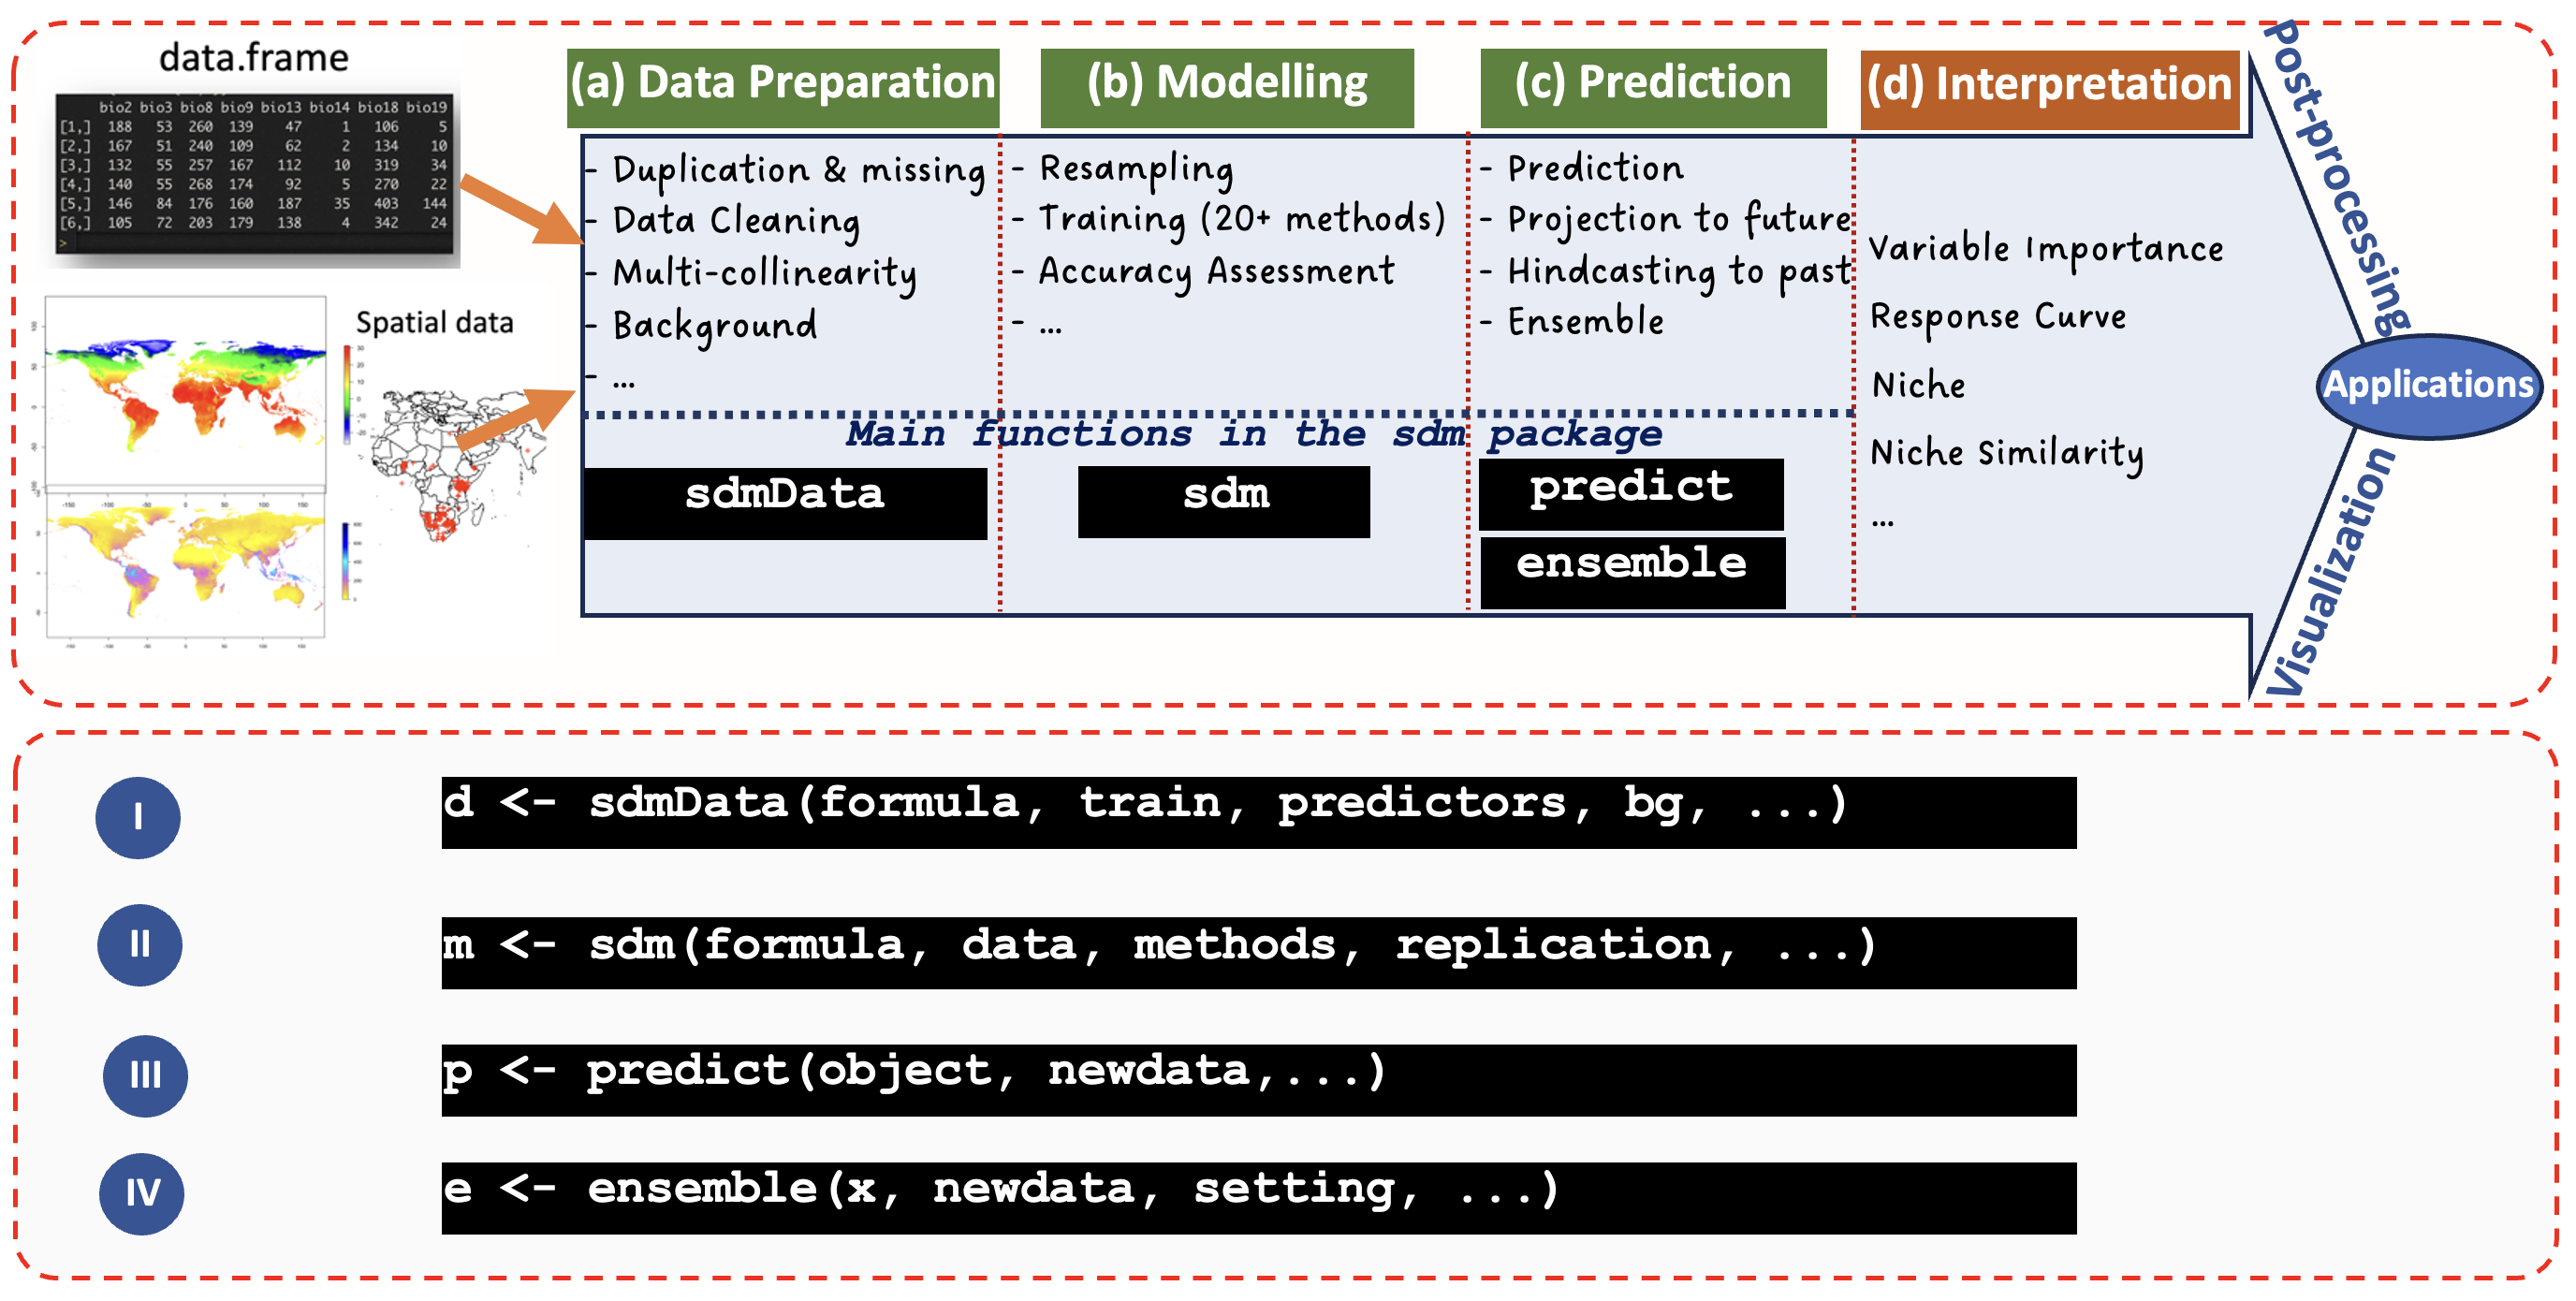
\includegraphics[width=0.9\textwidth]{Fig1.png}
    \caption{A schematic representation of the species distribution modeling workflow with the main functions, followed by their basic usages, in the \textit{'sdm'} R package.}
    \label{fig:Fig1}
\end{figure}

\subsection{\texorpdfstring{Case study: Species Distribution Modelling
of
\textit{Snow leopard}}{Case study: Species Distribution Modelling of }}\label{case-study-species-distribution-modelling-of}

To demonstrate the SDM workflow, this section is dedicated to assess and
explore
\textbf{impacts of climate change on geographical distribution of Snow leopard}
(scientific name: \textit{Panthera uncia}). We use the sdm R package,
along with some other packages, to conduct the study, and here, a step
by step guideline is provided to discuss the practical solution for
implementing the workflow and generating results in the forms of maps,
tables, and graphs.

\begin{figure}[H]
    \centering
    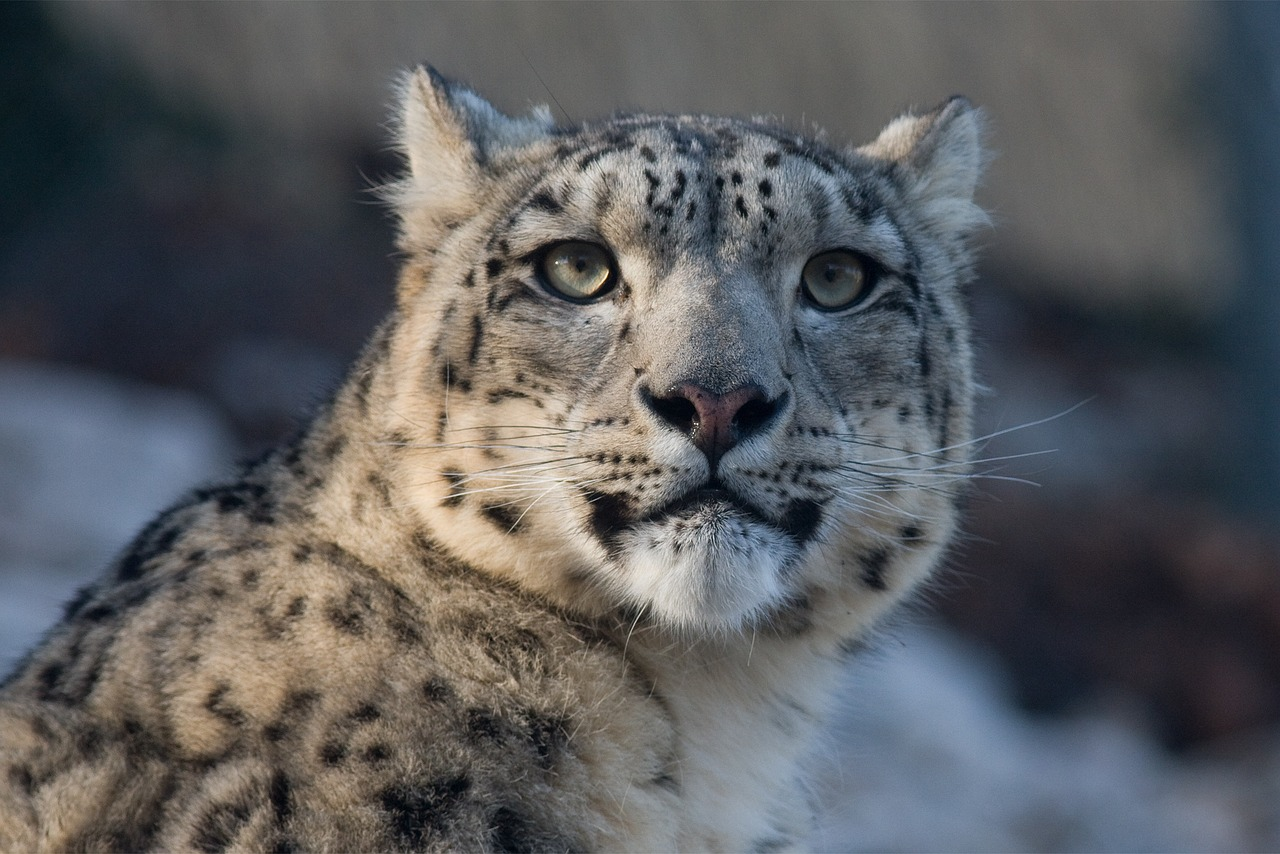
\includegraphics[width=0.3\textwidth]{snow-leopard-picture.jpg}
    \caption{Snow leopard (Panthera uncia).}
    \label{fig:Fig1}
\end{figure}

The solution to conduct the study has been provided following the main
steps in the workflow defined in Figure \ref{fig:Fig1}. The solution is
provided through the following sections:

\begin{enumerate}
\def\labelenumi{(\roman{enumi})}
\item
  \uline{Downloading data}: Here, we use R and the geodata package to
  download species data from GBIF, and climate data (for both the
  current and future times) from Worldclim.
\item
  \uline{Preparing data}: Data are checked for some issues, and get
  ready as spatial datasets for conducting SDMs.
\item
  \uline{Developing models using the sdm R package}: The main workflow
  in the sdm package (Babak Naimi and Araújo 2016) to develop and
  evaluate SDMs are demonstrated.
\item
  \uline{Predict/Project the map of habitat suitability in current and future times}:
  We predict the current distribution of the species (habitat
  suitability), and project its distribution into a future climatic
  scenario (for the year 2100).
\item
  \uline{Assess range shift in response to climate change}: Given the
  habitat suitability maps in both the current and future times, we can
  assess the magnitude and distribution of changes, and quantitatively
  measure range shifts due to climate change.
\end{enumerate}

\subsubsection{(i) Downloading Species and Climate
Data}\label{i-downloading-species-and-climate-data}

In this section, we will use R to download occurrence data for the Snow
Leopard (\textit{Panthera uncia}) from the Global Biodiversity
Information Facility (GBIF) and climate data from the WorldClim
database. These datasets will serve as the foundation for developing
species distribution models and assessing the potential impacts of
climate change on the Snow Leopard's habitat.

\uline{\textit{Species Occurrence Data}}: We will use the sp\_occurrence
function in the geodata package to download Snow Leopard occurrences
from GBIF. Occurrences are the locations where the species has been
observed (mostly cover presence-only records), providing spatial points
essential for building SDMs. Some descriptions are provided as comments
within the code:

\begin{Shaded}
\begin{Highlighting}[]
\FunctionTok{library}\NormalTok{(geodata)}
\end{Highlighting}
\end{Shaded}

\begin{verbatim}
## Loading required package: terra
\end{verbatim}

\begin{verbatim}
## terra 1.7.78
\end{verbatim}

\begin{Shaded}
\begin{Highlighting}[]
\CommentTok{\# let\textquotesingle{}s first check whether any records available on GBIF without downloading:}

\FunctionTok{sp\_occurrence}\NormalTok{(}\StringTok{"Panthera"}\NormalTok{,}\StringTok{"uncia"}\NormalTok{, }\AttributeTok{download =}\NormalTok{ F)}
\end{Highlighting}
\end{Shaded}

\begin{verbatim}
## Loading required namespace: jsonlite
\end{verbatim}

\begin{verbatim}
## [1] 197
\end{verbatim}

\begin{Shaded}
\begin{Highlighting}[]
\CommentTok{\# we have 196 records available, let\textquotesingle{}s download them as a data.frame:}

\NormalTok{sp }\OtherTok{\textless{}{-}}  \FunctionTok{sp\_occurrence}\NormalTok{(}\StringTok{"Panthera"}\NormalTok{,}\StringTok{"uncia"}\NormalTok{)}
\end{Highlighting}
\end{Shaded}

\begin{verbatim}
## 197 records found
\end{verbatim}

\begin{verbatim}
## 0-197
## 197 records downloaded
\end{verbatim}

\begin{Shaded}
\begin{Highlighting}[]
\CommentTok{\#{-}{-}{-}{-}{-}{-}{-}}
\CommentTok{\# the sp data.frame has over 100 columns, corresponding to different information}
\CommentTok{\# Some of the columns can be used to filter and exclude some records.}
\CommentTok{\# For example, the column "basisOfRecord" is a Darwin Core term that refers to }
\CommentTok{\# the specific nature of the record and can refer to one of 6 classes}

\CommentTok{\# Let\textquotesingle{}s check our records to see their frequency for different classes:}

\FunctionTok{table}\NormalTok{(sp}\SpecialCharTok{$}\NormalTok{basisOfRecord)}
\end{Highlighting}
\end{Shaded}

\begin{verbatim}
## 
##  HUMAN_OBSERVATION  MATERIAL_CITATION    MATERIAL_SAMPLE PRESERVED_SPECIMEN 
##                116                  8                  4                 69
\end{verbatim}

\begin{Shaded}
\begin{Highlighting}[]
\CommentTok{\# You may find the definition from the GBIF website:}
\CommentTok{\# https://docs.gbif.org/course{-}data{-}use/en/basis{-}of{-}record.html}

\CommentTok{\#{-}{-}{-}{-}{-}{-}}
\CommentTok{\# You can also check the years of records in our dataset:}

\FunctionTok{table}\NormalTok{(sp}\SpecialCharTok{$}\NormalTok{year)}
\end{Highlighting}
\end{Shaded}

\begin{verbatim}
## 
## 1899 1979 1998 2000 2004 2007 2008 2009 2010 2011 2012 2013 2014 2015 2016 2017 
##    1    1    1    1    2    2    2    1    1    9    6   17    9   14   15   18 
## 2018 2019 2020 2021 2022 2023 2024 
##   16   25    6    5    6   24   11
\end{verbatim}

\begin{Shaded}
\begin{Highlighting}[]
\CommentTok{\# let\textquotesingle{}s also check occurrenceStatuse column:}

\FunctionTok{table}\NormalTok{(sp}\SpecialCharTok{$}\NormalTok{occurrenceStatus) }\CommentTok{\# we are sure now all records are presence!}
\end{Highlighting}
\end{Shaded}

\begin{verbatim}
## 
## PRESENT 
##     197
\end{verbatim}

\begin{Shaded}
\begin{Highlighting}[]
\CommentTok{\# if it was not all "PRESENT", we could keep only "PRESENT" to use data as }
\CommentTok{\# a presence{-}only dataset}
\CommentTok{\#{-}{-}{-}{-}{-}{-}{-}{-}{-}{-}{-}{-}{-}{-}{-}{-}{-}{-}{-}{-}{-}{-}{-}{-}{-}{-}{-}}
\DocumentationTok{\#\#\#\#\#\# Filtering some records:}

\CommentTok{\# Given the information avaialble in "basisOfRecords" and "year" columns, we}
\CommentTok{\# want to filter data and keep appropriate records. We may use other columns}
\CommentTok{\# like coordinateUncertaintyInMeters; or we may use some specific packages }
\CommentTok{\# designed to clean GBIF data (e.g., CoordinateCleaner). But here, we do our }
\CommentTok{\# filtering based on the "basisOfRecords" and "year" columns.}

\CommentTok{\# Based on the information we checked above, we keep records with }
\CommentTok{\# basisOfRecord == "HUMAN\_OBSERVATIO" \& year \textgreater{} 1970, we use the which function:}

\NormalTok{w }\OtherTok{\textless{}{-}} \FunctionTok{which}\NormalTok{(sp}\SpecialCharTok{$}\NormalTok{basisOfRecord }\SpecialCharTok{==} \StringTok{"HUMAN\_OBSERVATION"} \SpecialCharTok{\&}\NormalTok{ sp}\SpecialCharTok{$}\NormalTok{year }\SpecialCharTok{\textgreater{}} \DecValTok{1970}\NormalTok{)}

\CommentTok{\# w keeps the record number (row number in sp data.frame) that we need to keep}

\NormalTok{sp }\OtherTok{\textless{}{-}}\NormalTok{ sp[w,] }\CommentTok{\# only keep records specified in w}

\CommentTok{\#{-}{-}{-}{-}{-}{-}}
\DocumentationTok{\#\# Get rid of all columns except coordinate columns (lon \& lat)}
\CommentTok{\# from all columns, we only keep 2 columns (lon, lat)}

\NormalTok{sp }\OtherTok{\textless{}{-}}\NormalTok{ sp[,}\FunctionTok{c}\NormalTok{(}\StringTok{\textquotesingle{}lon\textquotesingle{}}\NormalTok{,}\StringTok{\textquotesingle{}lat\textquotesingle{}}\NormalTok{)]}

\CommentTok{\# we add another column (its name can simply be "species") to which we assign }
\CommentTok{\# 1 to all records in the column as they are presence{-}only:}

\NormalTok{sp}\SpecialCharTok{$}\NormalTok{species }\OtherTok{\textless{}{-}} \DecValTok{1}

\CommentTok{\# let\textquotesingle{}s check the head of the table (data.frame) to make sure it is fine:}

\FunctionTok{head}\NormalTok{(sp)}
\end{Highlighting}
\end{Shaded}

\begin{verbatim}
##        lon      lat species
## 1 74.60183 42.50146       1
## 2 98.36646 35.58493       1
## 3 77.90942 32.34409       1
## 4 98.46910 35.55448       1
## 5 77.62451 33.91132       1
## 6 76.86968 34.31075       1
\end{verbatim}

\begin{Shaded}
\begin{Highlighting}[]
\CommentTok{\# now, we convert the sp data.frame to Spatial Points using the vect function in}
\CommentTok{\# the terra package (generates SpatVector object):}

\NormalTok{sp }\OtherTok{\textless{}{-}} \FunctionTok{vect}\NormalTok{(sp, }\FunctionTok{c}\NormalTok{(}\StringTok{\textquotesingle{}lon\textquotesingle{}}\NormalTok{,}\StringTok{\textquotesingle{}lat\textquotesingle{}}\NormalTok{))}

\NormalTok{sp }\CommentTok{\# sp, now, is a SpatVector object contining spatial points of species records}
\end{Highlighting}
\end{Shaded}

\begin{verbatim}
##  class       : SpatVector 
##  geometry    : points 
##  dimensions  : 116, 1  (geometries, attributes)
##  extent      : 71.76065, 105.8244, 27.41172, 49.8562  (xmin, xmax, ymin, ymax)
##  coord. ref. :  
##  names       : species
##  type        :   <num>
##  values      :       1
##                      1
##                      1
\end{verbatim}

\begin{Shaded}
\begin{Highlighting}[]
\CommentTok{\# let\textquotesingle{}s generate a map to see the locations of the species records:}

\CommentTok{\# We had the world map but if you don\textquotesingle{}t, you can find it on Internet!}
\NormalTok{wld }\OtherTok{\textless{}{-}} \FunctionTok{vect}\NormalTok{(}\StringTok{\textquotesingle{}world.shp\textquotesingle{}}\NormalTok{) }


\FunctionTok{plot}\NormalTok{(wld)}

\FunctionTok{points}\NormalTok{(sp,}\AttributeTok{col=}\StringTok{\textquotesingle{}red\textquotesingle{}}\NormalTok{)}
\end{Highlighting}
\end{Shaded}

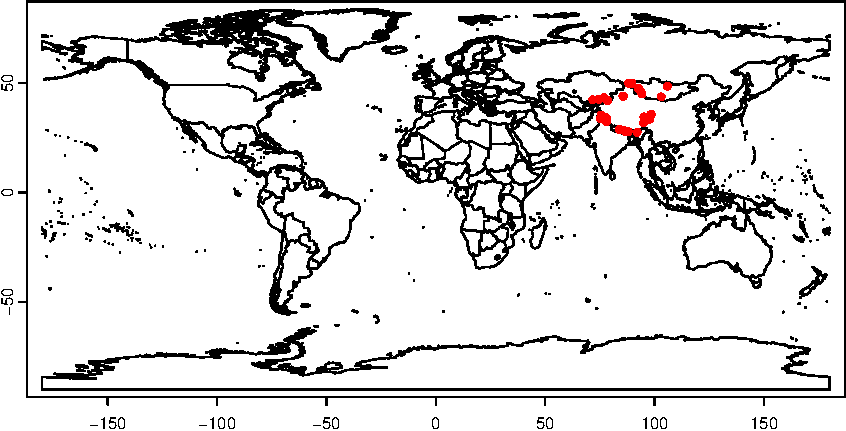
\includegraphics{sdm_R_files/figure-latex/unnamed-chunk-1-1.pdf}

\uline{\textit{Downloading Climate Data}}:

We are going to use climate data with 19 bioclimatic variables
(represent different aspects of climate condition including mean annual
temperature and precipitation, their seasonality and extreme conditions)
available in the WorldClim dataset. The bioclim variables are extracted
from monthly weather data (monthly minimum and maximum temperature and
mean precipitation). The variables are described here:
\url{https://www.worldclim.org/data/bioclim.html}

Given that the purpose of the instructions provided here is to
demonstrate how the SDM workflow can be implemented, we will use a
coarse resolution (10 minutes; approximately 20 km) dataset to make the
computation fast. However, in practice, the resolution should be
selected based on the scale of the study to ensure accurate results. The
WorldClim dataset is available on the \emph{worldclim.org} website.

We can download the dataset for both current and future time periods.
The future climate conditions are estimated using General Circulation
Models (GCMs), which simulate the Earth's climate based on various
physical processes and interactions within the atmosphere, ocean, and
land surface. These models consider different scenarios known as Shared
Socio-economic Pathways (SSPs), which reflect various potential future
conditions based on socio-economic trends and policies. SSPs provide a
comprehensive framework to analyse the impacts of different
socio-economic developments on climate change and to explore mitigation
and adaptation strategies.

The climate data for the current time (baseline), represent mean climate
condition generated from weather data recorded between 1980-2000. To
download the climate data for future times, we need to select the
appropriate GCMs (we may select several or even all GCMs for a real
study) and SSP scenarios that align with the objectives of our study.
For example, we might choose SSP2-4.5, which represents a moderate
scenario where socio-economic trends lead to stabilization in global
emissions by mid-century. Alternatively, we could select SSP5-8.5, which
represents a high-emission scenario. Under SSP5-8.5, greenhouse gas
emissions continue to rise throughout the century, leading to
significant increases in temperature and more extreme climate conditions
(also called business as usual or worst-case scenario). This scenario is
useful for understanding the potential impacts of unmitigated climate
change and helps in planning for worst-case outcomes.

For this exercise, let's download climate data for both the current time
(baseline) and future time (year 2100; it is generated based on 20 years
of data between 2081-2100) for one of GCMs and SSP5-8.5. We can use the
\emph{worldclim\_global} function to download climate data for the
current time, and cmip6\_world to download for the future. Check the
help page of the functions for more details about the usage of these
functions:

\begin{Shaded}
\begin{Highlighting}[]
\CommentTok{\# the following function, download bioclim layers with the resolution of 10 min.}

\DocumentationTok{\#\#\#\#\#\#\#\#\#\#\#\#\#\#\#\#\#\#\#\#\#\#\#\#\#\#\#\#\#\#\#\#\#\#\#\#\#\#\#\#\#\#\#\#\#\#\#\#\#\#\#\#\#\#\#\#}
\DocumentationTok{\#\#{-}{-}{-}{-}{-}\textgreater{} Downloadin climate for the Baseline (current time):}
\DocumentationTok{\#\#\#\#\#\#\#\#\#\#\#\#\#\#\#\#\#\#\#\#\#\#\#\#\#\#\#\#\#\#\#\#\#\#\#\#\#\#\#\#\#\#\#\#\#\#\#\#\#\#\#\#\#\#\#\#}

\NormalTok{bio }\OtherTok{\textless{}{-}} \FunctionTok{worldclim\_global}\NormalTok{(}\AttributeTok{var=}\StringTok{"bio"}\NormalTok{,}\AttributeTok{res=}\DecValTok{10}\NormalTok{, }\AttributeTok{path =} \FunctionTok{getwd}\NormalTok{())}

\NormalTok{bio}
\end{Highlighting}
\end{Shaded}

\begin{verbatim}
## class       : SpatRaster 
## dimensions  : 1080, 2160, 19  (nrow, ncol, nlyr)
## resolution  : 0.1666667, 0.1666667  (x, y)
## extent      : -180, 180, -90, 90  (xmin, xmax, ymin, ymax)
## coord. ref. : lon/lat WGS 84 (EPSG:4326) 
## sources     : wc2.1_10m_bio_1.tif  
##               wc2.1_10m_bio_2.tif  
##               wc2.1_10m_bio_3.tif  
##               ... and 16 more source(s)
## names       : wc2.1~bio_1, wc2.1~bio_2, wc2.1~bio_3, wc2.1~bio_4, wc2.1~bio_5, wc2.1~bio_6, ... 
## min values  :   -54.72435,     1.00000,    9.131122,       0.000,   -29.68600,   -72.50025, ... 
## max values  :    30.98764,    21.14754,  100.000000,    2363.846,    48.08275,    26.30000, ...
\end{verbatim}

\begin{Shaded}
\begin{Highlighting}[]
\CommentTok{\# let\textquotesingle{}s check the names of layers in the bio object}
\FunctionTok{names}\NormalTok{(bio)}
\end{Highlighting}
\end{Shaded}

\begin{verbatim}
##  [1] "wc2.1_10m_bio_1"  "wc2.1_10m_bio_2"  "wc2.1_10m_bio_3"  "wc2.1_10m_bio_4" 
##  [5] "wc2.1_10m_bio_5"  "wc2.1_10m_bio_6"  "wc2.1_10m_bio_7"  "wc2.1_10m_bio_8" 
##  [9] "wc2.1_10m_bio_9"  "wc2.1_10m_bio_10" "wc2.1_10m_bio_11" "wc2.1_10m_bio_12"
## [13] "wc2.1_10m_bio_13" "wc2.1_10m_bio_14" "wc2.1_10m_bio_15" "wc2.1_10m_bio_16"
## [17] "wc2.1_10m_bio_17" "wc2.1_10m_bio_18" "wc2.1_10m_bio_19"
\end{verbatim}

\begin{Shaded}
\begin{Highlighting}[]
\CommentTok{\# As you can see, the bio object contains 19 bioclim variables representing }
\CommentTok{\# climate conditions for the current time. The names are long, have information}
\CommentTok{\# about the version of the WorldClim dataset (WC\_2.1) and resolution.}

\CommentTok{\# Let\textquotesingle{}s make the names simpler (i.e., bio1, bio2, ..., bio19)}

\CommentTok{\# We can simply assign the new names:}

\FunctionTok{names}\NormalTok{(bio) }\OtherTok{\textless{}{-}} \FunctionTok{paste0}\NormalTok{(}\StringTok{\textquotesingle{}bio\textquotesingle{}}\NormalTok{,}\DecValTok{1}\SpecialCharTok{:}\DecValTok{19}\NormalTok{) }\CommentTok{\# Do you know why we used the paste0 function?}

\CommentTok{\# now, let\textquotesingle{}s check again the names of our data object:}
\FunctionTok{names}\NormalTok{(bio)}
\end{Highlighting}
\end{Shaded}

\begin{verbatim}
##  [1] "bio1"  "bio2"  "bio3"  "bio4"  "bio5"  "bio6"  "bio7"  "bio8"  "bio9" 
## [10] "bio10" "bio11" "bio12" "bio13" "bio14" "bio15" "bio16" "bio17" "bio18"
## [19] "bio19"
\end{verbatim}

\begin{Shaded}
\begin{Highlighting}[]
\CommentTok{\# Let\textquotesingle{}s visualise the first layer (Mean Annual Temperature):}


\FunctionTok{plot}\NormalTok{(bio[[}\DecValTok{1}\NormalTok{]],}\AttributeTok{main=}\StringTok{\textquotesingle{}Bio1: Mean Annual Temperature (Current time)\textquotesingle{}}\NormalTok{)}
\end{Highlighting}
\end{Shaded}

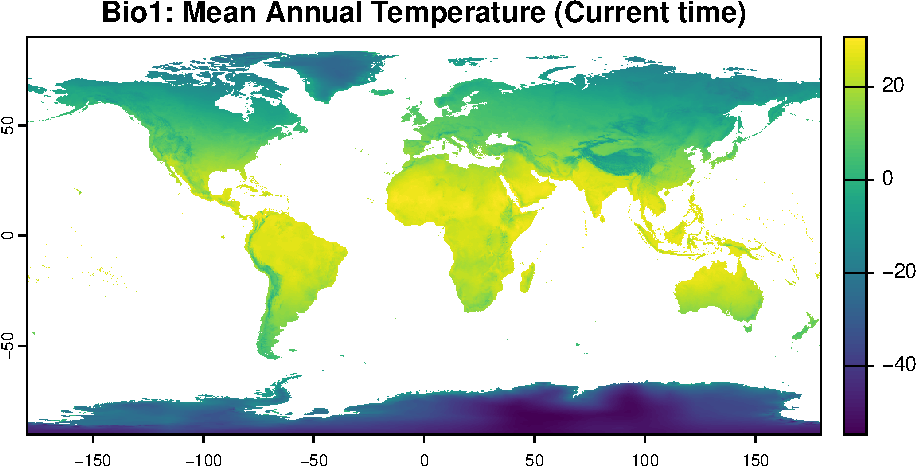
\includegraphics{sdm_R_files/figure-latex/unnamed-chunk-2-1.pdf}

\begin{Shaded}
\begin{Highlighting}[]
\CommentTok{\# and 12th layer (Mean Annual Precipitation)}

\CommentTok{\# for this one, let\textquotesingle{}s define an appropriate color palette:}

\NormalTok{cl }\OtherTok{\textless{}{-}} \FunctionTok{colorRampPalette}\NormalTok{(}\FunctionTok{c}\NormalTok{(}\StringTok{\textquotesingle{}gray\textquotesingle{}}\NormalTok{,}\StringTok{\textquotesingle{}yellow\textquotesingle{}}\NormalTok{,}\StringTok{\textquotesingle{}green\textquotesingle{}}\NormalTok{,}\StringTok{\textquotesingle{}blue\textquotesingle{}}\NormalTok{,}\StringTok{\textquotesingle{}darkblue\textquotesingle{}}\NormalTok{))}


\FunctionTok{plot}\NormalTok{(bio[[}\DecValTok{12}\NormalTok{]],}\AttributeTok{col=}\FunctionTok{cl}\NormalTok{(}\DecValTok{200}\NormalTok{),}\AttributeTok{main=}\StringTok{\textquotesingle{}Bio12:Mean Annual Precipitation (Current time)\textquotesingle{}}\NormalTok{)}
\end{Highlighting}
\end{Shaded}

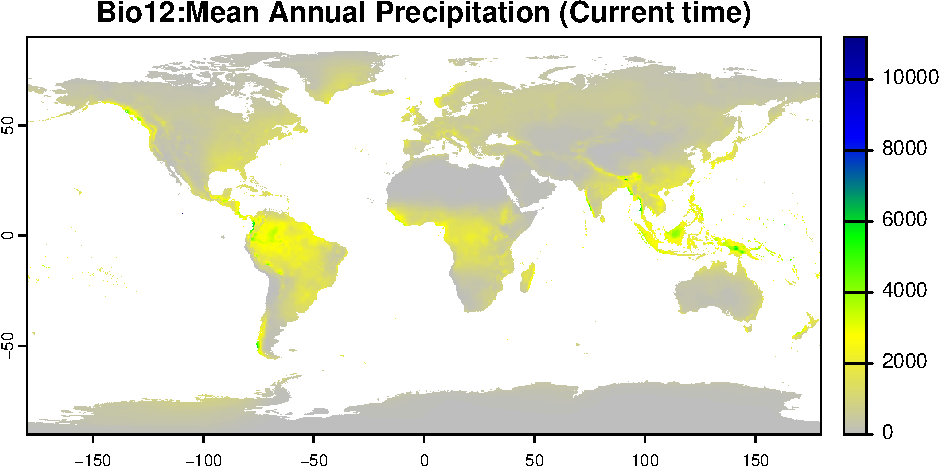
\includegraphics{sdm_R_files/figure-latex/unnamed-chunk-2-2.pdf}

\begin{Shaded}
\begin{Highlighting}[]
\DocumentationTok{\#\#\#\#\#\#\#\#\#\#\#\#\#\#\#\#\#\#\#\#\#\#\#\#\#\#\#\#\#\#\#\#\#\#\#\#\#\#\#\#\#\#\#\#\#\#\#\#\#\#\#\#\#\#\#\#}
\CommentTok{\#{-}{-}{-}{-}\textgreater{} Downloading bioclim variables for the Future time:}
\DocumentationTok{\#\#\#\#\#\#\#\#\#\#\#\#\#\#\#\#\#\#\#\#\#\#\#\#\#\#\#\#\#\#\#\#\#\#\#\#\#\#\#\#\#\#\#\#\#\#\#\#\#\#\#\#\#\#\#\#}

\CommentTok{\# To download bioclim for a future time, we need the following information:}

\DocumentationTok{\#\# GCM: Which Climate Model? (20+ GCMs are available!, here we chose: "MIROC6")}

\DocumentationTok{\#\# SSP: Which Climate Scenario? (4 different scenarios are available!)}
\CommentTok{\#{-}{-}{-}{-}{-}{-}{-}\textgreater{} ssp: 126, 245, 370, 585 (from "optimistic"....to.... "pessimistic")}

\DocumentationTok{\#\# Year: Which future time (e.g., "2081{-}2100")}

\CommentTok{\# we can also specify variables (here, we need bioclim; "bioc"), }

\DocumentationTok{\#\# res: resolution (10 arc min \textasciitilde{} equivalent to almost 20 km)}
\CommentTok{\#{-}{-}{-}{-}{-}{-}{-}{-}{-}{-}{-}}
\CommentTok{\# we can use cmip6\_world function in the geodata package to download climate }
\CommentTok{\# variables for the future times:}

\NormalTok{biof }\OtherTok{\textless{}{-}} \FunctionTok{cmip6\_world}\NormalTok{(}\AttributeTok{model=}\StringTok{"MIROC6"}\NormalTok{, }\AttributeTok{ssp=}\StringTok{\textquotesingle{}585\textquotesingle{}}\NormalTok{,}
                    \AttributeTok{time =} \StringTok{"2081{-}2100"}\NormalTok{, }\AttributeTok{var =} \StringTok{\textquotesingle{}bioc\textquotesingle{}}\NormalTok{, }\AttributeTok{res=}\DecValTok{10}\NormalTok{, }\AttributeTok{path=}\FunctionTok{getwd}\NormalTok{())}

\NormalTok{biof }
\end{Highlighting}
\end{Shaded}

\begin{verbatim}
## class       : SpatRaster 
## dimensions  : 1080, 2160, 19  (nrow, ncol, nlyr)
## resolution  : 0.1666667, 0.1666667  (x, y)
## extent      : -180, 180, -90, 90  (xmin, xmax, ymin, ymax)
## coord. ref. : lon/lat WGS 84 (EPSG:4326) 
## source      : wc2.1_10m_bioc_MIROC6_ssp585_2081-2100.tif 
## names       : bio01, bio02, bio03,  bio04, bio05, bio06, ... 
## min values  : -50.3,  -1.9, -10.6,   13.4,   -26, -68.4, ... 
## max values  :  36.3,  22.5,  95.4, 2250.5,    55,  27.8, ...
\end{verbatim}

\begin{Shaded}
\begin{Highlighting}[]
\CommentTok{\# let\textquotesingle{}s check the names of the biof object which contains bioclim variables of}
\CommentTok{\# future (year: 2100) for the worst{-}case scenario (ssp585):}

\FunctionTok{names}\NormalTok{(biof) }
\end{Highlighting}
\end{Shaded}

\begin{verbatim}
##  [1] "bio01" "bio02" "bio03" "bio04" "bio05" "bio06" "bio07" "bio08" "bio09"
## [10] "bio10" "bio11" "bio12" "bio13" "bio14" "bio15" "bio16" "bio17" "bio18"
## [19] "bio19"
\end{verbatim}

\begin{Shaded}
\begin{Highlighting}[]
\CommentTok{\# For our modelling practice, the names of bioclim layers in the current and }
\CommentTok{\# future time should be exactly the same, so since the order of the layers in }
\CommentTok{\# bio and biof is the same, we can simply assign the names of biof to be the }
\CommentTok{\# same as bio:}

\FunctionTok{names}\NormalTok{(biof) }\OtherTok{\textless{}{-}} \FunctionTok{names}\NormalTok{(bio)}


\CommentTok{\# let\textquotesingle{}s visualise precipitation for the future time:}

\FunctionTok{plot}\NormalTok{(biof[[}\DecValTok{12}\NormalTok{]],}\AttributeTok{col=}\FunctionTok{cl}\NormalTok{(}\DecValTok{200}\NormalTok{), }
     \AttributeTok{main=}\StringTok{"Bio12: Mean Annual Precipitation (Year:2100; SSP{-}585)"}\NormalTok{)}
\end{Highlighting}
\end{Shaded}

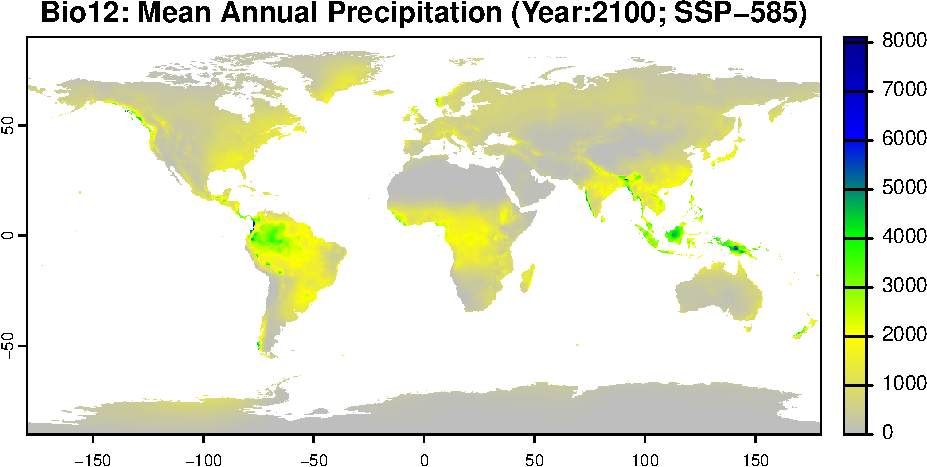
\includegraphics{sdm_R_files/figure-latex/unnamed-chunk-2-3.pdf}

\subsubsection{(ii) Data preparation}\label{ii-data-preparation}

After downloading data, we need to take some steps to prepare data for
modelling.

While statistical methods can be employed to identify outliers of the
species data, a visual inspection of the map with species locations
suggests that the points in North America may be outliers. This
suspicion can be further validated by comparing these points with the
species' range map provided by the IUCN. Therefore, we can exclude the
outlier records. However, if the study area to train the model is
selected and the outliers are located outside of the study area, the
outliers will not be considered in the modelling procedure (i.e., no
need to exclude them).

\uline{\textit{Selecting study area}}:

Although the purpose of our case study is to generate \textbf{global}
potential distribution of species, we may select a realistic study area
which can be an area potentially accessible to the species. Since the
background records are generated within the study area, it is important
to select a reasonable area to train SDMs. We may use a biogeographical
map to overlap presence records and select the polygons intersected
which species presence locations and conider them as the study area.
Alternatively, we can approximately specify the area by choosing its
upper left and lower right which give us the minimum and maximum x and y
coordinates to make an extent object using the terra package.

\begin{Shaded}
\begin{Highlighting}[]
\FunctionTok{library}\NormalTok{(terra)}

\FunctionTok{plot}\NormalTok{(wld)}

\NormalTok{bnd }\OtherTok{\textless{}{-}} \FunctionTok{ext}\NormalTok{(}\FunctionTok{c}\NormalTok{(}\DecValTok{60}\NormalTok{,}\DecValTok{120}\NormalTok{,}\DecValTok{10}\NormalTok{,}\DecValTok{60}\NormalTok{)) }\CommentTok{\# spatial extent with c(X\_min, X\_max, Y\_min, Y\_max)}

\FunctionTok{points}\NormalTok{(sp,}\AttributeTok{col=}\StringTok{\textquotesingle{}red\textquotesingle{}}\NormalTok{)}

\FunctionTok{plot}\NormalTok{(bnd,}\AttributeTok{add=}\NormalTok{T,}\AttributeTok{border=}\StringTok{\textquotesingle{}blue\textquotesingle{}}\NormalTok{)}
\end{Highlighting}
\end{Shaded}

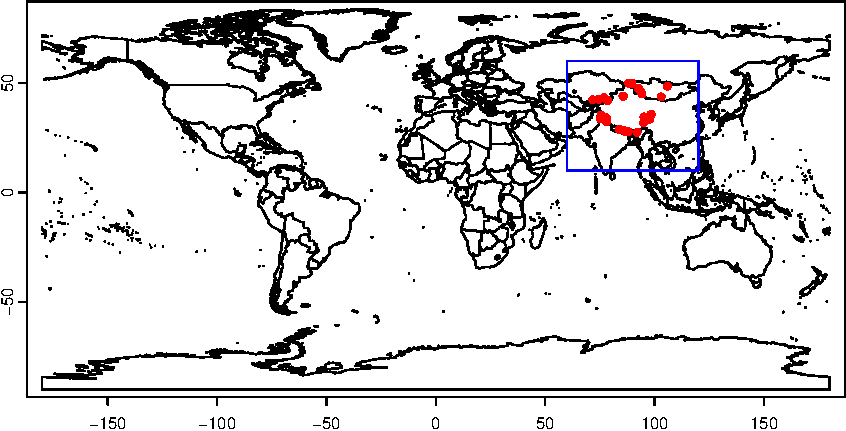
\includegraphics{sdm_R_files/figure-latex/unnamed-chunk-3-1.pdf}

\uline{\textit{Cropping Climate Data to the extent defined as the study area}}:

As mentioned earlier, when the species records are presence-only, we
need to consider a realistic area (areas potentially accessible for the
species) to calibrate (train) SDMs where the background records are
drawn. Here, the specified extent (the rectangle) is used as the study
area to train SDMs but we will use the models to predict/project across
the world.

The following code crops the bioclim variables of the current time
within the specified extent (bnd object). We don't crop the future
dataset (biof) as the model training uses on the variables in the
current time:

\begin{Shaded}
\begin{Highlighting}[]
\CommentTok{\# the extent specified earlier:}
\NormalTok{bnd}
\end{Highlighting}
\end{Shaded}

\begin{verbatim}
## SpatExtent : 60, 120, 10, 60 (xmin, xmax, ymin, ymax)
\end{verbatim}

\begin{Shaded}
\begin{Highlighting}[]
\NormalTok{bioc }\OtherTok{\textless{}{-}} \FunctionTok{crop}\NormalTok{(bio, bnd) }\CommentTok{\# crop bio object within the bnd extent}

\CommentTok{\# let\textquotesingle{}s visualise a layer from "bioc" and add the species occurrences to the map:}

\FunctionTok{plot}\NormalTok{(bioc[[}\DecValTok{1}\NormalTok{]],}\AttributeTok{main=}\StringTok{\textquotesingle{}Bio1 (cropped)\textquotesingle{}}\NormalTok{)}

\FunctionTok{points}\NormalTok{(sp,}\AttributeTok{col=}\StringTok{\textquotesingle{}red\textquotesingle{}}\NormalTok{)}
\end{Highlighting}
\end{Shaded}

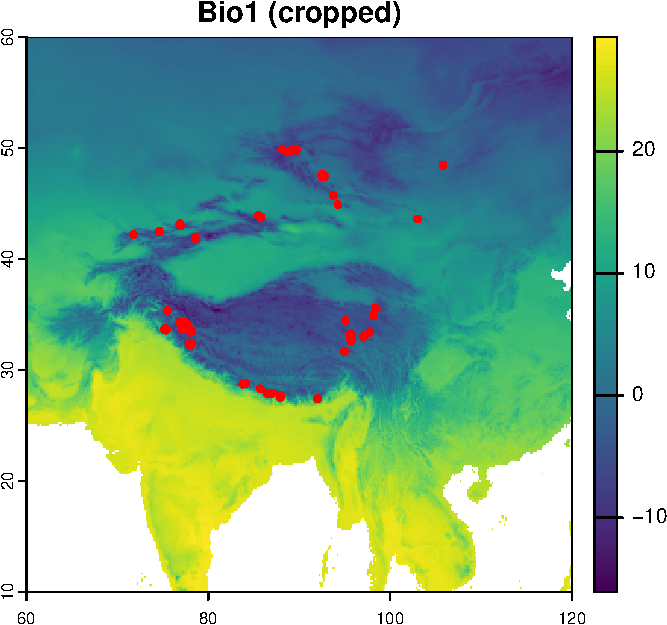
\includegraphics{sdm_R_files/figure-latex/unnamed-chunk-4-1.pdf}

\uline{\textit{Multi-collinearity}}:

When we have two or more numerical predictor variables that are strongly
correlated, the data are subjected to the issue of multi-collinearity
(also called collinearity) (Dormann et al. 2013). Some modelling
methods, such as GLMs, may be sensitive to the collinearity issue as
their parameterisation can be affected. Even if a modelling method is
not sensitive, excluding the collinear variables is a good practice
given the parsimony rule to avoid redundant information in the model
which makes it un-necessarily complex.

Several approaches are available to deal with collinearity issue. One
approach is to transform the environmental variables into a new set of
variables using Principle Component Analysis (PCA), an ordination method
for reducing data dimensions and generate new, uncorrelated variables.
This can be done using the \texttt{pca} function, or by specifying the
\texttt{pca} term in the formula in the \texttt{sdmData} function.

Another approach is to identify and exclude variables that show signs of
collinearity. To identify collinear variables, a simple pairwise
correlation test can be conducted between each pair of variables (a
correlation greater than 0.7 is indicative of collinearity).
Alternatively, the variance inflation factor (VIF) can be measured for
each variable, representing how much of a variable's variance can be
explained by other variables (a VIF greater than 10 is a sign of
collinearity).

A popular hybrid approach was introduced by Naimi et al.~(2014) to
measure VIF or combination of VIF and correlation coefficient through a
stepwise procedure (Babak Naimi et al. 2014). Two functions implemented
in the usdm package can be used here including \texttt{vifstep}, and
\texttt{vifcor}. To deal with collinearity, one of these two methods
should be used. \texttt{vifstep} checks the VIF metric for all numerical
predictor variables and identifies the variable with the maximum VIF for
exclusion if it exceeds the specified threshold (default=10). This
procedure is repeated step by step until all the remained variables have
VIF values below the threshold.

Alternatively, \texttt{vifcor} checks the correlation coefficient for
all possible pairs of variables, and identifies the pair with the
maximum correlation. If it exceeds the specified threshold (e.g., 0.7),
one of the two variables in the pair is excluded. To make decision that
which one should be excluded, VIF is calculated for both variables in
the pair and the one with the greater VIF is excluded. The procedure is
repeated step by step until none of the remaining pairs have a
correlation greater than the threshold (Babak Naimi et al. 2014).

Here, we test the collinearity issue among the 19 bioclim variables in
the current time using the \texttt{vifstep} function, and exclude
collinear variables from all datasets (current and future times):

\begin{Shaded}
\begin{Highlighting}[]
\FunctionTok{library}\NormalTok{(usdm) }\CommentTok{\# contains the functions to deal with collinearity}

\NormalTok{v }\OtherTok{\textless{}{-}} \FunctionTok{vifstep}\NormalTok{(bioc, }\AttributeTok{th=}\DecValTok{10}\NormalTok{) }\CommentTok{\# checks collinearity with vifstep and threshold of 10}

\CommentTok{\# here is the output of vifstep, reporting which variables should be excluded:}
\NormalTok{v}
\end{Highlighting}
\end{Shaded}

\begin{verbatim}
## 10 variables from the 19 input variables have collinearity problem: 
##  
## bio6 bio11 bio10 bio7 bio16 bio1 bio12 bio17 bio4 bio5 
## 
## After excluding the collinear variables, the linear correlation coefficients ranges between: 
## min correlation ( bio3 ~ bio2 ):  -0.005749341 
## max correlation ( bio18 ~ bio13 ):  0.721448 
## 
## ---------- VIFs of the remained variables -------- 
##   Variables      VIF
## 1      bio2 2.537522
## 2      bio3 2.681313
## 3      bio8 1.431894
## 4      bio9 2.126017
## 5     bio13 4.116040
## 6     bio14 2.463484
## 7     bio15 2.264739
## 8     bio18 2.866524
## 9     bio19 1.371750
\end{verbatim}

\begin{Shaded}
\begin{Highlighting}[]
\CommentTok{\# Now, let\textquotesingle{}s exclude the collinear varibales from all data objects:}
\CommentTok{\# ... exclude collinear variables from bioc (cropped bio) based on "v"}
\NormalTok{bioc }\OtherTok{\textless{}{-}} \FunctionTok{exclude}\NormalTok{(bioc,v)}

\CommentTok{\# now, you can see that bioc has the selected variables:}

\NormalTok{bioc}
\end{Highlighting}
\end{Shaded}

\begin{verbatim}
## class       : SpatRaster 
## dimensions  : 300, 360, 9  (nrow, ncol, nlyr)
## resolution  : 0.1666667, 0.1666667  (x, y)
## extent      : 60, 120, 10, 60  (xmin, xmax, ymin, ymax)
## coord. ref. : lon/lat WGS 84 (EPSG:4326) 
## source(s)   : memory
## names       :     bio2,     bio3,      bio8,      bio9, bio13, bio14, ... 
## min values  :  3.83750, 14.90886, -15.74217, -32.20467,     3,     0, ... 
## max values  : 18.35242, 76.99110,  36.88192,  34.43004,  2381,    77, ...
\end{verbatim}

\begin{Shaded}
\begin{Highlighting}[]
\CommentTok{\# let\textquotesingle{}s do it for objects the objects of global scale (bio, biof):}
\NormalTok{bio }\OtherTok{\textless{}{-}} \FunctionTok{exclude}\NormalTok{(bio, v)}

\NormalTok{biof }\OtherTok{\textless{}{-}} \FunctionTok{exclude}\NormalTok{(biof, v)}

\CommentTok{\# If you want to save the new data objects, you can use the writeRaster function}
\CommentTok{\# Example:....\textgreater{} bio \textless{}{-} writeRaster(bio, filename="bioclim\_selected\_current.tif")}

\CommentTok{\#{-}{-}{-}{-}{-}{-}{-}{-}{-}{-}{-}}
\CommentTok{\# as you can see, the selected variables are in bio (and in biof and bioc):}

\NormalTok{bio}
\end{Highlighting}
\end{Shaded}

\begin{verbatim}
## class       : SpatRaster 
## dimensions  : 1080, 2160, 9  (nrow, ncol, nlyr)
## resolution  : 0.1666667, 0.1666667  (x, y)
## extent      : -180, 180, -90, 90  (xmin, xmax, ymin, ymax)
## coord. ref. : lon/lat WGS 84 (EPSG:4326) 
## sources     : wc2.1_10m_bio_2.tif  
##               wc2.1_10m_bio_3.tif  
##               wc2.1_10m_bio_8.tif  
##               ... and 6 more source(s)
## names       :     bio2,       bio3,      bio8,      bio9, bio13, bio14, ... 
## min values  :  1.00000,   9.131122, -66.29942, -54.26688,     0,     0, ... 
## max values  : 21.14754, 100.000000,  37.70479,  37.43358,  2381,   484, ...
\end{verbatim}

\subsubsection{(iii) Developing models using the sdm R
package:}\label{iii-developing-models-using-the-sdm-r-package}

Now, we have both species (response) and climate (predictors) variables
ready to implement the modelling workflow using the sdm package. The
package can be installed normally from CRAN or from Github using:
\texttt{devtools::install\_github(\textquotesingle{}babaknaimi/sdm\textquotesingle{}))}.
\textbf{To get all modelling methods available for training SDMs, some
additional packages also need to be installed. You may use the
\texttt{installAll()} function one time after installing sdm to get all
required packages installed on your machine.}

In the sdm package, two user-friendly functions should be used to
develop the models. First, an sdmdata object should be created using the
\texttt{sdmData} function, then, models are trained and evaluated using
the \texttt{sdm} function.

The usage of the function:

\texttt{sdmData(formula,train,predictors,test,bg,filename,crs,impute,metadata,...)}

The \texttt{sdmData} function requires both species and predictor
variables and several issues with data (e.g., duplications, missing
values) and inconsistencies (e.g., mis-match in coordinate reference
systems) are checked and fixed by this function. It has a
\texttt{formula} interface (check the following box) which provides
flexibility for users to control data structure and formats, and apply
several functions on data.

\begin{mdframed}[backgroundcolor=gray!10, linecolor=black!75, linewidth=2pt, roundcorner=5pt, shadow=true,frametitle={\textbf{BOX 1: \uline{Formula interface in the sdmData function}}}]

The "formula" interface in R is a powerful and versatile tool that simplifies the specification of statistical models. Central to many modeling functions in R, the formula interface allows users to define the relationship between the dependent and independent variables in a clear and concise manner. This interface uses a symbolic syntax to represent models, making it intuitive and accessible for users to specify complex models without delving into the underlying mathematical details.

At its core, the formula interface uses a simple syntax: the tilde (~) operator separates the response variable on the left from the predictor variables on the right. For example, in the formula y ~ x1 + x2, y is the dependent variable (species), and x1 and x2 are the independent variables (predictors; environmental variables). In the sdm R package, the formula interface has been extended to support specifying different types of data (e.g., categorical/factor variables, time, coordinates), and provide flexibility in controlling data processing and modelling by users. 

The formula interface is implemented as the first argument in the two main functions in the sdm package, including \texttt{sdmData}, and \texttt{sdm} Following syntax are examples to illustrate how the formula interface in the sdm package provides flexibility which contributes to make the package user-friendly.
The formula in both the  \texttt{sdmData}, and \texttt{sdm} functions is used to specify the species in the left-hand side, and predictors in the right-hand side. Let’s assume the name of species in our data is “species”, and we used three predictors named “bio1”, “bio2”, and “bio3”, then, the formula can be defined as:

\texttt{sdmData(species \textasciitilde{} bio1 + bio2 + bio3, …)}

We can simply use “.” in the right-hand side to avoid typing all the variables names, meaning use all existing variables:


\texttt{species \textasciitilde{} .}


\uline{\textit{Categorical variables}}: If we have categorical variables in our dataset, we can explicitly specify them by using the term of “factor” or simply “f” in the formula (refers to factor data type that is used in R for handling categorical data). Let’s assume our categorical variable is “landuse”, then the formula would be:


\texttt{species \textasciitilde{} . + f(landuse)}


\uline{\textit{Spatial coordinates}}: When we use spatial data objects (e.g., spatial points and raster), coordinates of species locations are extracted from the dataset, but when the input dataset is a data.frame and if spatial coordinates are available (e.g., two columns of the data.frame are coordinates with the names of “lon” and “lat”), we can specify them in the formula:

\texttt{species \textasciitilde{} . + f(landuse) + coords(lon+lat)}

\uline{\textit{Time (temporal data)}}: If data/time records are available (e.g., date of species observations), it can be specified using the term of “time”:

\texttt{species \textasciitilde{} . + f(landuse) + coords(lon+lat) + time(eventDate)}

\uline{\textit{Multiple species}}: The sdm package supports modelling for simultaneously multiple species. When we have multiple species in the dataset, their names can be included in the lef-hand side of the formula as:

\texttt{species1 + species2 + species3 \textasciitilde{} . + f(landuse)}

If the left-hand side of the formula is left empty, the package tries to detect the available species data in the input dataset by assuming all variables having binomial records (1 and 0), are species variables (presence-absence):

\texttt{\textasciitilde{} . + f(landuse)}


\uline{\textit{Selecting variables}}: Another formula term in the sdm package, “select”, can be used in data preparation procedure to select a subset of variables using a variable selection procedure. For instance, assessing the issue of multi-collinearity in data may be resulted to exclude some problematic variables and keep a subset. The multi-collinearity assessment in the sdm package uses two different approaches, “vifcor” and “vifstep” (Naimi et al., 2014), implemented in the usdm R package. By using “select”, a user can specify names of (numerical) variables for which the collinearity should be checked:
The following example checks collinearity for all numeric variables using the vifstep function given the threshold of 10:


\texttt{species \textasciitilde{} . + select(., method="vifstep",th=10) }

The following example checks collinearity for all numeric variables except “bio1” using the vifcor function given the threshold of 0.7:

\texttt{species\textasciitilde{} . + select(. – bio1, method="vifcor", th=0.7) }

\uline{\textit{Scaling the variables}}: Given that the range (gradient) of predictor variables is usually different and not directly comparable to each other, transforming them to a similar range (scaling) can significantly enhance model convergence and performance. Scaling ensures that each predictor variable contributes equally to the model, preventing variables with larger ranges from disproportionately influencing the results. This is especially important for modeling algorithms sensitive to the scale of input data, can also facilitate the optimization process, leading to faster and more stable convergence of the model parameters. 

In The sdm package, it is straightforward and easy to use the scale term in the formula to standardize predictor variables before model fitting. By using the scale function, users can ensure that their models are robust, efficient, and interpretable, as this step is a best practice in the species distribution modeling workflow, reinforcing the reliability and effectiveness of the models developed using the sdm package. Two scaling methods are available in the package, “minmax” (default) transforms the data to a range between 0 and 1, and “center” scales each variable by subtracting its mean, divided by its standard deviation:

\texttt{species \textasciitilde{} . + scale(.) \# scaling of all variables using the default method ("minmax") }

\texttt{species \textasciitilde{} . + scale(bio1 + bio2) \# scaling of only bio1 and bio2 variables}

\texttt{species \textasciitilde{} . + scale(., method="center") \# scaling all using the method of "center"}
 
\uline{\textit{Principle component analysis (PCA)}}: PCA is a valuable technique for reducing the dimensionality of data and addressing issues of multi-collinearity among predictor variables. In the context of species distribution modeling, PCA transforms the original numerical variables into a set of uncorrelated components, which can then be used as predictors in the model. This transformation helps in simplifying the model by retaining only the most significant components, thereby enhancing computational efficiency and model interpretability. The sdm R package facilitates the incorporation of PCA directly within the formula interface. By specifying a PCA term in the formula, users can automatically transform the numerical variables into principal components, selecting either the first n components or those that explain a specified portion of the total variance (e.g., 80%). The option to scale the variables before PCA further ensures that each variable contributes equally to the analysis. This integration of PCA within the sdm package streamlines the workflow, allowing for more effective data preprocessing and robust model development:

The following line of code re-scales and transforms all numeric variables using PCA and selects the first two generated components to be used as predictor variables in the SDM workflow:
 
\texttt{species \textasciitilde{} pca(. , n=2 , scale = TRUE) }

Alternatively if n = "auto", the function identifies the best number of components which is the default behaviour; i.e., the following line of code is equivalent to: species \textasciitilde{} pca(.) :

\texttt{species \textasciitilde{} pca(. , n= "auto", scale = TRUE)  }

Or you may specify the minimum percentage of variability explained by the selected components:

\texttt{species \textasciitilde{} pca(. , n=0.8 , scale = TRUE) }

By using the formula interface, users can leverage R's extensive statistical modeling capabilities with ease. This interface not only promotes consistency across different modeling functions but also enhances readability and reproducibility of the code. As such, the formula interface is an essential feature of R that empowers users to build, analyse, and interpret a wide array of statistical models efficiently.

\end{mdframed}

The sdmdata object, generated by the \texttt{sdmData} function, is like
a database containing all species and environmental records as well as
additional information (spatial coordinates, temporal dimension,
grouping factors, coordinate reference system, metadata, etc.).

Let's create the \texttt{sdmdata} object given the species data
(\texttt{SpatVector} object: \texttt{sp}) and the climate variables
(\texttt{SpatRaster} object: \texttt{bioc}). In the species data
(\texttt{sp}), we had the presence-only values (1) assigned to a column
named \texttt{species}.

\uline{\textit{Backgrounds (pseudo-absences)}}: Since the species
dataset is presence-only, we need to generate background
(pseudo-absence) records. Several methods are available to generate
backgrounds (you may check the help page of the \texttt{background}
function in the sdm package). For this purpose, we use the method of
\texttt{gRandom} which generates background randomly in the geographic
space. The setting to generate background records can be provided
through the \texttt{bg} argument to the \texttt{sdmData} function using
a list. In addition to the method, \texttt{n} (the number of background
records), and some optional arguments can be provided (e.g.,
\texttt{bias} which is a raster file can be used for a target-based
background generation).

\begin{Shaded}
\begin{Highlighting}[]
\FunctionTok{library}\NormalTok{(sdm)}
\end{Highlighting}
\end{Shaded}

\begin{verbatim}
## sdm 1.2-52 (2024-10-23)
\end{verbatim}

\begin{Shaded}
\begin{Highlighting}[]
\DocumentationTok{\#\# the first step in the sdm package is to create the data object:}
\CommentTok{\# {-}{-}{-}\textgreater{} 500 background records will be generated using "gRandom":}
\NormalTok{d }\OtherTok{\textless{}{-}} \FunctionTok{sdmData}\NormalTok{(species}\SpecialCharTok{\textasciitilde{}}\NormalTok{.,}\AttributeTok{train=}\NormalTok{sp,}\AttributeTok{predictors=}\NormalTok{bioc,}\AttributeTok{bg=}\FunctionTok{list}\NormalTok{(}\AttributeTok{n=}\DecValTok{500}\NormalTok{,}\AttributeTok{method=}\StringTok{\textquotesingle{}gRandom\textquotesingle{}}\NormalTok{))}

\CommentTok{\# you may get a summary from the created object by executing the object:}

\NormalTok{d}
\end{Highlighting}
\end{Shaded}

\begin{verbatim}
## class                                 : sdmdata 
## =========================================================== 
## number of species                     :  1 
## species names                         :  species 
## number of features                    :  9 
## feature names                         :  bio2, bio3, bio8, ... 
## type                                  :  Presence-Background 
## has independent test data?             :  FALSE 
## number of records                     :  616 
## has Coordinates?                      :  TRUE
\end{verbatim}

\uline{\textit{Modelling and Evaluation}}: After creating the data
object (\texttt{sdmdata}), the \texttt{sdm} function can be used to
train and evaluate multiple models in parallel. 20+ modelling methods
are available in the package. The models can be extended by users
through using the \texttt{add} function. The list of existing methods
can be checked using getmethodNames function:

\begin{Shaded}
\begin{Highlighting}[]
\FunctionTok{getmethodNames}\NormalTok{(}\AttributeTok{alt=}\NormalTok{F)}
\end{Highlighting}
\end{Shaded}

\begin{verbatim}
##  [1] "bioclim"       "bioclim.dismo" "brt"           "cart"         
##  [5] "domain.dismo"  "fda"           "gam"           "glm"          
##  [9] "glmnet"        "glmpoly"       "mahal.dismo"   "mars"         
## [13] "maxent"        "maxlike"       "maxNet"        "mda"          
## [17] "mlp"           "ranger"        "rbf"           "rf"           
## [21] "rpart"         "svm"
\end{verbatim}

Usage of \texttt{sdm}:

\texttt{sdm(formula,\ data,\ methods,...)}

In the sdm function, \texttt{formula} (to specify the structure of the
model), \texttt{data} (the output of \texttt{sdmData}), and
\texttt{methods} (to specify the names of modelling methods) are the
minimum inputs to get the function works. Some additional inputs can be
provided to specify settings for the \texttt{replication} methods which
split data to training and test partitions for evaluating the models.
The following sub-section provides some details about model evaluation:

\uline{\textit{Replication}}: To evaluate the models, if an independent
dataset is available, thay can be used to test the performance of
models. If that is the case, the independent test data can be provided
to the \texttt{sdmData} function. However, such independent data are not
available in most situations. Therefore, an alternative solution might
be used which is to split the data into two partitions using a
re-sampling method. Several re-sampling methods are available in the sdm
package including ``sub-sampling'' (uses a random sampling without
replacement to divide data given the percentage specified by a user; for
example, if \texttt{test.percent} = 30 is specified by a user, 30\% of
records are randomly selected to be used as test data and the rest for
training the models), ``bootstrapping'' (uses a random sampling with
replacement; for this method, a random sample with replacement and with
the same size as the original data is drawn from the records which are
used for training the models, and the records that are not selected in
the sample are used as the test data), and ``cross-validation'' (divide
data into n folds/partitions {[}\texttt{cv.fold} specified by a user{]}
at the beginning of the procedure and the models are trained n times and
every time one of the folds is selected as the test data). A user can
specify one or more of these methods through the \texttt{replication}
argument, and the procedure can be repeated multiple times if a user add
the \texttt{n} argument with the number of replications.

Here is an example of using the sdm function where we chose 5 modelling
method, also used sub-sampling with 30\% of data for test dataset, and
repeated the procedure 3 times:

\begin{Shaded}
\begin{Highlighting}[]
\DocumentationTok{\#\# second step: to train and evaluate the models:}

\CommentTok{\#{-}{-}{-}{-}\textgreater{} 5 modelling methods are used: }
\CommentTok{\# =======\textgreater{}\textgreater{} glmp: polynomial generalised linear model; }
\CommentTok{\# =======\textgreater{}\textgreater{} brt: Boosted Regression Trees; }
\CommentTok{\# =======\textgreater{}\textgreater{} rf: Random Foress; }
\CommentTok{\# =======\textgreater{}\textgreater{} maxent: Maximum Entropy; }
\CommentTok{\# =======\textgreater{}\textgreater{} svm: Support Vector Machine; }

\CommentTok{\#{-}{-}{-}{-}\textgreater{} Replication method: sub{-}sampling (with 30 \% of test data; repeats 3 times)}

\NormalTok{m }\OtherTok{\textless{}{-}} \FunctionTok{sdm}\NormalTok{(species}\SpecialCharTok{\textasciitilde{}}\NormalTok{., d, }\AttributeTok{methods =} \FunctionTok{c}\NormalTok{(}\StringTok{\textquotesingle{}glm\textquotesingle{}}\NormalTok{,}\StringTok{\textquotesingle{}brt\textquotesingle{}}\NormalTok{,}\StringTok{\textquotesingle{}rf\textquotesingle{}}\NormalTok{,}\StringTok{\textquotesingle{}maxent\textquotesingle{}}\NormalTok{,}\StringTok{\textquotesingle{}svm\textquotesingle{}}\NormalTok{),}
         \AttributeTok{replication=}\StringTok{\textquotesingle{}sub\textquotesingle{}}\NormalTok{, }\AttributeTok{test.p=}\DecValTok{30}\NormalTok{, }\AttributeTok{n =} \DecValTok{3}\NormalTok{)}


\CommentTok{\# to see a summary of the modelling outputs, you may check the object:}

\NormalTok{m}
\end{Highlighting}
\end{Shaded}

\begin{verbatim}
## class                                 : sdmModels 
## ======================================================== 
## number of species                     :  1 
## number of modelling methods           :  5 
## names of modelling methods            :  glm, brt, rf, maxent, svm 
## replicate.methods (data partitioning) :  subsampling 
## number of replicates (each method)    :  3 
## toral number of replicates per model  :  3 (per species) 
## test percentage (in subsampling)      :  30 
## ------------------------------------------
## model run success percentage (per species)  :
## ------------------------------------------
## method          species          
## ---------------------- 
## glm        :        100   %
## brt        :        100   %
## rf         :        100   %
## maxent     :        100   %
## svm        :        100   %
## 
## ###################################################################
## model Mean performance (per species), using test dataset (generated using partitioning):
## -------------------------------------------------------------------------------
## 
##  ## species   :  species 
## =========================
## 
## methods    :     AUC     |     COR     |     TSS     |     Deviance 
## -------------------------------------------------------------------------
## glm        :     0.87    |     0.58    |     0.62    |     0.65     
## brt        :     0.93    |     0.74    |     0.73    |     0.59     
## rf         :     0.96    |     0.82    |     0.83    |     0.36     
## maxent     :     0.94    |     0.74    |     0.81    |     0.47     
## svm        :     0.95    |     0.77    |     0.84    |     0.42
\end{verbatim}

As you can see above, in the summary information provided from the
\texttt{sdmModels} object, 3 models were trained for each modelling
method (15 models in total), and they were evaluated using multiple
accuracy metrics (e.g., AUC, TSS). Mean values of these metrics can
provide a quick way to compare the performance of different methods.

There is a user-friendly and interactive way to explore part of the
results available within the sdmModels object through using the
\texttt{gui} function. This function opens a graphical user interface
with different parts (windows/tabs) which allows a user to explore the
results (evaluation, variable importance, etc.). You may simply use the
following line of code to use the function:

\texttt{gui(m)}

\hfill\break
\hfill\break
\hfill\break

\begin{mdframed}[backgroundcolor=gray!10, linecolor=black!75, linewidth=2pt, roundcorner=5pt, shadow=true,frametitle={\textbf{BOX 2: \uline{Model evaluations for SDMs}}}]

Evaluating the performance of models is a crucial step in species distribution modeling (SDM) to ensure the accuracy and reliability of predictions. Several evaluation metrics are commonly used to assess how well a model predicts the occurrence of species based on known data. Here are some of the most widely used methods:


\textbf{\large Confusion Matrix and Threshold-Based Metrics}

The confusion matrix is a tool used to evaluate the performance of a models when the response variable is categorical (or classes such as presence and absence). The confusion matric tool allows to compare the observed values (presence/absences) with the predicted presence and absences. Since SDMs are usually generating probability of occurrences (or habitat suitability values) rather than presence/absence values, a threshold is needed to first convert the predicted probabilities to presence/absences, then make the confusion matrix and calculate the accuracy metrics. Therefore, the metrics generated based on a confusion matrix is also called \textbf{threshold-based} metrics. The matrix is composed of four key components:


\begin{figure}[H]
    \centering
    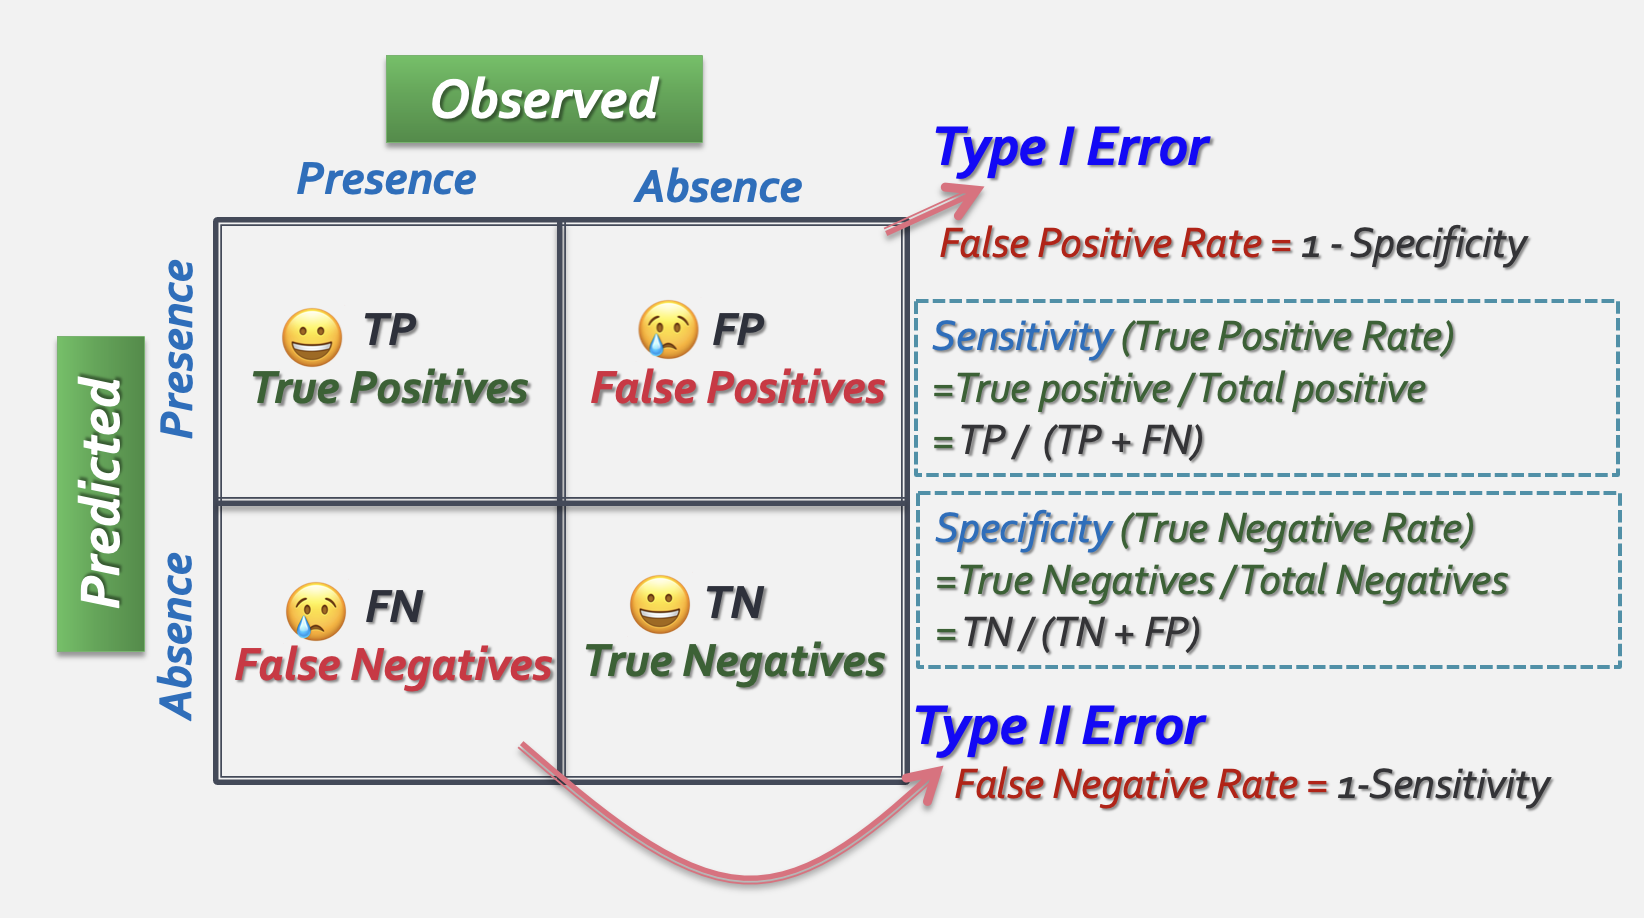
\includegraphics[width=0.7\textwidth]{cmx.png}
    \caption{Confusion Matrix: compares observed presence and absence records with predicted presence and absence records to measure multiple metrics representing accuracy of a model (e.g., sensitivity, specificity) }
    \label{fig:Fig3}
\end{figure}



\textbf{Description of the Metrics:}


- \uline{\textit{True Positives (TP)}}: The number of observed presences that are correctly predicted as presence by the model (i.e., the model correctly identifies the presence of the species).

- \uline{\textit{True Negatives (TN)}}: The number of observed absences that are correctly predicted as absence by the model (i.e., the model correctly identifies where the species is absent).
   
- \uline{\textit{False Negatives (FN)}}: The number of observed presences that are incorrectly predicted as absence (i.e., missed presences).

- \uline{\textit{False Positives (FP)}}: The number of absences where the model incorrectly predicts presence.


\textbf{Key Metrics Derived from the Confusion Matrix}:

- \uline{\textit{Accuracy}}: 
  \[
  \text{Accuracy} = \frac{TP + TN}{TP + TN + FP + FN}
  \]
\textbf{Accuracy} measures the overall correctness of the model by calculating the proportion of correctly classified instances (both presences and absences) out of all predictions.

- \uline{\textit{Sensitivity (True Positive Rate or Recall)}}:
  \[
  \text{Sensitivity} = \frac{TP}{TP + FN}
  \]
\textbf{Sensitivity} evaluates how well the model identifies actual presences (true positives). A higher sensitivity indicates fewer missed presences.

- \uline{\textit{Specificity (True Negative Rate)}}:
  \[
  \text{Specificity} = \frac{TN}{TN + FP}
  \]
\textbf{Specificity} assesses how well the model identifies actual absences (true negatives). A higher specificity means fewer false positives (wrongly predicted presences).

- \uline{\textit{Precision or ppv (Positive Predictive Value)}}:
  \[
  \text{Precision} = \frac{TP}{TP + FP}
  \]
\textbf{Precision} measures the proportion of predicted presences that are true presences. A higher precision means that when the model predicts presence, it is more likely to be correct.

- \uline{\textit{F1 Score}}:
  \[
  \text{F1 Score} = 2 \times \frac{\text{Precision} \times \text{Recall}}{\text{Precision} + \text{Recall}}
  \]
The \textbf{F1} score is the harmonic mean of precision and recall, giving a balanced measure of the model's accuracy when there is a trade-off between false positives and false negatives.


- \uline{\textit{Matthews Correlation Coefficient (MCC)}}:
  \[
  \text{MCC} = \frac{(TP \times TN) - (FP \times FN)}{\sqrt{(TP + FP)(TP + FN)(TN + FP)(TN + FN)}}
  \]

The \textbf{MCC} is a more balanced metric that considers all elements of the confusion matrix (TP, TN, FP, FN). It is particularly useful for imbalanced datasets, as it captures the relationship between true positives, true negatives, false positives, and false negatives. MCC ranges from -1 to 1, where 1 indicates perfect prediction, 0 means no better than random, and -1 means total disagreement between predictions and observations.

- \uline{\textit{True Skill Statistic or TSS}}:
  \[
  \text{TSS} = \text{Sensitivity} + \text{Specificity} - 1
  \]
    \textbf{TSS} is a widely used metric which evaluates model performance by combining sensitivity and specificity into a single measure. TSS ranges from -1 to 1, where 1 indicates perfect prediction, 0 indicates no better than random, and negative values indicate performance worse than random.


\textbf{Threshold Optimization}:

As mentioned, predictions from SDMs (those that are developed using presence-absence data) are in the form of probability (that may be interpreted as habitat suitability). Since probability values are not comparable with observed Presence/Absences, a threshold is needed to convert the probability values to presence-absences. Then, the question is that what is the best threshold! A threshold optimization method may be used to find the best threshold given some criteria available for this purpose. In the sdm R package, 15 different criteria are available (it can be specified in different functions through using the `opt` argument; check the help page of the `evaluates` function for more information). Here is a list of some widely used methods: 

For instance, we may find the threshold under which [sensitivity + specificity] is maximised (is known as: max[Se+Sp]).

Threshold optimization is crucial when converting continuous model predictions (e.g., probabilities of species presence) into binary classifications (presence/absence). Several approaches can be used for threshold optimization:

1) \uline{\textit{Se = Sp}}: This is one of the commonly used approach for threshold optimization, and it finds  the threshold where the sensitivity and specificity is equal. In the sdm package, this threshold can be used by setting `opt = 1`.

2) \uline{\textit{max[Se + Sp]}}: The is probably the most widely used approach, and it is the threshold that maximizes [sensitivity + specificity] which is equivalent to maximizing TSS. In the sdm package, this threshold can be used by setting `opt = 2` (default).

2) \uline{\textit{P10, P5, P1, and P0}}: These approached select the threshold based on percentile of probabilities across presence records in the evaluation dataset. P10, P5, P5, and P0 refer to 10, 5, 1, and 0 percentiles, respectively.


\textbf{\large Threshold-independent metrics}

The metrics mentioned so far are all threshold-based metrics, relying on finding the best threshold to first convert probability values to presence/absences, then creating a confusion matrix based on which multiple metrics can be calculated. Therefore, depending on which optimization approach is used, the metrics can vary. There is another group of metrics available to measure the performance of SDMs, with the advantage that there is no need to select a threshold. These threshold-independent metrics are often preferred when the goal is to evaluate the overall predictive ability of the model, regardless of specific classification cutoffs to convert probabilities to presence/absences.

- \uline{\textit{Area Under the Receiver Operating Characteristic Curve (AUC)}}: 

AUC (Area under the ROC curve) is probably the most widely used metric that measures the ability of SDMs to discriminate between presence and absence locations. AUC ranges between 0 and 1, with a value of 0.5 indicating a performance equivalent to random guessing, while values closer to 1 indicate better discriminative ability. AUC is calculated based on the ROC which plots the true positive rate (sensitivity) against the false positive rate (1-specificity) across all possible threshold values. AUC summarizes the curve into a single value, providing an overall assessment of model performance across thresholds.


\begin{figure}[H]
    \centering
    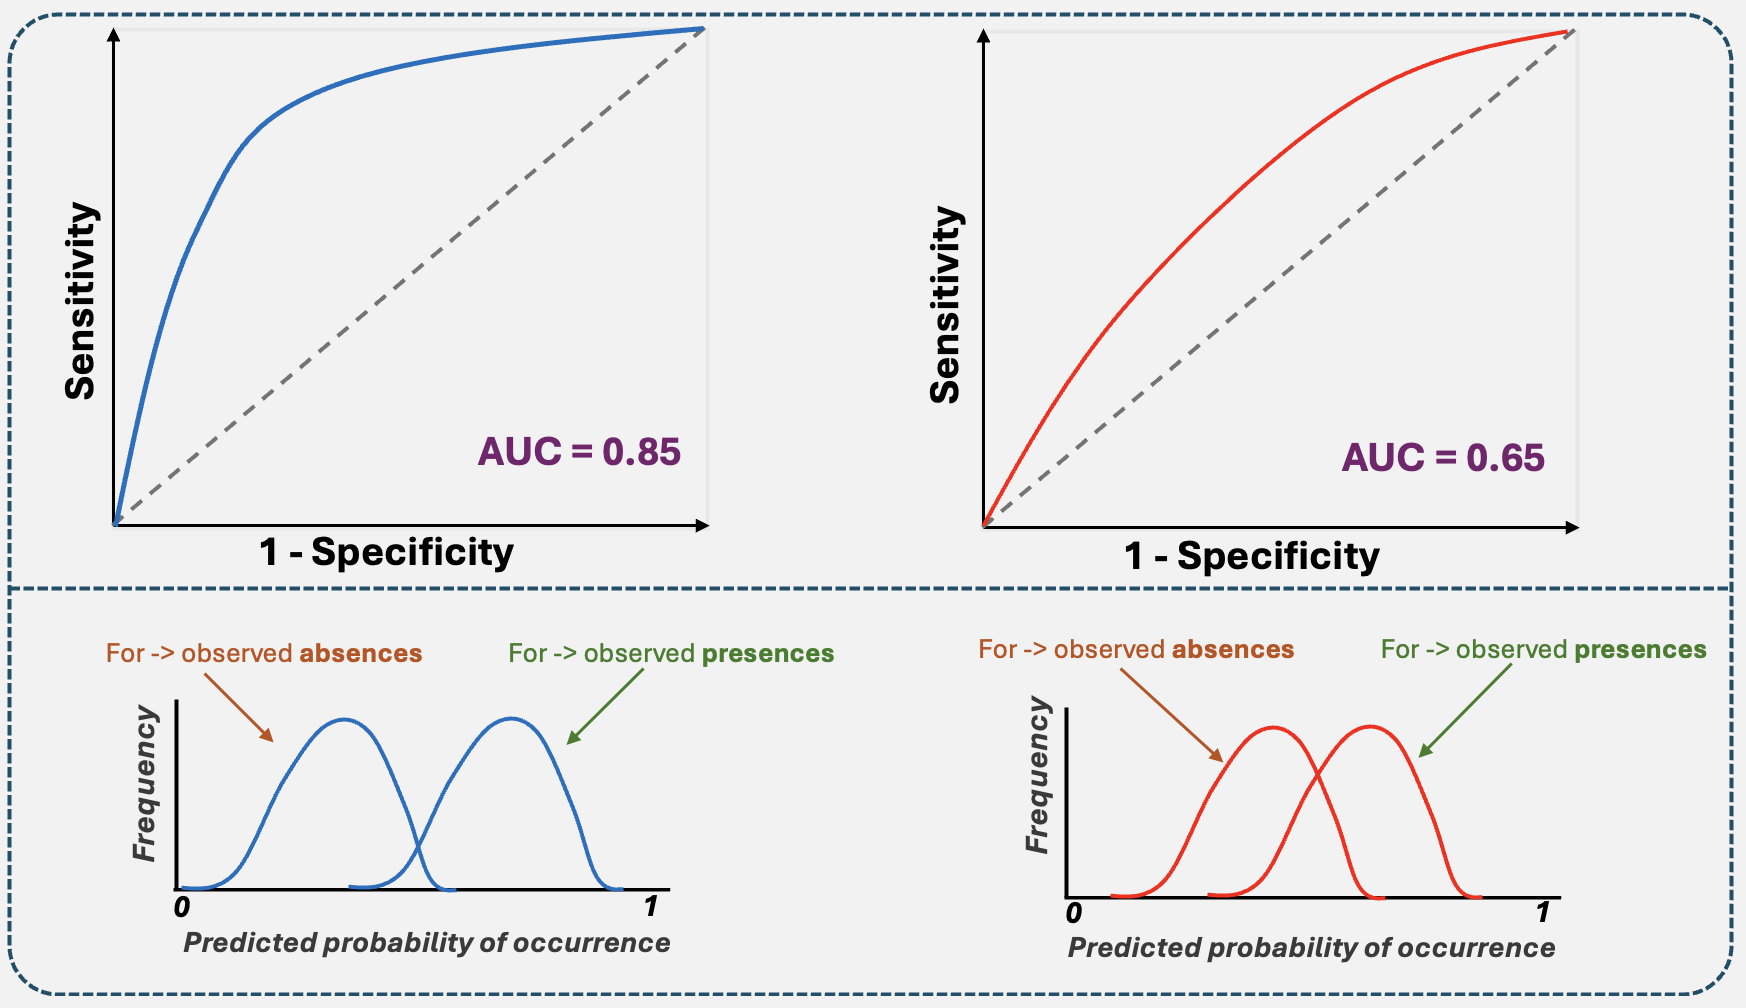
\includegraphics[width=0.75\textwidth]{roc.png}
    \caption{Two examples of ROC curve with corresponding AUC (area under the ROC curve) values; AUC is a metric assessing discriminative capacity of a model; the lower panel shows the density plots corresponding to the ROC curves in the upper panel, representing the distribution of predicted values across presence and absence locations in an evaluation (test) dataset; when AUC is greater, the model has greater power in discriminating presence locations from absence locations}
    \label{fig:Fig4}
\end{figure}

- \uline{\textit{Correlation (COR)}}: 

Correlation is another threshold-independent metric that assesses the agreement between predicted and observed values. The most common measure used is Pearson's correlation coefficient, which ranges from -1 to 1, with 1 showing a perfect positive correlation, 0 showing no correlation, and -1 representing perfect negative correlation.

- \uline{\textit{Devience}}: 

This metric represents the average deviation of model predictions from observations, therefore, a smaller value of it representing a better model (can be interpreted as smaller error).

- \uline{\textit{Continuous Boyce Index (CBI)}}: 

The Continuous Boyce Index (CBI) is an evaluation metric specifically designed for **presence-only** test dataset. It assesses how much better the predicted model is compared to a random model. CBI ranges from -1 to 1, where values close to 1 indicate a model with high predictive ability, 0 indicates no better than random, and negative values suggest the model is predicting worse than random.

- \uline{\textit{Calibration}}:

Calibration measures reliability of predicted probabilities related to observed species prevalence or proportion of presences across the range of probabilities predicted by a model.  If predictions are perfectly calibrated, we expect that the estimated probabilities represent the actual prevalence of data. For instance, across the sites with predicted probabiliy of 0.7, we expect 70% of observations are presence and 30% absence. The calibration metric is a novel method implemented in the sdm package to quantify the level of calibration, ranges between 0 and 1. A value of 1 refers to a perfect calibration and a value of 0.5 refers to the perfect discrimination (all observations greater than a threshold is presence, and below a threshold is absence). A negative value may also be generated for rare or not-likely situations such as generating opposite predictions (i.e., high probabilities for absences and low probabilities for presences). The following Figure shows a realistic calibration plot (on the left) with some extreme examples to show the range of calibration metrics (small plots on the right):

\begin{figure}[H]
    \centering
    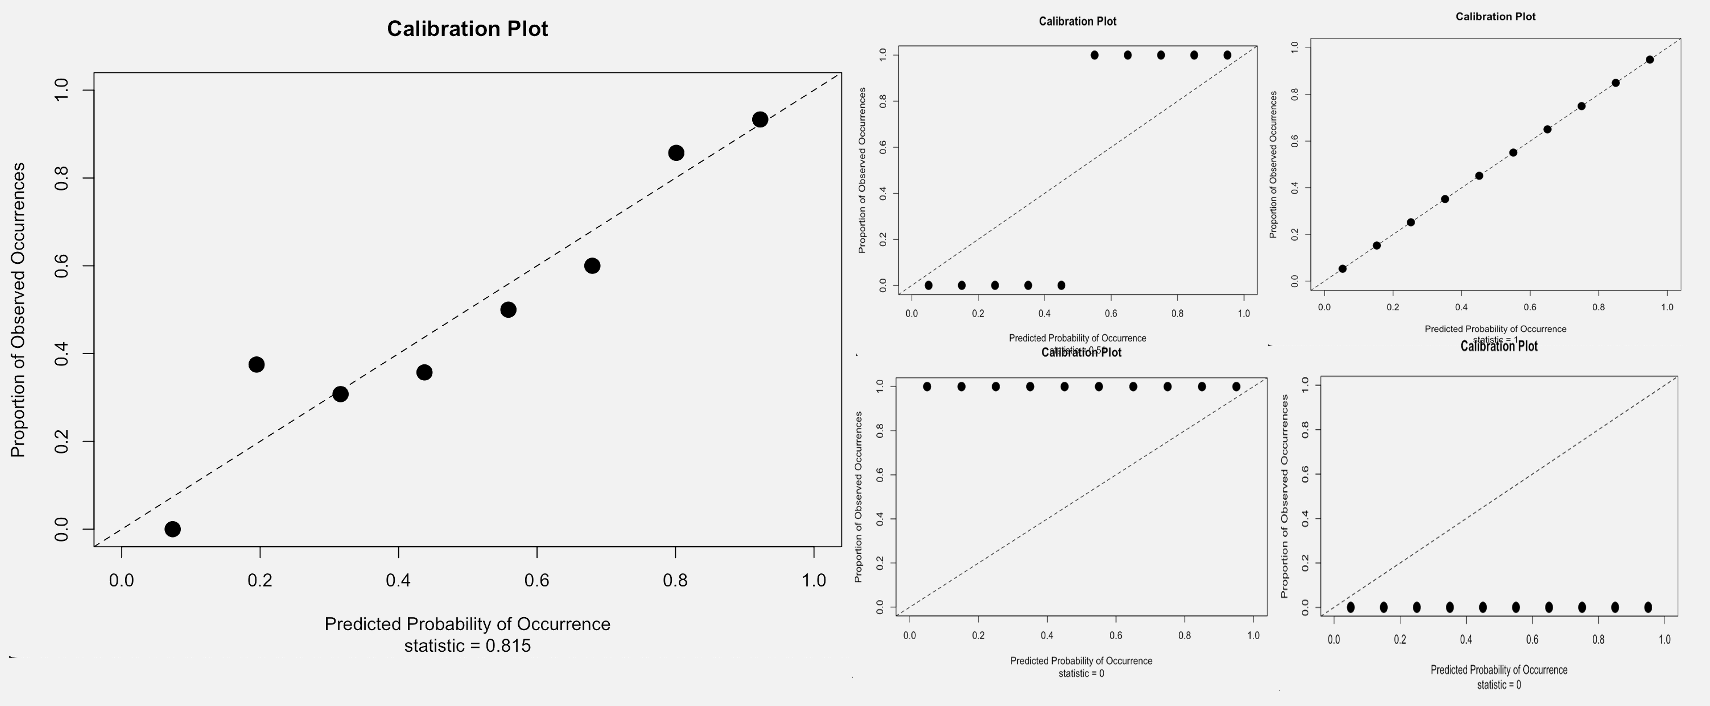
\includegraphics[width=0.75\textwidth]{calibration.png}
    \caption{The calibration plot with a novel metric developed in the sdm package representing the degree of calibration. The practical range is between 0.5 and 1.}
    \label{fig:Fig5}
\end{figure}



\end{mdframed}

\subsubsection{(iv) Predict/Project the map of habitat suitability in
current and future
times}\label{iv-predictproject-the-map-of-habitat-suitability-in-current-and-future-times}

After the models were trained and evaluated successfully, we can now use
them to predict the probability of occurrence (it may be interpreted as
the degree of habitat suitability) for each pixel across the study area.
Here, the aim is to assess the geographic distribution of the species
globally, therefore, we use the non-cropped predictor variables
(\texttt{bio}) to predict the values in the current time:

\begin{Shaded}
\begin{Highlighting}[]
\DocumentationTok{\#\# Predict habitat suitability of Snow leopard in the current time:}

\NormalTok{p }\OtherTok{\textless{}{-}} \FunctionTok{predict}\NormalTok{(m, bioc)}

\CommentTok{\# since we had 15 models in the \textasciigrave{}m\textasciigrave{} object, \textasciigrave{}p\textasciigrave{} is a SpatRaster with 15 layers }
\CommentTok{\# corresponding to the 15 models:}

\NormalTok{p}
\end{Highlighting}
\end{Shaded}

\begin{verbatim}
## class       : SpatRaster 
## dimensions  : 300, 360, 15  (nrow, ncol, nlyr)
## resolution  : 0.1666667, 0.1666667  (x, y)
## extent      : 60, 120, 10, 60  (xmin, xmax, ymin, ymax)
## coord. ref. : lon/lat WGS 84 (EPSG:4326) 
## source(s)   : memory
## names       :  id_1_~_subs,  id_2_~_subs,  id_3_~_subs, id_4_~_subs, id_5_~_subs, id_6_~_subs, ... 
## min values  : 2.220446e-16, 2.220446e-16, 1.079028e-13,  0.08533683,  0.08229015,  0.08046598, ... 
## max values  : 1.000000e+00, 1.000000e+00, 1.000000e+00,  0.72582535,  0.72132055,  0.71911020, ...
\end{verbatim}

\begin{Shaded}
\begin{Highlighting}[]
\CommentTok{\# We have 5 modelling methods, and 3 models for each method (15 in total),}
\CommentTok{\# the first 3 layers are for the first method ("glmp"), the secord 3 (4, 5, and 6)}
\CommentTok{\# are related to the second method ("brt"), and so on.}

\CommentTok{\# let\textquotesingle{}s visualise one of the outputs for each method:}

\CommentTok{\# appropriate color schemes:}
\NormalTok{cl }\OtherTok{\textless{}{-}} \FunctionTok{colorRampPalette}\NormalTok{(}\FunctionTok{c}\NormalTok{(}\StringTok{\textquotesingle{}gray\textquotesingle{}}\NormalTok{,}\StringTok{\textquotesingle{}orange\textquotesingle{}}\NormalTok{,}\StringTok{\textquotesingle{}yellow\textquotesingle{}}\NormalTok{,}\StringTok{\textquotesingle{}green\textquotesingle{}}\NormalTok{,}\StringTok{\textquotesingle{}blue\textquotesingle{}}\NormalTok{)) }

\DocumentationTok{\#\# rasterVis for visualisation:}
\CommentTok{\# So far, we used the simple plot function to visualise rasters,}
\CommentTok{\# but with rasterVis, you may generate nicer plots:}

\FunctionTok{library}\NormalTok{(rasterVis)}
\end{Highlighting}
\end{Shaded}

\begin{verbatim}
## Loading required package: lattice
\end{verbatim}

\begin{Shaded}
\begin{Highlighting}[]
\FunctionTok{levelplot}\NormalTok{(p[[}\FunctionTok{c}\NormalTok{(}\DecValTok{1}\NormalTok{,}\DecValTok{4}\NormalTok{,}\DecValTok{7}\NormalTok{,}\DecValTok{10}\NormalTok{,}\DecValTok{13}\NormalTok{)]],}\AttributeTok{col.regions=}\FunctionTok{cl}\NormalTok{(}\DecValTok{200}\NormalTok{),}\AttributeTok{margin=}\NormalTok{F)}
\end{Highlighting}
\end{Shaded}

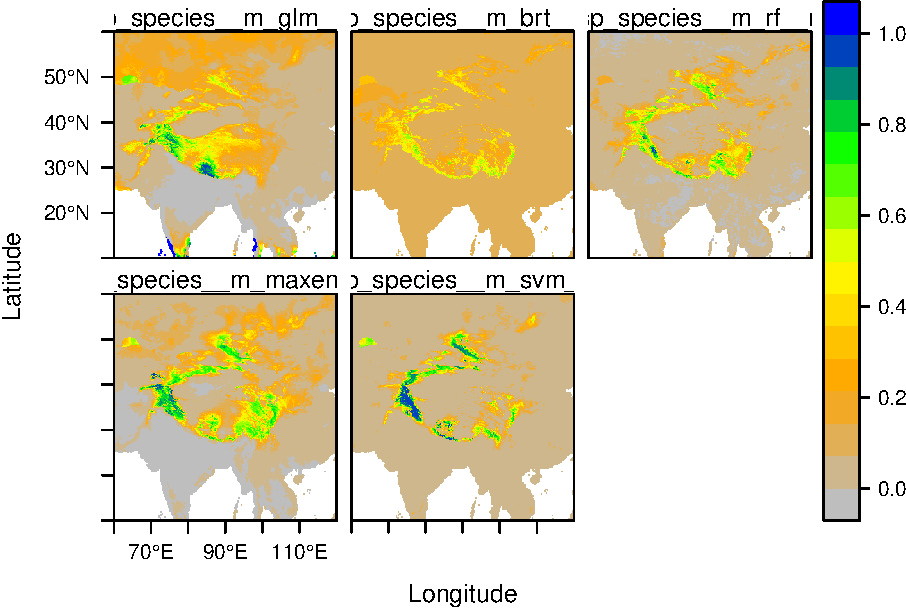
\includegraphics{sdm_R_files/figure-latex/unnamed-chunk-9-1.pdf}

\uline{\textit{Ensemble forecasting}}: Employing multiple modelling
methods for species distribution modelling which is usually applied to
several replications of data (e.g., in the example above, we produced 15
models), often results in varying predictions. While these models may
all perform well according to evaluation metrics (e.g., AUC), their
predictions can still differ significantly. These variations in outcomes
of models are referred to model-based uncertainty, which is one of the
key sources of uncertainty affecting SDMs.

To address this uncertainty, an effective approach is ensemble
forecasting, where the predictions from multiple models are combined
into a single, consensus prediction (Araujo and New 2007). Ensemble
forecasting helps to smooth out the variability in individual models,
providing a more robust and reliable prediction of species distribution.
According to Araújo and New (2007), ensemble methods can improve the
accuracy and reliability of SDMs by leveraging the strengths of
different models while minimizing their individual weaknesses.

\uline{\textit{Ensemble forecasting methods}}: In the sdm package, the
\texttt{ensemble} function can be used for generating the consensus
prediction that supports multiple methods for combining the predictions.
Several approaches are available to combine predictions from multiple
models in the \texttt{ensemble} function (the method is specified within
a list passed through the \texttt{setting} argument:

\begin{itemize}
\item
  \textbf{Mean} (simple averaging): This is the simplest method, where
  the predictions from all models are averaged to produce the final
  consensus prediction. Each model contributes equally to the final
  result. To use this method,
  \texttt{method\ =\ \textquotesingle{}mean\textquotesingle{}} or
  \texttt{method\ =\ \textquotesingle{}unweighted\textquotesingle{}} can
  be used in the \texttt{setting} argument of the \texttt{ensemble}
  function.
\item
  \textbf{Weighted Mean}: In this method, models with better performance
  (as determined by evaluation metrics such as AUC or TSS) are given
  more weight in the final prediction. For example, models that perform
  better based on AUC would contribute more significantly to the final
  ensemble prediction than models with lower AUC scores. Examples of
  settings in the \texttt{ensemble} function include:
  \texttt{setting\ =\ list(method\ =\ \textquotesingle{}weighted\textquotesingle{},\ stat\ =\ \textquotesingle{}auc\textquotesingle{})}
  which uses AUC values as weight; OR
  \texttt{setting\ =\ list(method\ =\ \textquotesingle{}weighted\textquotesingle{},\ stat\ =\ \textquotesingle{}tss\textquotesingle{},\ opt=2)}
  which uses TSS values as weight. Since TSS is a threshold-based
  metric, the \texttt{opt} argument is also added which specifies which
  threshold optimisation method should be used to select the best
  threshold for calculating TSS. 15 optimisation methods are available
  in the sdm package (check the help page of the \texttt{evaluates}
  function), and \texttt{opt\ =\ 2} refers to the second method that
  selects threshold under which {[}\texttt{sensitivity} +
  \texttt{specificity}{]} is maximized (i.e., \texttt{max{[}se+sp{]}}).
\item
  \textbf{Median}: This method takes the median of predictions from all
  models. To use this method
  (\texttt{method\ =\ \textquotesingle{}median\textquotesingle{}}).
\item
  \textbf{Thresholding and stacking}: This method involves thresholding
  predictions to determine areas of presence or absence given the best
  threshold for each model specified using a threshold optimisation
  method (the \texttt{opt} argument). The predicted presence-absence
  values from multiple models are stacked and averaged
  (\texttt{method\ =\ \textquotesingle{}pa\textquotesingle{}}). Example:
  \texttt{setting\ =\ list(method\ =\ \textquotesingle{}pa\textquotesingle{},\ opt=2)}
\item
  \textbf{Two-step averaging}: When multiple predictions are generated
  for each modelling method (from multiple data replications), the
  averaging of predictions can be done in two steps, across replications
  for each modelling method and then across modelling methods. The
  available two-step methods include \texttt{mean-weighted},
  \texttt{mean-unweighted}, \texttt{median-weighted} and
  \texttt{median-unweighted}. For instance, using the
  \texttt{method\ =\ \textquotesingle{}mean-weighted\textquotesingle{}}
  in the setting argument first takes the mean of different replications
  of each modelling methods, then they are combined through using a
  weighted-mean function.
\item
  \textbf{Assess variability in predictions}: In addition to generating
  a consensus prediction, several methods are avaialble to explore the
  variability of predictions for each location. These methods include
  coefficient of variation
  (\texttt{method\ =\ \textquotesingle{}cv\textquotesingle{}}), standard
  deviation
  (\texttt{method\ =\ \textquotesingle{}stdev\textquotesingle{}}),
  confidence interval
  (\texttt{method\ =\ \textquotesingle{}ci\textquotesingle{}}; this
  generates the range of confidence interval which is ``upper range -
  lower range''), and uncertainty
  (\texttt{method\ =\ \textquotesingle{}uncertainty\textquotesingle{}}).
  The uncertainty method can characterise model-based uncertainty or
  inconsistency among predictions of different models. An entropy metric
  is used to characterise uncertainty, ranging between 0 and 1. The
  value of 1 at a certain location refers to maximum inconsistency which
  is the case when half of the models predict `presence' for the
  location and the other half predict `absence'.
\end{itemize}

The above methods mentioned methods can be employed together at the same
time.

Following is examples of how to generate an ensemble prediction using
the \texttt{ensemble()} function in the sdm package. Please
\textbf{note} that the \texttt{ensemble} function
\uline{first calls the `predict` function to generate predictions}, and
then use an ensemble method to combine them into a consensus map.
However, if the predictions are generated beforehand, the output of the
predict function can be introduced as the second argument to the
ensemble function (in our case, \texttt{p}), otherwise, the predictors
object (in our case, \texttt{bioc}) should be used as the second
argument:

\begin{Shaded}
\begin{Highlighting}[]
\DocumentationTok{\#\# Ensemble:}
\CommentTok{\#{-}{-}{-}{-}\textgreater{} first argument: the model (output of the sdm function)}
\CommentTok{\#{-}{-}{-}{-}\textgreater{}  second argument: either the output of the predict function (if available)}
\CommentTok{\#{-}{-}{-}{-}{-}{-}{-}{-}{-}{-}{-}{-}{-}{-}{-}{-}{-}{-}{-}{-}{-}{-} OR the predictors object (bioc; )}
\CommentTok{\#{-}{-}{-}{-}\textgreater{} third argument (setting): a list with settings for ensemble procedure}

\DocumentationTok{\#\#\# We fitst try 3 methods and compare them in a plot:}

\DocumentationTok{\#\# (i) Weighted{-}mean using values of AUC as weights}
\NormalTok{en1 }\OtherTok{\textless{}{-}} \FunctionTok{ensemble}\NormalTok{(m, p, }\AttributeTok{setting =} \FunctionTok{list}\NormalTok{(}\AttributeTok{method=}\StringTok{\textquotesingle{}weighted\textquotesingle{}}\NormalTok{, }\AttributeTok{stat=} \StringTok{\textquotesingle{}auc\textquotesingle{}}\NormalTok{))}

\CommentTok{\#{-}{-}{-}{-}}
\DocumentationTok{\#\# (ii) Weighted{-}mean using values of TSS as weights }
\CommentTok{\# opt=2 refers to the threshold obtained using max[Sensitivity + Specificity]}

\NormalTok{en2 }\OtherTok{\textless{}{-}} \FunctionTok{ensemble}\NormalTok{(m, p, }\AttributeTok{setting =} \FunctionTok{list}\NormalTok{(}\AttributeTok{method=}\StringTok{\textquotesingle{}weighted\textquotesingle{}}\NormalTok{, }\AttributeTok{stat=} \StringTok{\textquotesingle{}tss\textquotesingle{}}\NormalTok{, }\AttributeTok{opt=}\DecValTok{2}\NormalTok{))}

\DocumentationTok{\#\# (iii) PA: thresholding and stacking:}
\NormalTok{en3 }\OtherTok{\textless{}{-}} \FunctionTok{ensemble}\NormalTok{(m, p, }\AttributeTok{setting =} \FunctionTok{list}\NormalTok{(}\AttributeTok{method=}\StringTok{\textquotesingle{}pa\textquotesingle{}}\NormalTok{, }\AttributeTok{opt=}\DecValTok{2}\NormalTok{))}

\CommentTok{\#{-}{-}{-}{-}{-}{-} }
\DocumentationTok{\#\# Visualising the outputs of 3 different ensembles:}


\NormalTok{en }\OtherTok{\textless{}{-}} \FunctionTok{c}\NormalTok{(en1,en2,en3) }\CommentTok{\# 3 objects stacked in a single object}
\FunctionTok{names}\NormalTok{(en) }\OtherTok{\textless{}{-}} \FunctionTok{c}\NormalTok{(}\StringTok{\textquotesingle{}ens\_AUC\textquotesingle{}}\NormalTok{,}\StringTok{\textquotesingle{}ens\_TSS\textquotesingle{}}\NormalTok{,}\StringTok{\textquotesingle{}ens\_PA\textquotesingle{}}\NormalTok{)}

\FunctionTok{levelplot}\NormalTok{(en,}\AttributeTok{col.regions=}\FunctionTok{cl}\NormalTok{(}\DecValTok{200}\NormalTok{),}\AttributeTok{margin=}\NormalTok{F,}
          \AttributeTok{main=}\FunctionTok{c}\NormalTok{(}\StringTok{\textquotesingle{}Weighted{-}Mean (AUC)\textquotesingle{}}\NormalTok{,}\StringTok{\textquotesingle{}Weighted{-}Mean (TSS)\textquotesingle{}}\NormalTok{,}\StringTok{\textquotesingle{}Thresholding (PA)\textquotesingle{}}\NormalTok{))}
\end{Highlighting}
\end{Shaded}

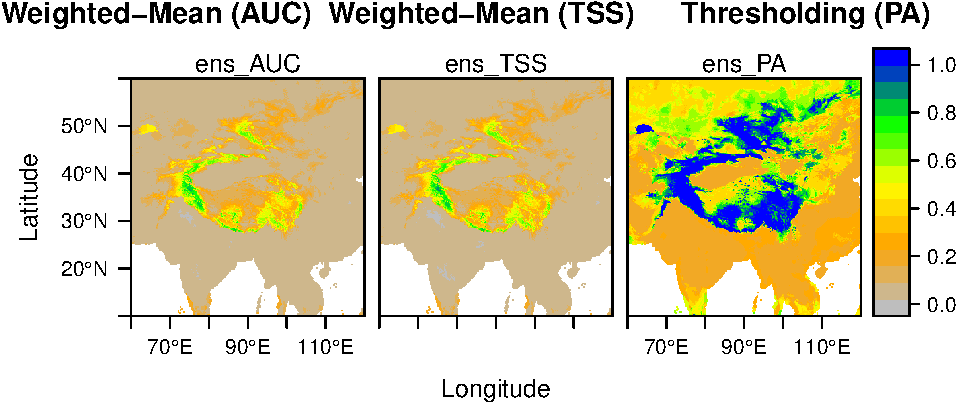
\includegraphics{sdm_R_files/figure-latex/unnamed-chunk-10-1.pdf}

\begin{Shaded}
\begin{Highlighting}[]
\CommentTok{\#{-}{-}{-}{-}{-}{-}{-}{-}{-}{-}{-}{-}{-}{-}{-}{-}{-}{-}{-}{-}{-}{-}{-}{-}{-}{-}{-}{-}{-}{-}{-}}
\DocumentationTok{\#\# Assessing variability among predictions:}

\NormalTok{en4 }\OtherTok{\textless{}{-}} \FunctionTok{ensemble}\NormalTok{(m, p, }\AttributeTok{setting =} \FunctionTok{list}\NormalTok{(}\AttributeTok{method=}\FunctionTok{c}\NormalTok{(}\StringTok{\textquotesingle{}mean\textquotesingle{}}\NormalTok{,}\StringTok{\textquotesingle{}ci\textquotesingle{}}\NormalTok{), }\AttributeTok{opt=}\DecValTok{2}\NormalTok{))}

\FunctionTok{levelplot}\NormalTok{(en4,}\AttributeTok{col.regions=}\FunctionTok{cl}\NormalTok{(}\DecValTok{200}\NormalTok{),}\AttributeTok{margin=}\NormalTok{F,}
          \AttributeTok{main=}\FunctionTok{c}\NormalTok{(}\StringTok{\textquotesingle{}Mean\textquotesingle{}}\NormalTok{,}\StringTok{\textquotesingle{}Range of Confidence{-}interval\textquotesingle{}}\NormalTok{))}
\end{Highlighting}
\end{Shaded}

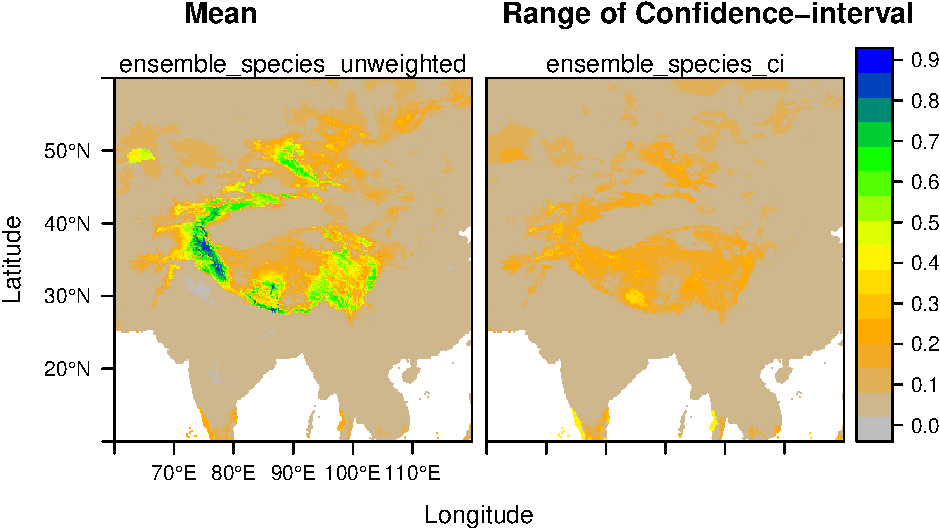
\includegraphics{sdm_R_files/figure-latex/unnamed-chunk-10-2.pdf}

\begin{Shaded}
\begin{Highlighting}[]
\DocumentationTok{\#\# to assess the upper and lower limits of confidence intervals:}
\NormalTok{ci.lower }\OtherTok{\textless{}{-}}\NormalTok{ en4[[}\DecValTok{1}\NormalTok{]] }\SpecialCharTok{{-}}\NormalTok{ (en4[[}\DecValTok{2}\NormalTok{]] }\SpecialCharTok{/} \DecValTok{2}\NormalTok{)}
\NormalTok{ci.upper }\OtherTok{\textless{}{-}}\NormalTok{ en4[[}\DecValTok{1}\NormalTok{]] }\SpecialCharTok{+}\NormalTok{ (en4[[}\DecValTok{2}\NormalTok{]] }\SpecialCharTok{/} \DecValTok{2}\NormalTok{)}
\NormalTok{ci }\OtherTok{\textless{}{-}} \FunctionTok{c}\NormalTok{(ci.lower,ci.upper)}
\FunctionTok{names}\NormalTok{(ci) }\OtherTok{\textless{}{-}} \FunctionTok{c}\NormalTok{(}\StringTok{\textquotesingle{}ci\_lower\textquotesingle{}}\NormalTok{,}\StringTok{\textquotesingle{}ci\_upper\textquotesingle{}}\NormalTok{)}

\FunctionTok{levelplot}\NormalTok{(ci,}\AttributeTok{margin=}\NormalTok{F,}
          \AttributeTok{main=}\FunctionTok{c}\NormalTok{(}\StringTok{\textquotesingle{}CI.lower (alpha = 0.05)\textquotesingle{}}\NormalTok{,}\StringTok{\textquotesingle{}CI.upper (alpha = 0.05)\textquotesingle{}}\NormalTok{))}
\end{Highlighting}
\end{Shaded}

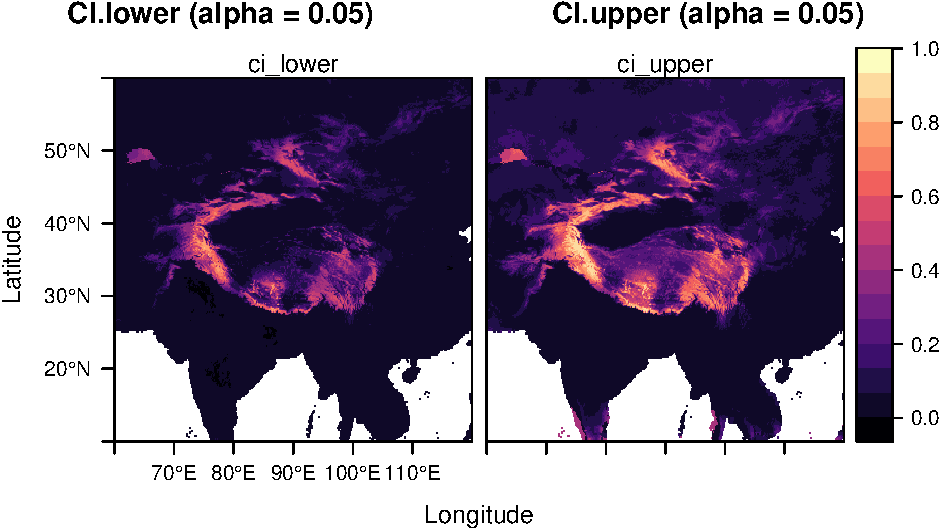
\includegraphics{sdm_R_files/figure-latex/unnamed-chunk-10-3.pdf}

\begin{Shaded}
\begin{Highlighting}[]
\CommentTok{\#{-}{-}{-}{-}{-}{-}{-}{-}{-}{-}}
\DocumentationTok{\#\# Uncertainty}
\NormalTok{en5 }\OtherTok{\textless{}{-}} \FunctionTok{ensemble}\NormalTok{(m, p, }\AttributeTok{setting =} \FunctionTok{list}\NormalTok{(}\AttributeTok{method=}\StringTok{\textquotesingle{}uncertainty\textquotesingle{}}\NormalTok{, }\AttributeTok{opt=}\DecValTok{2}\NormalTok{))}

\FunctionTok{levelplot}\NormalTok{(en5, }\AttributeTok{margin=}\NormalTok{F, }\AttributeTok{main=}\StringTok{\textquotesingle{}Model{-}based Uncertainty\textquotesingle{}}\NormalTok{)}
\end{Highlighting}
\end{Shaded}

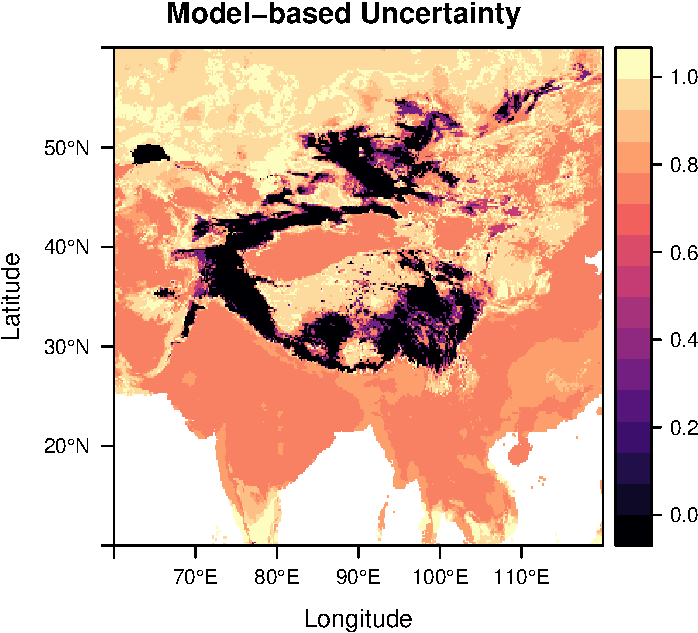
\includegraphics{sdm_R_files/figure-latex/unnamed-chunk-10-4.pdf}

As you can see above, a single map is generated by combining the 15
predicted rasters (output of the predict function) using the ensemble
method specified in the setting. There are other optional arguments
avaialable to control the ensemble procedure including:

\begin{itemize}
\item
  \texttt{id}: By default, predictions from all models are contributing
  to generate the consensus map unless a user specify the \texttt{id} of
  certain predictions (based on their \texttt{modelID}s). For example,
  adding \texttt{id\ =\ 1:10} to the \texttt{setting} list, only uses
  the first 10 predictions in the above example.
\item
  \texttt{expr}: An expression can be specified by a user to control or
  limit which predictions should contribute into generating the
  consensus map. For example, using
  \texttt{expr\ =\ auc\ \textgreater{}\ 0.7} uses the specified
  condition to only include well-performing models (those with AUC
  \textgreater{} 0.7) contributing to the ensemble procedure.
\item
  \texttt{power}: This argument is used to change weights by calculating
  \texttt{weights\ =\ weights\ \^{}\ power}. A value of greater than 1,
  gives more emphasise on better performing models.
\item
  Check the help page of the \texttt{ensemble} function in the
  \texttt{sdm} package for the other arguments and more details about
  the function.
\end{itemize}

\subsubsection{(v) Assessing range shifts of the species in response to
climate
change:}\label{v-assessing-range-shifts-of-the-species-in-response-to-climate-change}

In this section, the models are used to generate the spatial
distribution of species globally across time (i.e., for both the current
and future periods). SDMs can project potential changes in species'
geographic ranges by incorporating climate change scenarios (e.g.,
different future climate scenarios or SSPs). These projections allow
researchers to estimate how a species' suitable habitat might shift
under changing climate conditions.

\uline{\textit{Key Considerations for Assessing Range Shifts:}}:

\begin{enumerate}
\def\labelenumi{\alph{enumi})}
\item
  \textbf{Baseline Distribution vs.~Future Projections}: The first step
  in assessing range shifts involves comparing the baseline distribution
  of a species (i.e., its current range) with its projected distribution
  under future climate scenarios. These projections are typically made
  for various future time periods, such as 2050 or 2100 (here in this
  chapter, we only do it for the year 2100), based on different climate
  models (GCMs) and emission scenarios SSPs (Shared Socioeconomic
  Pathways). The difference between the two distributions highlights
  potential range expansions, contractions, or shifts.
\item
  \textbf{Types of Range Shifts}:
\end{enumerate}

\begin{itemize}
\item
  \textbf{Latitudinal Shifts}: Species may shift pole-ward in response
  to rising temperatures. For example, species in the northern
  hemisphere may move northward, while those in the southern hemisphere
  might shift southward.
\item
  \textbf{Altitudinal Shifts}: As temperatures increase, species living
  in mountainous regions may move to higher elevations where cooler
  conditions prevail.
\item
  \textbf{Range Contractions}: Some species might experience range
  contractions due to unsuitable environmental conditions, leading to
  local \textbf{extinctions}.
\item
  \textbf{Range Expansions}: Conversely, some species may benefit from
  climate change, expanding (colonizing) into new areas that were
  previously too cold or otherwise unsuitable.
\end{itemize}

\begin{enumerate}
\def\labelenumi{\alph{enumi})}
\setcounter{enumi}{2}
\tightlist
\item
  \textbf{Metrics for Quantifying Range Shifts}:
\end{enumerate}

\begin{itemize}
\item
  \textbf{Magnitude of Change}: The change in the degree of suitability
  between the future and current times can be simply calculated as a map
  by subtracting the current probability from the future one. Each pixel
  shows the magnitude of gains (positive values) and losses (negative
  values) in the future. Visualising the map highlights areas where
  habitat suitability increases (gain), decreases (loss), or remains
  unchanged. This can help to visualize the areas most affected by
  climate change. \[
     \text{Magnitude of Change} = \text{Habitat Suitability in Future} - \text{Habitat Suitability in Current}
     \]
\item
  \textbf{Assessing Expansion/Contraction}: By converting the habitat
  suitability values in both times to Presence/Absences, given a
  threshold, and comparing the values at each pixel, a pixel in future
  will be expanded (colonized) when species will be presence in the
  future while it is absence in the current time. Oppositely, the
  contraction (extinction) of a pixel in the future will be the case
  when species is presence in the current time wile it will become
  absence in the future.
\item
  \textbf{Centroid Shift}: The geographic centroid of the species' range
  is calculated for both the current and future projections. The
  distance and direction of the shift in the centroid can provide
  insight into whether the species is moving poleward, altitudinally, or
  in another direction. To calculate distance, we can use an Euclidean
  distance function (the coordinates should be metric): \[
     \text{Centroid shift} = \sqrt{(X_f - X_c)^2 + (Y_f - Y_c)^2}
     \] where \(X_f, Y_f\) represent the coordinates of the future
  centroid, and \(X_c, Y_c\) represent the current centroid coordinates.
\item
  \textbf{Range Overlap}: The degree of overlap between the current and
  future predicted range can be used to assess how much of the species'
  original habitat remains suitable under climate change. Low overlap
  indicates substantial changes in habitat suitability. \[
     \text{Range overlap (\%)} = \frac{\text{Area of overlap}}{\text{Current range area}} \times 100
     \]
\item
  \textbf{Range Area Change}: The change in the total area of suitable
  habitat is another key metric. This can be calculated by comparing the
  size of the species' predicted range in the future with its current
  range. \[
     \text{Range area change (\%)} = \frac{\text{Future range area} - \text{Current range area}}{\text{Current range area}} \times 100
     \]
\end{itemize}

\uline{\textit{Assessing Range Shifts for our case study}}:

For our case study, we have already fitted SDMs across a defined study
area, but now we want to use these models to predict the potential
distribution of the species \textbf{globally} for both the current and
future times. We have already downloaded bioclimatic data for both the
current period and future projections (year 2100 under the SSP585
scenario, which represents a high greenhouse gas emission scenario).
This will allow us to assess how the species' range might shift under a
potential future climate.

\textbf{Area of applicability}: Given that the SDMs were initially
fitted for a study area, which was a subset of the entire globe,
predicting across the global scale can introduce new challenges. When
applying these models globally, it is likely that some areas will
exhibit environmental conditions that were not represented within the
original study area. This phenomenon is referred to as environmental
extrapolation. It can affect the reliability of predictions and should
be carefully considered when interpreting the results. To handle this,
we can identify and restrict our predictions to areas where the
environmental conditions are within the area of applicability (AOA) of
the model, meaning that the conditions are similar to those found within
the training dataset. To calculate AOA, the \texttt{aoa} function in the
sdm package can be used which generates a raster map with pixel values
ranging between 0 and 1. A value of 1 means that the pixel is within the
range used to fit the model. Deviating from 1 toward 0 refers to a more
dissimilarity of the environmental condition of a pixel compared to the
condition used to fit SDMs.

Let's follow the range shift assessment globally step by step:

\begin{Shaded}
\begin{Highlighting}[]
\DocumentationTok{\#\# Predict spatial distribution for the current time (globally):}

\CommentTok{\# the model object: m, }
\CommentTok{\# the global bioclim dataset for the current time: bio}
\CommentTok{\# the global bioclim dataset for the current time: biof}

\CommentTok{\#{-}{-}{-}\textgreater{} we directly use the ensemble (no need to first run predict function):}
\CommentTok{\#{-}{-}{-}{-}{-}{-}\textgreater{} so, we use bio (predictors) as the second argument}

\NormalTok{hc }\OtherTok{\textless{}{-}} \FunctionTok{ensemble}\NormalTok{(m, bio, }\AttributeTok{setting=}\FunctionTok{list}\NormalTok{(}\AttributeTok{method=}\StringTok{"weighted"}\NormalTok{,}\AttributeTok{stat=}\StringTok{"auc"}\NormalTok{))}
\FunctionTok{names}\NormalTok{(hc) }\OtherTok{\textless{}{-}} \StringTok{\textquotesingle{}Current\textquotesingle{}}

\DocumentationTok{\#\# Project spatial distribution to the future}
\NormalTok{hf }\OtherTok{\textless{}{-}} \FunctionTok{ensemble}\NormalTok{(m, biof, }\AttributeTok{setting=}\FunctionTok{list}\NormalTok{(}\AttributeTok{method=}\StringTok{"weighted"}\NormalTok{,}\AttributeTok{stat=}\StringTok{"auc"}\NormalTok{))}
\FunctionTok{names}\NormalTok{(hf) }\OtherTok{\textless{}{-}} \StringTok{\textquotesingle{}Future\textquotesingle{}}

\NormalTok{cl }\OtherTok{\textless{}{-}} \FunctionTok{colorRampPalette}\NormalTok{(}\FunctionTok{c}\NormalTok{(}\StringTok{\textquotesingle{}gray\textquotesingle{}}\NormalTok{,}\StringTok{\textquotesingle{}orange\textquotesingle{}}\NormalTok{,}\StringTok{\textquotesingle{}yellow\textquotesingle{}}\NormalTok{,}\StringTok{\textquotesingle{}green\textquotesingle{}}\NormalTok{,}\StringTok{\textquotesingle{}blue\textquotesingle{}}\NormalTok{)) }


\FunctionTok{levelplot}\NormalTok{(}\FunctionTok{c}\NormalTok{(hc,hf),}\AttributeTok{col.regions=}\FunctionTok{cl}\NormalTok{(}\DecValTok{1000}\NormalTok{),}\AttributeTok{margin=}\NormalTok{F)}
\end{Highlighting}
\end{Shaded}

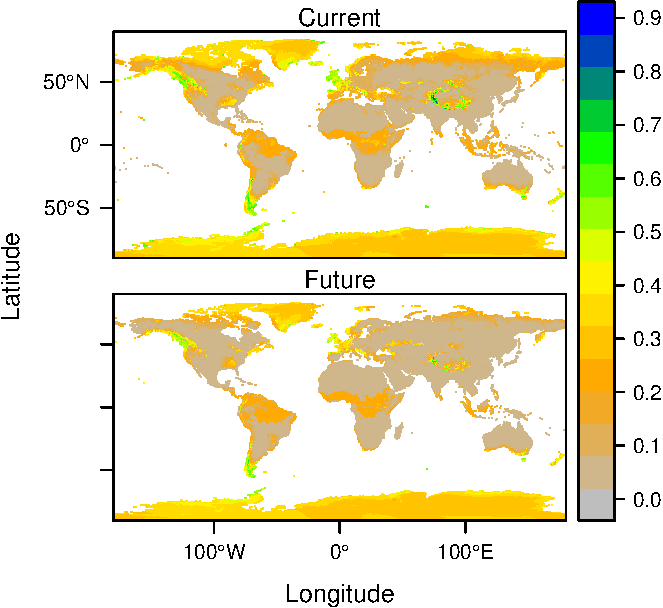
\includegraphics{sdm_R_files/figure-latex/unnamed-chunk-11-1.pdf}

\begin{Shaded}
\begin{Highlighting}[]
\DocumentationTok{\#\# Area of applicability:}

\CommentTok{\# to identify the unreliable pixels (check the Area of Applicability section):}
\CommentTok{\# The aoa function needs the following arguments:}
\CommentTok{\# {-}{-}{-}{-}\textgreater{} x: the raster predictors}
\CommentTok{\#{-}{-}{-}{-}{-}\textgreater{} d: the output of sdmData (or sdmModels)}
\CommentTok{\#{-}{-}{-}{-}{-}\textgreater{} vi: optional variable importance of the predictor variables}

\CommentTok{\#{-}{-} let\textquotesingle{}s first extract variable importance from the variables:}

\CommentTok{\# in the id argument, we may specify modelIDs or "ensemble":}
\NormalTok{vi }\OtherTok{\textless{}{-}} \FunctionTok{getVarImp}\NormalTok{(m,}\AttributeTok{id=}\StringTok{\textquotesingle{}ensemble\textquotesingle{}}\NormalTok{)}

\FunctionTok{plot}\NormalTok{(vi)}
\end{Highlighting}
\end{Shaded}

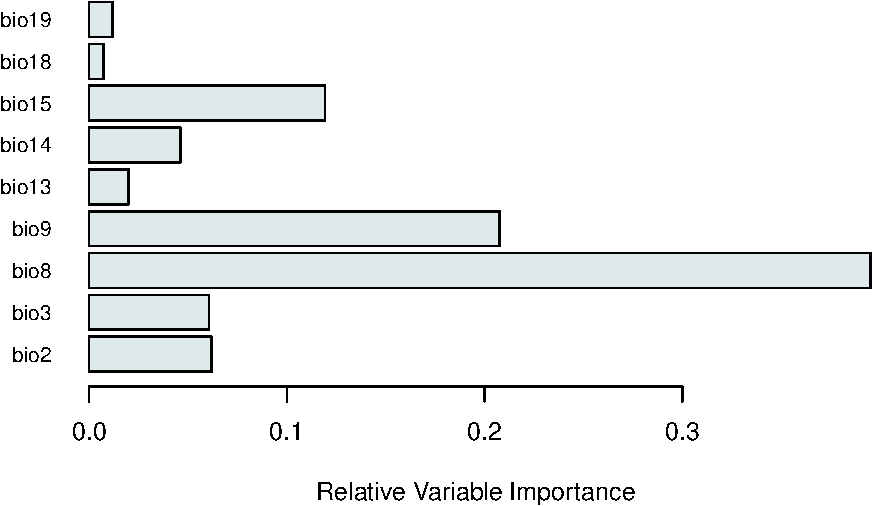
\includegraphics{sdm_R_files/figure-latex/unnamed-chunk-11-2.pdf}

\begin{Shaded}
\begin{Highlighting}[]
\NormalTok{vi}\SpecialCharTok{@}\NormalTok{varImportance}\SpecialCharTok{$}\NormalTok{corTest}
\end{Highlighting}
\end{Shaded}

\begin{verbatim}
## [1] 0.0619 0.0606 0.3951 0.2075 0.0200 0.0461 0.1193 0.0073 0.0119
\end{verbatim}

\begin{Shaded}
\begin{Highlighting}[]
\NormalTok{vimp }\OtherTok{\textless{}{-}}\NormalTok{ vi}\SpecialCharTok{@}\NormalTok{varImportance}\SpecialCharTok{$}\NormalTok{corTest }\CommentTok{\# get the vector of importances}

\NormalTok{ac }\OtherTok{\textless{}{-}} \FunctionTok{aoa}\NormalTok{(bio, m, }\AttributeTok{vi=}\NormalTok{vimp) }\CommentTok{\# the output is the raster layer (current time)}



\NormalTok{af }\OtherTok{\textless{}{-}} \FunctionTok{aoa}\NormalTok{(biof, m, }\AttributeTok{vi=}\NormalTok{vimp) }\CommentTok{\# for the future}

\CommentTok{\# let\textquotesingle{}s combine them into a single object for visualisation:}
\NormalTok{a }\OtherTok{\textless{}{-}} \FunctionTok{c}\NormalTok{(ac,af)}
\FunctionTok{names}\NormalTok{(a) }\OtherTok{\textless{}{-}} \FunctionTok{c}\NormalTok{(}\StringTok{\textquotesingle{}AOA\_current\textquotesingle{}}\NormalTok{,}\StringTok{\textquotesingle{}AOA\_future\textquotesingle{}}\NormalTok{)}

\FunctionTok{levelplot}\NormalTok{(a,}\AttributeTok{margin=}\NormalTok{F,}\AttributeTok{par.settings =}\NormalTok{ RdBuTheme)}
\end{Highlighting}
\end{Shaded}

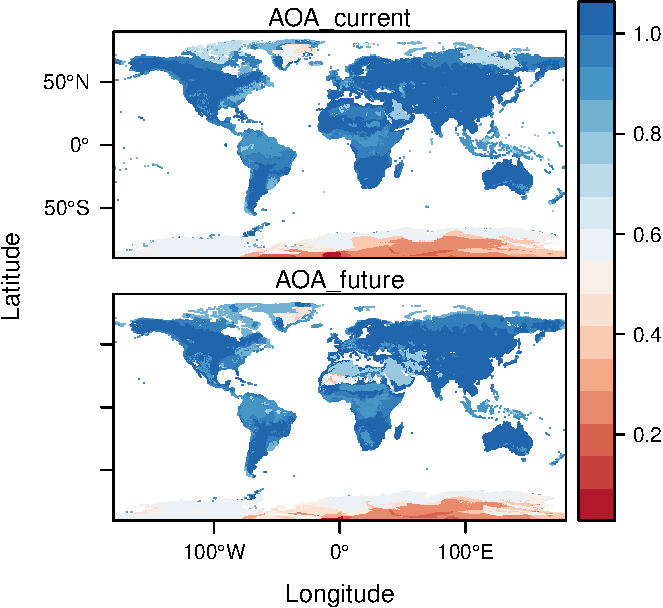
\includegraphics{sdm_R_files/figure-latex/unnamed-chunk-11-3.pdf}

\begin{Shaded}
\begin{Highlighting}[]
\CommentTok{\# the pixels less than 0.8 (or less than 1 to be conservative) are not reliable:}

\CommentTok{\# so, let\textquotesingle{}s make a mask:}

\NormalTok{acm }\OtherTok{\textless{}{-}} \FunctionTok{ifel}\NormalTok{(ac }\SpecialCharTok{\textgreater{}=} \FloatTok{0.8}\NormalTok{,}\DecValTok{1}\NormalTok{, }\ConstantTok{NA}\NormalTok{) }\CommentTok{\# a mask to only keep reliable pixels (current time)}
\NormalTok{afm }\OtherTok{\textless{}{-}} \FunctionTok{ifel}\NormalTok{(af }\SpecialCharTok{\textgreater{}=} \FloatTok{0.8}\NormalTok{,}\DecValTok{1}\NormalTok{, }\ConstantTok{NA}\NormalTok{) }\CommentTok{\# a mask to only keep reliable pixels (future time)}

\FunctionTok{plot}\NormalTok{(acm,}\AttributeTok{main=}\StringTok{\textquotesingle{}Mask of AoA for the current time\textquotesingle{}}\NormalTok{)}
\end{Highlighting}
\end{Shaded}

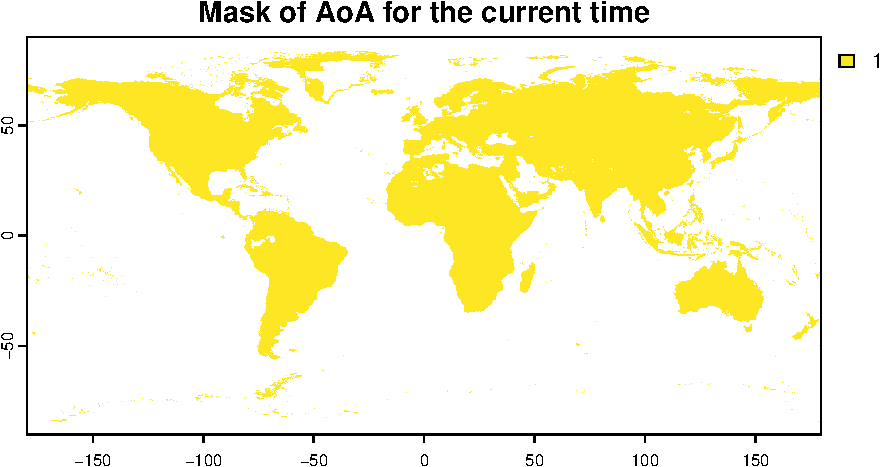
\includegraphics{sdm_R_files/figure-latex/unnamed-chunk-11-4.pdf}

\begin{Shaded}
\begin{Highlighting}[]
\CommentTok{\# let\textquotesingle{}s adjust the predictions/projections (hc, and hf):}

\NormalTok{hc }\OtherTok{\textless{}{-}} \FunctionTok{mask}\NormalTok{(hc, acm) }\CommentTok{\# exclude unreliable pixels for the current time}
\NormalTok{hf }\OtherTok{\textless{}{-}} \FunctionTok{mask}\NormalTok{(hf, afm) }\CommentTok{\# exclude unreliable pixels for the current time}

\FunctionTok{levelplot}\NormalTok{(}\FunctionTok{c}\NormalTok{(hc,hf),}\AttributeTok{col.regions=}\FunctionTok{cl}\NormalTok{(}\DecValTok{1000}\NormalTok{),}\AttributeTok{margin=}\NormalTok{F)}
\end{Highlighting}
\end{Shaded}

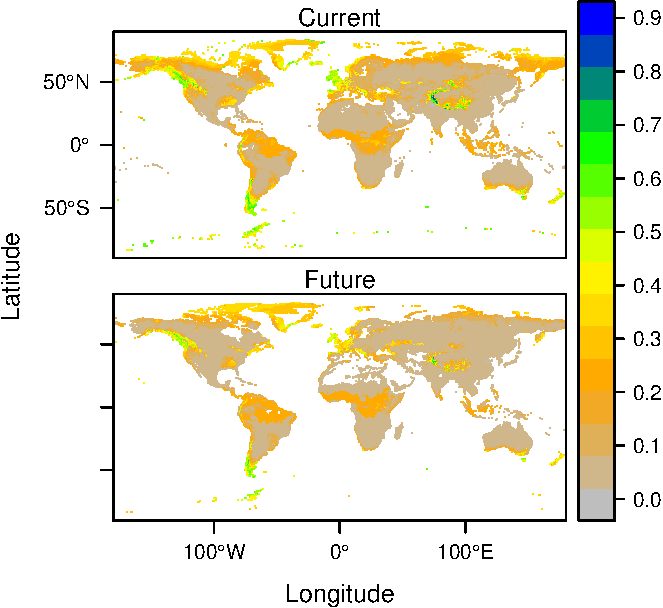
\includegraphics{sdm_R_files/figure-latex/unnamed-chunk-11-5.pdf}

\begin{Shaded}
\begin{Highlighting}[]
\DocumentationTok{\#\#{-}{-}{-}{-}{-}{-}{-}{-}{-}{-}{-}{-}{-}{-}{-}{-}{-}{-}{-}{-}{-}{-}{-}{-}{-}{-}{-}{-}{-}{-}{-}{-}{-}{-}{-}{-}{-}{-}{-}{-}{-}{-}{-}{-}{-}{-}{-}}

\DocumentationTok{\#\# Assess Magnitude of changes:}

\CommentTok{\# we can simply subtract current suitability from the future suitability:}

\NormalTok{ch }\OtherTok{\textless{}{-}}\NormalTok{ hf }\SpecialCharTok{{-}}\NormalTok{ hc}

\NormalTok{cl2 }\OtherTok{\textless{}{-}} \FunctionTok{colorRampPalette}\NormalTok{(}\FunctionTok{c}\NormalTok{(}\StringTok{\textquotesingle{}black\textquotesingle{}}\NormalTok{,}\StringTok{\textquotesingle{}darkred\textquotesingle{}}\NormalTok{,}\StringTok{\textquotesingle{}red\textquotesingle{}}\NormalTok{,}\StringTok{\textquotesingle{}orange\textquotesingle{}}\NormalTok{,}
                          \StringTok{\textquotesingle{}yellow\textquotesingle{}}\NormalTok{,}\StringTok{\textquotesingle{}gray\textquotesingle{}}\NormalTok{,}\StringTok{\textquotesingle{}blue\textquotesingle{}}\NormalTok{,}\StringTok{\textquotesingle{}darkblue\textquotesingle{}}\NormalTok{))}

\FunctionTok{levelplot}\NormalTok{(ch,}\AttributeTok{col.regions=}\FunctionTok{cl2}\NormalTok{(}\DecValTok{1000}\NormalTok{),}\AttributeTok{margin=}\NormalTok{F,}\AttributeTok{main=}\StringTok{\textquotesingle{}Magnitude of Gains/Losses\textquotesingle{}}\NormalTok{)}
\end{Highlighting}
\end{Shaded}

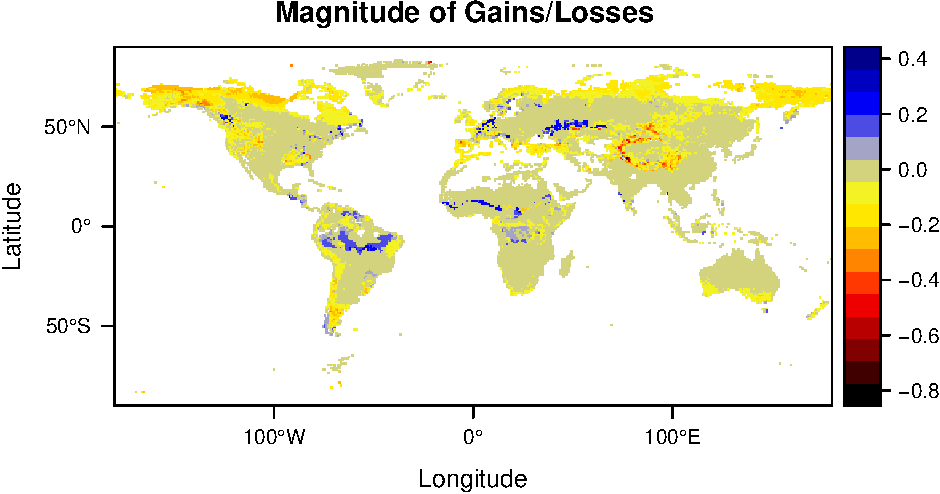
\includegraphics{sdm_R_files/figure-latex/unnamed-chunk-11-6.pdf}

\begin{Shaded}
\begin{Highlighting}[]
\DocumentationTok{\#\# Species range mapping and assess range shifts:}

\CommentTok{\# to map ranges, we can convert the habitat suitabilities to presence/absences (P/A)}
\CommentTok{\# the \textasciigrave{}pa\textasciigrave{} function can be used for this purpose:}
\CommentTok{\# pa uses a threshold to convert suitability values to P/As}

\CommentTok{\# to extract the threshold, we use the function of \textasciigrave{}threshold\textasciigrave{}:}
\CommentTok{\#{-}{-}{-} Arguments of getThreshold:}
\CommentTok{\#{-}{-}{-}{-}{-}{-}\textgreater{} x: sdmModels (m: output of the sdm function)}
\CommentTok{\#{-}{-}{-}{-}{-}{-}\textgreater{} id: From which model the threshold is extracted (it can be \textquotesingle{}ensemble\textquotesingle{})}
\CommentTok{\#{-}{-}{-}{-}{-}{-}\textgreater{} opt: which threshold optimisation method should be considered}
\CommentTok{\#{-}{-}{-}{-}{-}{-}\textgreater{} when id = "ensemble", we provide setting used for the ensemble function}


\NormalTok{th }\OtherTok{\textless{}{-}} \FunctionTok{getThreshold}\NormalTok{(m,}\AttributeTok{id=}\StringTok{\textquotesingle{}ensemble\textquotesingle{}}\NormalTok{,}\AttributeTok{opt=}\DecValTok{2}\NormalTok{,}\AttributeTok{setting=}\FunctionTok{list}\NormalTok{(}\AttributeTok{method=}\StringTok{\textquotesingle{}weighted\textquotesingle{}}\NormalTok{,}\AttributeTok{stat=}\StringTok{\textquotesingle{}auc\textquotesingle{}}\NormalTok{))}

\NormalTok{th }\CommentTok{\# the threshold to convert probability values to P/As using the \textasciigrave{}pa\textasciigrave{} function:}
\end{Highlighting}
\end{Shaded}

\begin{verbatim}
## [1] 0.30561
\end{verbatim}

\begin{Shaded}
\begin{Highlighting}[]
\CommentTok{\#{-}{-}{-} Arguments of pa:}
\CommentTok{\#{-}{-}{-}{-}{-}{-}\textgreater{} x: raster of habitat suitability}
\CommentTok{\#{-}{-}{-}{-}{-}{-}\textgreater{} y: threshold value}

\NormalTok{pac }\OtherTok{\textless{}{-}} \FunctionTok{pa}\NormalTok{(hc, th) }\CommentTok{\# P/As for the current time (baseline)}

\NormalTok{paf }\OtherTok{\textless{}{-}} \FunctionTok{pa}\NormalTok{(hf, th) }\CommentTok{\# P/As for the future time}

\CommentTok{\#{-}{-}{-}{-}{-}{-}{-}{-}{-}{-}{-}{-}{-}}
\CommentTok{\# let\textquotesingle{}s visualise them:}

\CommentTok{\# defining a colorKey for the legend in map:}
\NormalTok{colKey }\OtherTok{\textless{}{-}} \FunctionTok{list}\NormalTok{(}\AttributeTok{at=}\FunctionTok{c}\NormalTok{(}\DecValTok{0}\NormalTok{,}\FloatTok{0.5}\NormalTok{,}\DecValTok{1}\NormalTok{), }\DocumentationTok{\#\# where the colors change in legend}
                   \AttributeTok{labels=}\FunctionTok{list}\NormalTok{(}
                     \AttributeTok{at=}\FunctionTok{c}\NormalTok{(}\DecValTok{0}\NormalTok{,}\DecValTok{1}\NormalTok{) }\DocumentationTok{\#\# where to print labels}
\NormalTok{                   ))}

\FunctionTok{levelplot}\NormalTok{(}\FunctionTok{c}\NormalTok{(pac,paf),}\AttributeTok{col.regions=}\FunctionTok{c}\NormalTok{(}\StringTok{\textquotesingle{}gray\textquotesingle{}}\NormalTok{,}\StringTok{\textquotesingle{}green\textquotesingle{}}\NormalTok{),}\AttributeTok{margin=}\NormalTok{F,}\AttributeTok{colorkey=}\NormalTok{colKey)}
\end{Highlighting}
\end{Shaded}

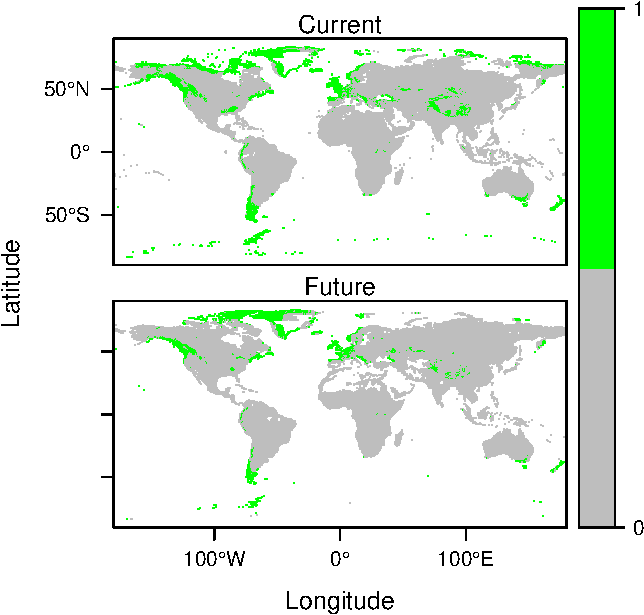
\includegraphics{sdm_R_files/figure-latex/unnamed-chunk-11-7.pdf}

\begin{Shaded}
\begin{Highlighting}[]
\CommentTok{\#{-}{-}{-}{-}{-}{-}{-}{-}{-}{-}{-}{-}{-}{-}{-}{-}{-}{-}{-}{-}{-}{-}{-}}

\DocumentationTok{\#\# Range shift metrics:}

\CommentTok{\# by subtracting the current P/As from the future one, we can get the following}
\CommentTok{\# values in the map:}

\CommentTok{\#{-}{-}{-}{-}{-}{-}{-}{-}{-}{-}{-}{-}{-}{-}{-}{-}{-}{-}{-}{-}{-}{-}{-}{-}{-}{-}}
\CommentTok{\# Future {-} Current = Change}
\CommentTok{\#{-}{-}{-}{-}{-}{-}{-}{-}{-}{-}{-}{-}{-}{-}{-}{-}{-}{-}{-}{-}{-}{-}{-}{-}{-}{-}}
\CommentTok{\#   1    {-}   0     = 1; Expansion (P in future; A in current)}
\CommentTok{\#   1    {-}   1     = 0; No Change; persistence (P in future; P in current)}
\CommentTok{\#   0    {-}   0     = 0; No Change; Unsuitable (A in; A in current)}
\CommentTok{\#   0    {-}   1     = {-}1; Contraction or Extinction (A in future; P in current)}

\CommentTok{\#{-}{-}{-}{-}{-}{-}{-}{-}{-}{-}{-}{-}{-}{-}{-}{-}{-}{-}{-}{-}{-}{-}{-}{-}{-}{-}{-}}

\CommentTok{\# As you can see above, No change in suitable and unsuitable sites can not be }
\CommentTok{\# separated, a solution can be to change the 1/0 values in the future layer to }
\CommentTok{\# a different value, e.g., 100/0 (so, presence sites in the future layer has a }
\CommentTok{\# value of 100)! To do so, we can simply multiply paf to 100:}

\NormalTok{paf2 }\OtherTok{\textless{}{-}}\NormalTok{ paf }\SpecialCharTok{*} \DecValTok{100} 

\CommentTok{\# Now:}
\CommentTok{\#{-}{-}{-}{-}{-}{-}{-}{-}{-}{-}{-}{-}{-}{-}{-}{-}{-}{-}{-}{-}{-}{-}{-}{-}{-}{-}}
\CommentTok{\# Future {-} Current = Change}
\CommentTok{\#{-}{-}{-}{-}{-}{-}{-}{-}{-}{-}{-}{-}{-}{-}{-}{-}{-}{-}{-}{-}{-}{-}{-}{-}{-}{-}}
\CommentTok{\#   100   {-}   0    = 100; Expansion (P in future; A in current)}
\CommentTok{\#   100   {-}   1    = 99; No Change; Refugia (P in future; P in current)}
\CommentTok{\#   0     {-}   0    = 0; No Change; Unsuitable (A in; A in current)}
\CommentTok{\#   0     {-}   1    = {-}1; Contraction or Extinction (A in future; P in current)}

\CommentTok{\#{-}{-}{-}{-}{-}{-}{-}{-}{-}{-}{-}{-}{-}{-}{-}{-}{-}{-}{-}{-}{-}{-}{-}{-}{-}{-}{-}}
\CommentTok{\# so, we have 4 possible values representing range shifts}

\NormalTok{pach }\OtherTok{\textless{}{-}}\NormalTok{ paf2 }\SpecialCharTok{{-}}\NormalTok{ pac}


\NormalTok{cls }\OtherTok{\textless{}{-}} \FunctionTok{data.frame}\NormalTok{(}\AttributeTok{id=}\FunctionTok{c}\NormalTok{(}\SpecialCharTok{{-}}\DecValTok{1}\NormalTok{,}\DecValTok{0}\NormalTok{,}\DecValTok{99}\NormalTok{,}\DecValTok{100}\NormalTok{), }
                  \AttributeTok{range=}\FunctionTok{c}\NormalTok{(}\StringTok{\textquotesingle{}Extinction\textquotesingle{}}\NormalTok{, }\StringTok{\textquotesingle{}Unsuitable\_NoChange\textquotesingle{}}\NormalTok{, }
                          \StringTok{\textquotesingle{}Refugia\textquotesingle{}}\NormalTok{,}\StringTok{\textquotesingle{}Expansion\textquotesingle{}}\NormalTok{))}

\FunctionTok{levels}\NormalTok{(pach) }\OtherTok{\textless{}{-}}\NormalTok{ cls}


\FunctionTok{levelplot}\NormalTok{(pach,}\AttributeTok{att=}\StringTok{\textquotesingle{}range\textquotesingle{}}\NormalTok{,}\AttributeTok{col.regions=}\FunctionTok{c}\NormalTok{(}\StringTok{\textquotesingle{}red\textquotesingle{}}\NormalTok{,}\StringTok{\textquotesingle{}gray\textquotesingle{}}\NormalTok{,}\StringTok{\textquotesingle{}green\textquotesingle{}}\NormalTok{,}\StringTok{\textquotesingle{}blue\textquotesingle{}}\NormalTok{),}\AttributeTok{margin=}\NormalTok{F)}
\end{Highlighting}
\end{Shaded}

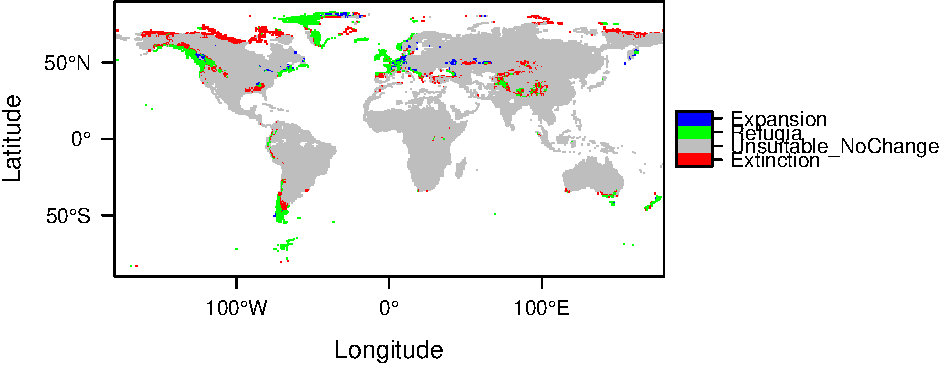
\includegraphics{sdm_R_files/figure-latex/unnamed-chunk-11-8.pdf}

\begin{Shaded}
\begin{Highlighting}[]
\CommentTok{\# Refugia is important for biodiversity conservation as it indicates potential }
\CommentTok{\# locations for species to persist amid climate change, These locations enhance }
\CommentTok{\# the likelihood of survival for species during climate shifts.}

\DocumentationTok{\#\#{-}{-}{-}{-}{-}{-}{-}{-}{-}{-}{-}{-}{-}{-}{-}{-}{-}{-}{-}{-}{-}{-}{-}{-}{-}{-}{-}{-}{-}{-}{-}{-}{-}{-}{-}{-}{-}{-}}

\DocumentationTok{\#\# Metrics of Range Shift assessment:}
\DocumentationTok{\#\#{-}{-}{-}{-}{-}{-}{-}{-}{-}{-}{-}{-}{-}{-}{-}{-}{-}{-}{-}{-}{-}{-}{-}{-}{-}{-}{-}{-}{-}{-}{-}{-}{-}{-}}

\CommentTok{\# Here, we quantitatively assess range shifts:}

\DocumentationTok{\#\# Area of Contraction (Extinction) and Expansion (Colonization):}
\CommentTok{\# to calculate the area of the pixels representing either of the contraction}
\CommentTok{\# or expansion classes, we first need to identify the pixels of these classes}

\CommentTok{\# By multiplying the number of pixels of each class to the area/size of a pixel,}
\CommentTok{\# we may roughly estimate the area, however, since our dataset uses a lat/lon}
\CommentTok{\# coordinate reference system, the area of pixels are varying across latitudes,}
\CommentTok{\# therefore, we may first calculate the area of each pixel, and then use the areas}
\CommentTok{\# to calculate the size of contraction or expansion:}

\CommentTok{\# we can use the cellSize function to measure the size of pixels:}
\NormalTok{area }\OtherTok{\textless{}{-}} \FunctionTok{cellSize}\NormalTok{(pach, }\AttributeTok{unit=}\StringTok{\textquotesingle{}km\textquotesingle{}}\NormalTok{) }\CommentTok{\# a raster with areas assigned to pixels}

\CommentTok{\# which cells belong to the class of contraction?}
\CommentTok{\# in pach, the value of {-}1 represents contraction (extinction):}

\NormalTok{w1 }\OtherTok{\textless{}{-}} \FunctionTok{which}\NormalTok{(pach[] }\SpecialCharTok{==} \SpecialCharTok{{-}}\DecValTok{1}\NormalTok{) }\CommentTok{\# which cells in pach has the value of {-}1 (extinction)?}

\FunctionTok{head}\NormalTok{(w1) }\CommentTok{\# w1 is a vector with cell numbers of pixels for the class of extinction}
\end{Highlighting}
\end{Shaded}

\begin{verbatim}
## [1] 82972 82973 82974 82975 82976 82977
\end{verbatim}

\begin{Shaded}
\begin{Highlighting}[]
\FunctionTok{sum}\NormalTok{(area[w1]) }\CommentTok{\# Area of Extinction (km2) in the year 2100 based on SSP5 scenario!}
\end{Highlighting}
\end{Shaded}

\begin{verbatim}
## [1] 5398468
\end{verbatim}

\begin{Shaded}
\begin{Highlighting}[]
\NormalTok{w2 }\OtherTok{\textless{}{-}} \FunctionTok{which}\NormalTok{(pach[] }\SpecialCharTok{==} \DecValTok{100}\NormalTok{) }\CommentTok{\# which cells in pach has the value of 100 (expansion)?}

\FunctionTok{sum}\NormalTok{(area[w2]) }\CommentTok{\# Area of Expansion (km2) in the year 2100 based on SSP5 scenario!}
\end{Highlighting}
\end{Shaded}

\begin{verbatim}
## [1] 947459
\end{verbatim}

\begin{Shaded}
\begin{Highlighting}[]
\DocumentationTok{\#\#\#\#\#\#\#\#\#\#\#\#\#\#\#\#\#\#\#\#\#\#\#\#\#\#\#\#\#}
\DocumentationTok{\#\# Calculate centroid shift:}

\CommentTok{\# to calculate centroid shift, we need to first calculate Xf,Xc, Yf, and Yc which }
\CommentTok{\# are the mean X and Y (longitudes and latitudes) across pixels of species range }
\CommentTok{\# in the Current (c) and Future times (f)}

\CommentTok{\# Let\textquotesingle{}s first identify cells of species range for the current and future time}

\CommentTok{\# which pixels in pac (presence/ansence of current time) is equal to 1?}
\NormalTok{Wc }\OtherTok{\textless{}{-}} \FunctionTok{which}\NormalTok{(pac[] }\SpecialCharTok{==} \DecValTok{1}\NormalTok{) }\CommentTok{\# pixel numbers of species range in the current time}
\NormalTok{Wf }\OtherTok{\textless{}{-}} \FunctionTok{which}\NormalTok{(paf[] }\SpecialCharTok{==} \DecValTok{1}\NormalTok{) }\CommentTok{\# pixel number of species range in the future time}

\NormalTok{XYc }\OtherTok{\textless{}{-}} \FunctionTok{xyFromCell}\NormalTok{(pac, Wc)}\CommentTok{\# X and Y coordinates of the current time across Wc cells}
\NormalTok{XYf }\OtherTok{\textless{}{-}} \FunctionTok{xyFromCell}\NormalTok{(paf, Wf)}\CommentTok{\# X and Y coordinates of the future time across Wf cells}


\FunctionTok{head}\NormalTok{(XYc) }\CommentTok{\# let\textquotesingle{}s see how they look like}
\end{Highlighting}
\end{Shaded}

\begin{verbatim}
##              x        y
## [1,] -38.91667 83.58333
## [2,] -38.75000 83.58333
## [3,] -38.58333 83.58333
## [4,] -38.41667 83.58333
## [5,] -37.58333 83.58333
## [6,] -37.41667 83.58333
\end{verbatim}

\begin{Shaded}
\begin{Highlighting}[]
\NormalTok{Xc }\OtherTok{\textless{}{-}} \FunctionTok{mean}\NormalTok{(XYc[,}\DecValTok{1}\NormalTok{],}\AttributeTok{na.rm=}\NormalTok{T) }\CommentTok{\# mean of the X column}
\NormalTok{Yc }\OtherTok{\textless{}{-}} \FunctionTok{mean}\NormalTok{(XYc[,}\DecValTok{2}\NormalTok{],}\AttributeTok{na.rm=}\NormalTok{T) }\CommentTok{\# mean of the Y column}

\NormalTok{Xf }\OtherTok{\textless{}{-}} \FunctionTok{mean}\NormalTok{(XYf[,}\DecValTok{1}\NormalTok{],}\AttributeTok{na.rm=}\NormalTok{T) }
\NormalTok{Yf }\OtherTok{\textless{}{-}} \FunctionTok{mean}\NormalTok{(XYf[,}\DecValTok{2}\NormalTok{],}\AttributeTok{na.rm=}\NormalTok{T) }

\NormalTok{Xc}
\end{Highlighting}
\end{Shaded}

\begin{verbatim}
## [1] -27.3959
\end{verbatim}

\begin{Shaded}
\begin{Highlighting}[]
\NormalTok{Yc}
\end{Highlighting}
\end{Shaded}

\begin{verbatim}
## [1] 41.37305
\end{verbatim}

\begin{Shaded}
\begin{Highlighting}[]
\NormalTok{Xf}
\end{Highlighting}
\end{Shaded}

\begin{verbatim}
## [1] -37.26772
\end{verbatim}

\begin{Shaded}
\begin{Highlighting}[]
\NormalTok{Yf}
\end{Highlighting}
\end{Shaded}

\begin{verbatim}
## [1] 44.43572
\end{verbatim}

\begin{Shaded}
\begin{Highlighting}[]
\CommentTok{\# We can calculate Euclidean distance to measure the shift distance between the }
\CommentTok{\# future and  current times. However, since the coordinate reference system (CRS) }
\CommentTok{\# of our layers is geographic, the coordinates of the centroids are also }
\CommentTok{\# in the unit of decimal degrees (based on latlon CRS). To calculate distance in}
\CommentTok{\# meter, we can use the distGeo function from the package of geosphere }
\CommentTok{\# to calculate metric distance between two points when they are in geographic }
\CommentTok{\# coordinates.}

\CommentTok{\# To do so, first let\textquotesingle{}s load the geosphere package (install it if you don\textquotesingle{}t have it)}
\FunctionTok{library}\NormalTok{(geosphere)}

\CommentTok{\# distance between two points (centroids) based on their coordinates:}
\NormalTok{dis }\OtherTok{\textless{}{-}} \FunctionTok{distGeo}\NormalTok{(}\FunctionTok{c}\NormalTok{(Xc,Yc),}\FunctionTok{c}\NormalTok{(Xf,Yf)) }\SpecialCharTok{/} \DecValTok{1000} \CommentTok{\# divided by 1000 to get distance in KM}


\NormalTok{dis}
\end{Highlighting}
\end{Shaded}

\begin{verbatim}
## [1] 874.3126
\end{verbatim}

\begin{Shaded}
\begin{Highlighting}[]
\DocumentationTok{\#\# Direction of change:}

\CommentTok{\# we can use the bearing (from the geosphere package) function to get the }
\CommentTok{\# azimut (direction) from the centroind of current time to the future:}


\NormalTok{azimuth\_deg }\OtherTok{\textless{}{-}} \FunctionTok{bearing}\NormalTok{(}\FunctionTok{c}\NormalTok{(Xc,Yc),}\FunctionTok{c}\NormalTok{(Xf,Yf))}

\CommentTok{\# we can convert it to a range between 0 to 360 to get}
\CommentTok{\# a clockwise direction{-}{-}\textgreater{} 0: north; 90: west, 180: south; 270: west; 360: north}

\ControlFlowTok{if}\NormalTok{ (azimuth\_deg }\SpecialCharTok{\textless{}} \DecValTok{0}\NormalTok{) azimuth\_deg }\OtherTok{\textless{}{-}}\NormalTok{ azimuth\_deg }\SpecialCharTok{+} \DecValTok{360}


\FunctionTok{print}\NormalTok{(}\FunctionTok{paste}\NormalTok{(}\StringTok{"Centroid shift distance:"}\NormalTok{, }\FunctionTok{round}\NormalTok{(dis, }\DecValTok{2}\NormalTok{), }\StringTok{"km"}\NormalTok{))}
\end{Highlighting}
\end{Shaded}

\begin{verbatim}
## [1] "Centroid shift distance: 874.31 km"
\end{verbatim}

\begin{Shaded}
\begin{Highlighting}[]
\FunctionTok{print}\NormalTok{(}\FunctionTok{paste}\NormalTok{(}\StringTok{"Direction of shift:"}\NormalTok{, }\FunctionTok{round}\NormalTok{(azimuth\_deg, }\DecValTok{2}\NormalTok{), }\StringTok{"degrees"}\NormalTok{))}
\end{Highlighting}
\end{Shaded}

\begin{verbatim}
## [1] "Direction of shift: 296.19 degrees"
\end{verbatim}

\begin{Shaded}
\begin{Highlighting}[]
\DocumentationTok{\#\# Latitudinal Shift and }
\DocumentationTok{\#\#{-}{-}{-}{-}{-}{-}{-}{-}{-}{-}{-}{-}{-}{-}{-}{-}{-}{-}{-}{-}{-}{-}}
\CommentTok{\# we can simply measure the changes between the mean latitude of future (Yf)}
\CommentTok{\# and the mean latitude of the current time (Yc) to get an idea about the }
\CommentTok{\# latitudinal shift:}

\NormalTok{latitudinal\_shift }\OtherTok{\textless{}{-}}\NormalTok{ Yf }\SpecialCharTok{{-}}\NormalTok{ Yc}

\ControlFlowTok{if}\NormalTok{ (latitudinal\_shift }\SpecialCharTok{\textgreater{}} \DecValTok{0}\NormalTok{) \{}
\NormalTok{    direction }\OtherTok{\textless{}{-}} \StringTok{"northward"}
\NormalTok{\} }\ControlFlowTok{else} \ControlFlowTok{if}\NormalTok{ (latitudinal\_shift }\SpecialCharTok{\textless{}} \DecValTok{0}\NormalTok{) \{}
\NormalTok{    direction }\OtherTok{\textless{}{-}} \StringTok{"southward"}
\NormalTok{\} }\ControlFlowTok{else}\NormalTok{ \{}
\NormalTok{    direction }\OtherTok{\textless{}{-}} \StringTok{"no change"}
\NormalTok{\}}

\FunctionTok{cat}\NormalTok{(}\StringTok{"The latitudinal shift is"}\NormalTok{, }\FunctionTok{abs}\NormalTok{(latitudinal\_shift), }\StringTok{"degrees,"}\NormalTok{, direction, }\StringTok{".}\SpecialCharTok{\textbackslash{}n}\StringTok{"}\NormalTok{)}
\end{Highlighting}
\end{Shaded}

\begin{verbatim}
## The latitudinal shift is 3.062674 degrees, northward .
\end{verbatim}

\begin{Shaded}
\begin{Highlighting}[]
\DocumentationTok{\#\# Range Area Change:}
\DocumentationTok{\#\#{-}{-}{-}{-}{-}{-}{-}{-}{-}{-}{-}{-}{-}{-}{-}{-}{-}{-}{-}{-}}

\CommentTok{\# Above we extracted the pixel number of species range in both times (Wc and Wf)}
\CommentTok{\# so, we can calculate the area of species range in both times which can be used}
\CommentTok{\# to calculate another metric of range shift assessment: "range area change"}

\NormalTok{areaC }\OtherTok{\textless{}{-}} \FunctionTok{sum}\NormalTok{(area[Wc]) }\CommentTok{\# area of the species range in current time}
\NormalTok{areaC}
\end{Highlighting}
\end{Shaded}

\begin{verbatim}
## [1] 12640913
\end{verbatim}

\begin{Shaded}
\begin{Highlighting}[]
\NormalTok{areaF }\OtherTok{\textless{}{-}} \FunctionTok{sum}\NormalTok{(area[Wf]) }\CommentTok{\# area of the species range in Future}
\NormalTok{areaF}
\end{Highlighting}
\end{Shaded}

\begin{verbatim}
## [1] 6910517
\end{verbatim}

\begin{Shaded}
\begin{Highlighting}[]
\NormalTok{rangeCh }\OtherTok{\textless{}{-}}\NormalTok{ ((areaF }\SpecialCharTok{{-}}\NormalTok{ areaC) }\SpecialCharTok{/}\NormalTok{ areaC) }\SpecialCharTok{*} \DecValTok{100}
\NormalTok{rangeCh }\CommentTok{\# percentage of range change }
\end{Highlighting}
\end{Shaded}

\begin{verbatim}
## [1] -45.33214
\end{verbatim}

\begin{Shaded}
\begin{Highlighting}[]
\CommentTok{\# as you can see, almost 26\% contraction will be happening to species range in }
\CommentTok{\# response to climate change (given the worst case scenario: SSP585)}

\DocumentationTok{\#\# Area of Overlap:}
\DocumentationTok{\#\#{-}{-}{-}{-}{-}{-}{-}{-}{-}{-}{-}{-}{-}{-}{-}{-}{-}}
\CommentTok{\# Overlap refers to regions that are suitable in both times (refugia), }
\CommentTok{\# We already mapped these areas in pach (value of 99), so let\textquotesingle{}s get their pixel}
\CommentTok{\# number:}

\NormalTok{wr }\OtherTok{\textless{}{-}} \FunctionTok{which}\NormalTok{(pach[] }\SpecialCharTok{==} \DecValTok{99}\NormalTok{)}

\NormalTok{areaR }\OtherTok{=} \FunctionTok{sum}\NormalTok{(area[wr]) }\CommentTok{\# Area (km2) of Refugia}
\NormalTok{areaR}
\end{Highlighting}
\end{Shaded}

\begin{verbatim}
## [1] 5267669
\end{verbatim}

\begin{Shaded}
\begin{Highlighting}[]
\NormalTok{ov }\OtherTok{\textless{}{-}}\NormalTok{ (areaR }\SpecialCharTok{/}\NormalTok{ areaC) }\SpecialCharTok{*} \DecValTok{100}

\NormalTok{ov }\CommentTok{\# Area of overlap (precentage)}
\end{Highlighting}
\end{Shaded}

\begin{verbatim}
## [1] 41.67158
\end{verbatim}

\subsection{Conclusion}\label{conclusion}

In this chapter, we have explored the comprehensive workflow for Species
Distribution Modeling (SDM), focusing on the practical application of
these models to assess the impacts of climate change on the spatial
distribution of species. Starting from downloading and preparing
environmental and species occurrence data, to developing robust
predictive models, and ultimately applying these models to analyse range
shifts, we have highlighted the key methods, tools, and considerations
needed to understand and predict how species respond to environmental
changes.

One of the core applications of SDM discussed here is the ability to
predict current and future distributions of species under different
future climate change scenarios. By comparing these distributions, we
can assess \textbf{potential range shifts}---a crucial step in
understanding species vulnerability, adaptation capacity, and potential
future habitat availability. These range shifts are often characterised
by latitudinal and altitudinal movements, range contractions, and
expansions. Through the case study, we demonstrated how to utilise SDM
techniques to analyze these shifts, providing valuable insights into the
direction and extent of movement as well as the loss or gain of suitable
habitats.

Moreover, the chapter underscored the importance of identifying the
\textbf{Area of Applicability (AOA)} when projecting species
distributions globally. This step is critical to ensure that predictions
are accurate and minimize the risks of making extrapolations into
regions with unfamiliar environmental conditions.

Throughout this chapter, we used the \texttt{sdm} R package (Babak Naimi
and Araújo 2016), a versatile tool that supports the modeling of SDMs
and offers a wide range of functions for species distribution analysis.
While we focused on specific aspects of the package, it has much more to
explore, including advanced modeling options, evaluation metrics, and
ensemble forecasting techniques. We encourage readers to refer to the
standards and best practices for developing SDMs as outlined in Araújo
et al.~(2019), which provides comprehensive guidelines to ensure robust
and reliable models (Miguel B. Araújo et al. 2019). To do so, other
relevant packages are available in R to be used along with the
\texttt{sdm} package to enhance the quality of the models. For instance,
the \texttt{usdm} package (B. Naimi 2015) offers functions to understand
the effects of positional uncertainty on SDMs (Babak Naimi et al. 2011,
2014), \texttt{elsa} provides an entropy-based novel approach (Babak
Naimi et al. 2019), along with other widely used methods, to measure
spatial autocorrelation in data, and \texttt{rasterdiv} offers tools to
characterise ecosystem heterogeneity (Rocchini et al. 2021).
Additionally, we recommend the \texttt{climetrics} R package (Taheri,
Naimi, and Araújo 2024), which introduces functions to assess multiple
dimensions of climate change. This package offers more possibilities to
evaluate the impact of climate change on biodiversity (Taheri, Naimi,
and Araújo 2016), enabling researchers to capture a broader perspective
on how changing climatic patterns may affect species distributions
(Lemes et al. 2022; González-Trujillo et al. 2024; Ebrahimi, Araújo, and
Naimi 2023).

Climate change represents one of the most significant drivers of
biodiversity loss, and the application of SDMs offers a powerful
approach to predict and mitigate its effects. Understanding potential
range shifts enables conservationists, ecologists, and policymakers to
make informed decisions about species management, habitat protection,
and the development of wildlife corridors that enhance connectivity
between fragmented habitats. By preparing for these shifts, we can
better manage species' resilience and adaptability, reducing the
likelihood of local extinctions.

Looking forward, there are several emerging techniques and future
directions that can further enhance the utility of SDMs in climate
change studies or for many other applications. These include the
integration of biotic interactions (e.g., competition, predation,
mutualism), land-use change variables, and incorporating genomic data to
assess adaptive potential. Additionally, advances in machine learning
and artificial intelligence offer new ways to develop more sophisticated
models that can handle complex and dynamic ecological processes.

In conclusion, species distribution modeling is a crucial tool in the
fight against climate change and biodiversity loss. By accurately
predicting the effects of environmental changes on species
distributions, we can proactively implement strategies that conserve not
only individual species but entire ecosystems. The knowledge and
techniques presented in this chapter provide a solid foundation for
conducting effective SDM analyses, and underscore the need for continued
research, innovation, and collaboration across disciplines to address
the multifaceted challenges that lie ahead.

\subsection*{References}\label{references}
\addcontentsline{toc}{subsection}{References}

\phantomsection\label{refs}
\begin{CSLReferences}{1}{0}
\bibitem[\citeproctext]{ref-allouche2006assessing}
Allouche, Omri, Asaf Tsoar, and Ronen Kadmon. 2006. {``Assessing the
Accuracy of Species Distribution Models: Prevalence, Kappa and the True
Skill Statistic (TSS).''} \emph{Journal of Applied Ecology} 43 (6):
1223--32.

\bibitem[\citeproctext]{ref-araujo_ensemble_2007}
Araujo, M, and M New. 2007. {``Ensemble Forecasting of Species
Distributions.''} \emph{Trends in Ecology \& Evolution} 22 (1): 42--47.
\url{https://doi.org/10.1016/j.tree.2006.09.010}.

\bibitem[\citeproctext]{ref-araujo2024expanding}
Araújo, Miguel B, and Diogo Alagador. 2024. {``Expanding European
Protected Areas Through Rewilding.''} \emph{Current Biology} 34 (17):
3931--40.

\bibitem[\citeproctext]{ref-araujo_standards_2019}
Araújo, Miguel B., Robert P. Anderson, A. Márcia Barbosa, Colin M.
Beale, Carsten F. Dormann, Regan Early, Raquel A. Garcia, et al. 2019.
{``Standards for Distribution Models in Biodiversity Assessments.''}
\emph{Science Advances} 5 (1): eaat4858.
\url{https://doi.org/10.1126/sciadv.aat4858}.

\bibitem[\citeproctext]{ref-araujo2012uses}
Araújo, Miguel B, and A Townsend Peterson. 2012. {``Uses and Misuses of
Bioclimatic Envelope Modeling.''} \emph{Ecology} 93 (7): 1527--39.

\bibitem[\citeproctext]{ref-araujo2000selecting}
Araújo, Miguel B, and Paul H Williams. 2000. {``Selecting Areas for
Species Persistence Using Occurrence Data.''} \emph{Biological
Conservation} 96 (3): 331--45.

\bibitem[\citeproctext]{ref-breiman2001random}
Breiman, Leo. 2001. {``Random Forests.''} \emph{Machine Learning} 45:
5--32.

\bibitem[\citeproctext]{ref-busby1991bioclim}
Busby, John R. 1991. {``BIOCLIM-a Bioclimate Analysis and Prediction
System.''}

\bibitem[\citeproctext]{ref-carpenter1993domain}
Carpenter, Guy, Andrew N Gillison, and J Winter. 1993. {``DOMAIN: A
Flexible Modelling Procedure for Mapping Potential Distributions of
Plants and Animals.''} \emph{Biodiversity \& Conservation} 2: 667--80.

\bibitem[\citeproctext]{ref-ceballos_biological_2017}
Ceballos, Gerardo, Paul R. Ehrlich, and Rodolfo Dirzo. 2017.
{``Biological Annihilation via the Ongoing Sixth Mass Extinction
Signaled by Vertebrate Population Losses and Declines.''}
\emph{Proceedings of the National Academy of Sciences} 114 (30).
\url{https://doi.org/10.1073/pnas.1704949114}.

\bibitem[\citeproctext]{ref-chauvenet2013maximizing}
Chauvenet, ALM, JG Ewen, DP Armstrong, TM Blackburn, and N Pettorelli.
2013. {``Maximizing the Success of Assisted Colonizations.''}
\emph{Animal Conservation} 16 (2): 161--69.

\bibitem[\citeproctext]{ref-dirzo_defaunation_2014}
Dirzo, Rodolfo, Hillary S. Young, Mauro Galetti, Gerardo Ceballos, Nick
J. B. Isaac, and Ben Collen. 2014. {``Defaunation in the
{Anthropocene}.''} \emph{Science} 345 (6195): 401--6.
\url{https://doi.org/10.1126/science.1251817}.

\bibitem[\citeproctext]{ref-Dormann2013}
Dormann, Carsten F, Jane Elith, Sven Bacher, Carsten Buchmann, Gudrun
Carl, Gabriel Carré, Jaime R García Marquéz, et al. 2013.
{``Collinearity: A Review of Methods to Deal with It and a Simulation
Study Evaluating Their Performance.''} \emph{Ecography} 36 (1): 27--46.

\bibitem[\citeproctext]{ref-Dornelas2023}
Dornelas, M., J. M. Chase, N. J. Gotelli, A. E. Magurran, B. J. McGill,
L. H. Antão, S. A. Blowes, G. N. Daskalova, B. Leung, et al. 2023.
{``Looking Back on Biodiversity Change: Lessons for the Road Ahead.''}
\emph{Philosophical Transactions of the Royal Society B: Biological
Sciences}. \url{https://doi.org/10.1098/rstb.2022.0199}.

\bibitem[\citeproctext]{ref-ebrahimi2023flood}
Ebrahimi, Elham, Miguel B Araújo, and Babak Naimi. 2023. {``Flood
Susceptibility Mapping to Improve Models of Species Distributions.''}
\emph{Ecological Indicators} 157: 111250.

\bibitem[\citeproctext]{ref-ebrahimi2022assessing}
Ebrahimi, Elham, Yasaman Ranjbaran, Romina Sayahnia, and Faraham
Ahmadzadeh. 2022. {``Assessing the Climate Change Effects on the
Distribution Pattern of the Azerbaijan Mountain Newt (Neurergus
Crocatus).''} \emph{Ecological Complexity} 50: 100997.

\bibitem[\citeproctext]{ref-fielding1997review}
Fielding, Alan H, and John F Bell. 1997. {``A Review of Methods for the
Assessment of Prediction Errors in Conservation Presence/Absence
Models.''} \emph{Environmental Conservation} 24 (1): 38--49.

\bibitem[\citeproctext]{ref-friedman2001greedy}
Friedman, Jerome H. 2001. {``Greedy Function Approximation: A Gradient
Boosting Machine.''} \emph{Annals of Statistics}, 1189--1232.

\bibitem[\citeproctext]{ref-gonzalez2024reshuffling}
González-Trujillo, Juan David, Babak Naimi, Jorge Assis, and Miguel B
Araújo. 2024. {``Reshuffling of Azorean Coastal Marine Biodiversity Amid
Climate Change.''} \emph{Journal of Biogeography}.

\bibitem[\citeproctext]{ref-guisan_predicting_2005}
Guisan, Antoine, and Wilfried Thuiller. 2005. {``Predicting Species
Distribution: Offering More Than Simple Habitat Models.''} \emph{Ecology
Letters} 8 (9): 993--1009.
\url{https://doi.org/10.1111/j.1461-0248.2005.00792.x}.

\bibitem[\citeproctext]{ref-guisan_predictive_2000}
Guisan, Antoine, and Niklaus E. Zimmermann. 2000. {``Predictive Habitat
Distribution Models in Ecology.''} \emph{Ecological Modelling} 135
(2-3): 147--86. \url{https://doi.org/10.1016/S0304-3800(00)00354-9}.

\bibitem[\citeproctext]{ref-hastie1996discriminant}
Hastie, Trevor, and Robert Tibshirani. 1996. {``Discriminant Analysis by
Gaussian Mixtures.''} \emph{Journal of the Royal Statistical Society
Series B: Statistical Methodology} 58 (1): 155--76.

\bibitem[\citeproctext]{ref-hastie1994flexible}
Hastie, Trevor, Robert Tibshirani, and Andreas Buja. 1994. {``Flexible
Discriminant Analysis by Optimal Scoring.''} \emph{Journal of the
American Statistical Association} 89 (428): 1255--70.

\bibitem[\citeproctext]{ref-hof2011additive}
Hof, Christian, Miguel B Araújo, Walter Jetz, and Carsten Rahbek. 2011.
{``Additive Threats from Pathogens, Climate and Land-Use Change for
Global Amphibian Diversity.''} \emph{Nature} 480 (7378): 516--19.

\bibitem[\citeproctext]{ref-hudak1992rce}
Hudak, Michael J. 1992. {``Rce Classifiers: Theory and Practice.''}
\emph{Cybernetics and System} 23 (5): 483--515.

\bibitem[\citeproctext]{ref-Hughes2023}
Hughes, A. C. 2023. {``The Post‐2020 Global Biodiversity Framework: How
Did We Get Here, and Where Do We Go Next?''} \emph{Integrative
Conservation} 2. \url{https://doi.org/10.1002/inc3.16}.

\bibitem[\citeproctext]{ref-Kolbert2014}
Kolbert, E. 2014. \emph{The Sixth Extinction: An Unnatural History}.
\url{https://doi.org/10.1038/ngeo1895}.

\bibitem[\citeproctext]{ref-lemes2022dispersal}
Lemes, Priscila, Fabiana G Barbosa, Babak Naimi, and Miguel B Araújo.
2022. {``Dispersal Abilities Favor Commensalism in Animal-Plant
Interactions Under Climate Change.''} \emph{Science of The Total
Environment} 835: 155157.

\bibitem[\citeproctext]{ref-mccullagh2019generalized}
McCullagh, Peter. 2019. \emph{Generalized Linear Models}. Routledge.

\bibitem[\citeproctext]{ref-naimi2015usdm}
Naimi, B. 2015. {``USDM: Uncertainty Analysis for Species Distribution
Models. R Package Version 1.1--15. R Documentation.''}

\bibitem[\citeproctext]{ref-naimi_sdm_2016}
Naimi, Babak, and Miguel B. Araújo. 2016. {``Sdm: A Reproducible and
Extensible {R} Platform for Species Distribution Modelling.''}
\emph{Ecography} 39 (4): 368--75.
\url{https://doi.org/10.1111/ecog.01881}.

\bibitem[\citeproctext]{ref-naimi_potential_2022}
Naimi, Babak, César Capinha, Joana Ribeiro, Carsten Rahbek, Diederik
Strubbe, Luís Reino, and Miguel B. Araújo. 2022. {``Potential for
Invasion of Traded Birds Under Climate and Land‐cover Change.''}
\emph{Global Change Biology} 28 (19): 5654--66.
\url{https://doi.org/10.1111/gcb.16310}.

\bibitem[\citeproctext]{ref-naimi_where_2014}
Naimi, Babak, Nicholas A. S. Hamm, Thomas A. Groen, Andrew K. Skidmore,
and Albertus G. Toxopeus. 2014. {``Where Is Positional Uncertainty a
Problem for Species Distribution Modelling?''} \emph{Ecography} 37 (2):
191--203. \url{https://doi.org/10.1111/j.1600-0587.2013.00205.x}.

\bibitem[\citeproctext]{ref-naimi_elsa_2019}
Naimi, Babak, Nicholas A. S. Hamm, Thomas A. Groen, Andrew K. Skidmore,
Albertus G. Toxopeus, and Sara Alibakhshi. 2019. {``{ELSA}:
{Entropy}-Based Local Indicator of Spatial Association.''} \emph{Spatial
Statistics} 29 (March): 66--88.
\url{https://doi.org/10.1016/j.spasta.2018.10.001}.

\bibitem[\citeproctext]{ref-naimi_spatial_2011}
Naimi, Babak, Andrew K. Skidmore, Thomas A. Groen, and Nicholas A. S.
Hamm. 2011. {``Spatial Autocorrelation in Predictors Reduces the Impact
of Positional Uncertainty in Occurrence Data on Species Distribution
Modelling: {Spatial} Autocorrelation and Positional Uncertainty.''}
\emph{Journal of Biogeography} 38 (8): 1497--1509.
\url{https://doi.org/10.1111/j.1365-2699.2011.02523.x}.

\bibitem[\citeproctext]{ref-pecl2017biodiversity}
Pecl, Gretta T, Miguel B Araújo, Johann D Bell, Julia Blanchard, Timothy
C Bonebrake, I-Ching Chen, Timothy D Clark, et al. 2017. {``Biodiversity
Redistribution Under Climate Change: Impacts on Ecosystems and Human
Well-Being.''} \emph{Science} 355 (6332): eaai9214.

\bibitem[\citeproctext]{ref-Peterson2012}
Peterson, A. Townsend, Jorge Soberón, Richard G. Pearson, Robert P.
Anderson, Enrique Martínez-Meyer, Miguel Nakamura, and Miguel B. Araújo.
2012. \emph{Ecological Niches and Geographic Distributions}. Princeton:
Princeton University Press.
\url{https://doi.org/doi:10.1515/9781400840670}.

\bibitem[\citeproctext]{ref-phillips_maximum_2006}
Phillips, Steven J., Robert P. Anderson, and Robert E. Schapire. 2006.
{``Maximum Entropy Modeling of Species Geographic Distributions.''}
\emph{Ecological Modelling} 190 (3-4): 231--59.
\url{https://doi.org/10.1016/j.ecolmodel.2005.03.026}.

\bibitem[\citeproctext]{ref-phillips2017opening}
Phillips, Steven J, Robert P Anderson, Miroslav Dudı́k, Robert E
Schapire, and Mary E Blair. 2017. {``Opening the Black Box: An
Open-Source Release of Maxent.''} \emph{Ecography} 40 (7): 887--93.

\bibitem[\citeproctext]{ref-rocchini2021rasterdiv}
Rocchini, Duccio, Elisa Thouverai, Matteo Marcantonio, Martina
Iannacito, Daniele Da Re, Michele Torresani, Giovanni Bacaro, et al.
2021. {``Rasterdiv---an Information Theory Tailored r Package for
Measuring Ecosystem Heterogeneity from Space: To the Origin and Back.''}
\emph{Methods in Ecology and Evolution} 12 (6): 1093--1102.

\bibitem[\citeproctext]{ref-rocchini2023quixotic}
Rocchini, Duccio, Enrico Tordoni, Elisa Marchetto, Matteo Marcantonio, A
Márcia Barbosa, Manuele Bazzichetto, Carl Beierkuhnlein, et al. 2023.
{``A Quixotic View of Spatial Bias in Modelling the Distribution of
Species and Their Diversity.''} \emph{Npj Biodiversity} 2 (1): 10.

\bibitem[\citeproctext]{ref-rosenblatt1958perceptron}
Rosenblatt, Frank. 1958. {``The Perceptron: A Probabilistic Model for
Information Storage and Organization in the Brain.''}
\emph{Psychological Review} 65 (6): 386.

\bibitem[\citeproctext]{ref-royle2012likelihood}
Royle, J Andrew, Richard B Chandler, Charles Yackulic, and James D
Nichols. 2012. {``Likelihood Analysis of Species Occurrence Probability
from Presence-Only Data for Modelling Species Distributions.''}
\emph{Methods in Ecology and Evolution} 3 (3): 545--54.

\bibitem[\citeproctext]{ref-taheri2016did}
Taheri, Shirin, Babak Naimi, and Miguel B Araújo. 2016. {``Did British
Breeding Birds Move North in the Late 20 Th Century?''} \emph{Climate
Change Responses} 3: 1--5.

\bibitem[\citeproctext]{ref-taheri2024climetrics}
---------. 2024. {``Climetrics: An r Package to Quantify Multiple
Dimensions of Climate Change.''} \emph{Ecography} 2024 (8): e07176.

\bibitem[\citeproctext]{ref-taheri2021improvements}
Taheri, Shirin, Babak Naimi, Carsten Rahbek, and Miguel B Araújo. 2021.
{``Improvements in Reports of Species Redistribution Under Climate
Change Are Required.''} \emph{Science Advances} 7 (15): eabe1110.

\bibitem[\citeproctext]{ref-thorup2021response}
Thorup, Kasper, Lykke Pedersen, Rute R Da Fonseca, Babak Naimi, David
Nogués-Bravo, Mario Krapp, Andrea Manica, et al. 2021. {``Response of an
Afro-Palearctic Bird Migrant to Glaciation Cycles.''} \emph{Proceedings
of the National Academy of Sciences} 118 (52): e2023836118.

\bibitem[\citeproctext]{ref-whittaker2005conservation}
Whittaker, Robert J, Miguel B Araújo, Paul Jepson, Richard J Ladle,
James EM Watson, and Katherine J Willis. 2005. {``Conservation
Biogeography: Assessment and Prospect.''} \emph{Diversity and
Distributions} 11 (1): 3--23.

\bibitem[\citeproctext]{ref-wood2017generalized}
Wood, Simon N. 2017. \emph{Generalized Additive Models: An Introduction
with r}. chapman; hall/CRC.

\bibitem[\citeproctext]{ref-zellmer2019predicting}
Zellmer, Amanda J, Jeremy T Claisse, Chelsea M Williams, Stuart Schwab,
and Daniel J Pondella. 2019. {``Predicting Optimal Sites for Ecosystem
Restoration Using Stacked-Species Distribution Modeling.''}
\emph{Frontiers in Marine Science} 6: 3.

\end{CSLReferences}

\end{document}
